\documentclass[specialist,
substylefile = spbu.rtx,
               subf,href,colorlinks=true, 12pt]{disser}

\usepackage[a4paper,
            mag=1000, includefoot,
            left=3cm, right=1.5cm, top=2cm, bottom=2cm, headsep=1cm, footskip=1cm]{geometry}

\usepackage[utf8]{inputenc}
\usepackage[english,russian]{babel}

\usepackage{graphicx,subcaption,ragged2e}
\usepackage{amsthm}
\usepackage{amsmath}
\usepackage{amssymb}
\usepackage{hhline}
\usepackage{xcolor}
\usepackage{array}
\usepackage{bbm}
\usepackage{float}

\theoremstyle{definition}
\newtheorem{definition}{Определение}
\newtheorem{algorithm}{Алгоритм}
\newtheorem{remark}{Замечание}
\newtheorem{example}{Пример}
\newtheorem{assumption}{Предположение}
\newtheorem{statement}{Утверждение}

\newcommand{\R}{\mathbb{R}}
\newcommand{\bfxi}{\boldsymbol{\xi}}

%new calligraphic font for subspaces 
\usepackage{euscript}
\newcommand{\cA}{\EuScript{A}}
\newcommand{\cB}{\EuScript{B}}
\newcommand{\cC}{\EuScript{C}}
\newcommand{\cD}{\EuScript{D}}
\newcommand{\cE}{\EuScript{E}}
\newcommand{\cF}{\EuScript{F}}
\newcommand{\cG}{\EuScript{G}}
\newcommand{\cH}{\EuScript{H}}
\newcommand{\cI}{\EuScript{I}}
\newcommand{\cJ}{\EuScript{J}}
\newcommand{\cK}{\EuScript{K}}
\newcommand{\cL}{\EuScript{L}}
\newcommand{\cM}{\EuScript{M}}
\newcommand{\cN}{\EuScript{N}}
\newcommand{\cO}{\EuScript{O}}
\newcommand{\cP}{\EuScript{P}}
\newcommand{\cQ}{\EuScript{Q}}
\newcommand{\cR}{\EuScript{R}}
\newcommand{\cS}{\EuScript{S}}
\newcommand{\cT}{\EuScript{T}}
\newcommand{\cU}{\EuScript{U}}
\newcommand{\cV}{\EuScript{V}}
\newcommand{\cW}{\EuScript{W}}
\newcommand{\cX}{\EuScript{X}}
\newcommand{\cY}{\EuScript{Y}}
\newcommand{\cZ}{\EuScript{Z}}

%font for text indices like transposition X^\mathrm{T}
\newcommand{\rmA}{\mathrm{A}}
\newcommand{\rmB}{\mathrm{B}}
\newcommand{\rmC}{\mathrm{C}}
\newcommand{\rmD}{\mathrm{D}}
\newcommand{\rmE}{\mathrm{E}}
\newcommand{\rmF}{\mathrm{F}}
\newcommand{\rmG}{\mathrm{G}}
\newcommand{\rmH}{\mathrm{H}}
\newcommand{\rmI}{\mathrm{I}}
\newcommand{\rmJ}{\mathrm{J}}
\newcommand{\rmK}{\mathrm{K}}
\newcommand{\rmL}{\mathrm{L}}
\newcommand{\rmM}{\mathrm{M}}
\newcommand{\rmN}{\mathrm{N}}
\newcommand{\rmO}{\mathrm{O}}
\newcommand{\rmP}{\mathrm{P}}
\newcommand{\rmQ}{\mathrm{Q}}
\newcommand{\rmR}{\mathrm{R}}
\newcommand{\rmS}{\mathrm{S}}
\newcommand{\rmT}{\mathrm{T}}
\newcommand{\rmU}{\mathrm{U}}
\newcommand{\rmV}{\mathrm{V}}
\newcommand{\rmW}{\mathrm{W}}
\newcommand{\rmX}{\mathrm{X}}
\newcommand{\rmY}{\mathrm{Y}}
\newcommand{\rmZ}{\mathrm{Z}}

%tt font for time series
\newcommand{\tA}{\mathsf{A}}
\newcommand{\tB}{\mathsf{B}}
\newcommand{\tC}{\mathsf{C}}
\newcommand{\tD}{\mathsf{D}}
\newcommand{\tE}{\mathsf{E}}
\newcommand{\tF}{\mathsf{F}}
\newcommand{\tG}{\mathsf{G}}
\newcommand{\tH}{\mathsf{H}}
\newcommand{\tI}{\mathsf{I}}
\newcommand{\tJ}{\mathsf{J}}
\newcommand{\tK}{\mathsf{K}}
\newcommand{\tL}{\mathsf{L}}
\newcommand{\tM}{\mathsf{M}}
\newcommand{\tN}{\mathsf{N}}
\newcommand{\tO}{\mathsf{O}}
\newcommand{\tP}{\mathsf{P}}
\newcommand{\tQ}{\mathsf{Q}}
\newcommand{\tR}{\mathsf{R}}
\newcommand{\tS}{\mathsf{S}}
\newcommand{\tT}{\mathsf{T}}
\newcommand{\tU}{\mathsf{U}}
\newcommand{\tV}{\mathsf{V}}
\newcommand{\tW}{\mathsf{W}}
\newcommand{\tX}{\mathsf{X}}
\newcommand{\tY}{\mathsf{Y}}
\newcommand{\tZ}{\mathsf{Z}}

%bf font for matrices
\newcommand{\bfA}{\mathbf{A}}
\newcommand{\bfB}{\mathbf{B}}
\newcommand{\bfC}{\mathbf{C}}
\newcommand{\bfD}{\mathbf{D}}
\newcommand{\bfE}{\mathbf{E}}
\newcommand{\bfF}{\mathbf{F}}
\newcommand{\bfG}{\mathbf{G}}
\newcommand{\bfH}{\mathbf{H}}
\newcommand{\bfI}{\mathbf{I}}
\newcommand{\bfJ}{\mathbf{J}}
\newcommand{\bfK}{\mathbf{K}}
\newcommand{\bfL}{\mathbf{L}}
\newcommand{\bfM}{\mathbf{M}}
\newcommand{\bfN}{\mathbf{N}}
\newcommand{\bfO}{\mathbf{O}}
\newcommand{\bfP}{\mathbf{P}}
\newcommand{\bfQ}{\mathbf{Q}}
\newcommand{\bfR}{\mathbf{R}}
\newcommand{\bfS}{\mathbf{S}}
\newcommand{\bfT}{\mathbf{T}}
\newcommand{\bfU}{\mathbf{U}}
\newcommand{\bfV}{\mathbf{V}}
\newcommand{\bfW}{\mathbf{W}}
\newcommand{\bfX}{\mathbf{X}}
\newcommand{\bfY}{\mathbf{Y}}
\newcommand{\bfZ}{\mathbf{Z}}

%bb font for standard spaces and expectation
\newcommand{\bbA}{\mathbb{A}}
\newcommand{\bbB}{\mathbb{B}}
\newcommand{\bbC}{\mathbb{C}}
\newcommand{\bbD}{\mathbb{D}}
\newcommand{\bbE}{\mathbb{E}}
\newcommand{\bbF}{\mathbb{F}}
\newcommand{\bbG}{\mathbb{G}}
\newcommand{\bbH}{\mathbb{H}}
\newcommand{\bbI}{\mathbb{I}}
\newcommand{\bbJ}{\mathbb{J}}
\newcommand{\bbK}{\mathbb{K}}
\newcommand{\bbL}{\mathbb{L}}
\newcommand{\bbM}{\mathbb{M}}
\newcommand{\bbN}{\mathbb{N}}
\newcommand{\bbO}{\mathbb{O}}
\newcommand{\bbP}{\mathbb{P}}
\newcommand{\bbQ}{\mathbb{Q}}
\newcommand{\bbR}{\mathbb{R}}
\newcommand{\bbS}{\mathbb{S}}
\newcommand{\bbT}{\mathbb{T}}
\newcommand{\bbU}{\mathbb{U}}
\newcommand{\bbV}{\mathbb{V}}
\newcommand{\bbW}{\mathbb{W}}
\newcommand{\bbX}{\mathbb{X}}
\newcommand{\bbY}{\mathbb{Y}}
\newcommand{\bbZ}{\mathbb{Z}}

%got font for any case
\newcommand{\gA}{\mathfrak{A}}
\newcommand{\gB}{\mathfrak{B}}
\newcommand{\gC}{\mathfrak{C}}
\newcommand{\gD}{\mathfrak{D}}
\newcommand{\gE}{\mathfrak{E}}
\newcommand{\gF}{\mathfrak{F}}
\newcommand{\gG}{\mathfrak{G}}
\newcommand{\gH}{\mathfrak{H}}
\newcommand{\gI}{\mathfrak{I}}
\newcommand{\gJ}{\mathfrak{J}}
\newcommand{\gK}{\mathfrak{K}}
\newcommand{\gL}{\mathfrak{L}}
\newcommand{\gM}{\mathfrak{M}}
\newcommand{\gN}{\mathfrak{N}}
\newcommand{\gO}{\mathfrak{O}}
\newcommand{\gP}{\mathfrak{P}}
\newcommand{\gQ}{\mathfrak{Q}}
\newcommand{\gR}{\mathfrak{R}}
\newcommand{\gS}{\mathfrak{S}}
\newcommand{\gT}{\mathfrak{T}}
\newcommand{\gU}{\mathfrak{U}}
\newcommand{\gV}{\mathfrak{V}}
\newcommand{\gW}{\mathfrak{W}}
\newcommand{\gX}{\mathfrak{X}}
\newcommand{\gY}{\mathfrak{Y}}
\newcommand{\gZ}{\mathfrak{Z}}

%old calligraphic font
\newcommand{\calA}{\mathcal{A}}
\newcommand{\calB}{\mathcal{B}}
\newcommand{\calC}{\mathcal{C}}
\newcommand{\calD}{\mathcal{D}}
\newcommand{\calE}{\mathcal{E}}
\newcommand{\calF}{\mathcal{F}}
\newcommand{\calG}{\mathcal{G}}
\newcommand{\calH}{\mathcal{H}}
\newcommand{\calI}{\mathcal{I}}
\newcommand{\calJ}{\mathcal{J}}
\newcommand{\calK}{\mathcal{K}}
\newcommand{\calL}{\mathcal{L}}
\newcommand{\calM}{\mathcal{M}}
\newcommand{\calN}{\mathcal{N}}
\newcommand{\calO}{\mathcal{O}}
\newcommand{\calP}{\mathcal{P}}
\newcommand{\calQ}{\mathcal{Q}}
\newcommand{\calR}{\mathcal{R}}
\newcommand{\calS}{\mathcal{S}}
\newcommand{\calT}{\mathcal{T}}
\newcommand{\calU}{\mathcal{U}}
\newcommand{\calV}{\mathcal{V}}
\newcommand{\calW}{\mathcal{W}}
\newcommand{\calX}{\mathcal{X}}
\newcommand{\calY}{\mathcal{Y}}
\newcommand{\calZ}{\mathcal{Z}}


\setcounter{tocdepth}{2}

\begin{document}
%
% Титульный лист на русском языке
%

% Название организации
\institution{%
	Санкт-Петербургский государственный университет
}

\title{Выпускная квалификационная работа}

% Тема
\topic{Метод Монте-Карло SSA для одномерных и многомерных временных рядов}

% Автор
\author{\textsc{Потешкин} Егор Павлович}

\group{%
    Уровень образования: бакалавриат\\
    Направление 01.03.02 <<Прикладная математика и информатика>>\\
    Основная образовательная программа СВ.5004.2020 <<Прикладная математика и информатика>>
}

% Научный руководитель
\sa       {Н.\,Э.~Голяндина}
\sastatus {Доцент, кафедра статистического моделирования\,\\ 
	       д.\,ф.-м.\,н., доцент}

% Рецензент
\rev      {А.\,Ю.~Шлемов}
\revstatus{Программист, Майкрософт}

% Город и год
\city{Санкт-Петербург}
\date{\number\year}

\maketitle

%%
%% Titlepage in English
%%
%
\institution{%
    Saint Petersburg State University \\
    Applied Mathematics and Computer Science
}
%
\title{Graduation Project}
%
%% Topic
\topic{Monte Carlo SSA method for one-dimensional and multivariate time series}
%
%% Author
\author{\textsc{Poteshkin} Egor Pavlovich} % Full Name
\group{}

%% Scientific Advisor
\sa       {N.\,E.~Golyandina}
\sastatus {Associate Professor, Department of Statistical Modelling, PhD}
%
%% Reviewer
\rev      {A.\,I.~Shlemov}
\revstatus{Software developer, Microsoft R\&D}
%
%% City & Year
\city{Saint Petersburg}
\date{\number\year}

\maketitle[en]

\tableofcontents
\intro
Метод Singular Spectrum Analysis (SSA)~\cite{Broomhead1986,Golyandina2001} является мощным инструментом для анализа временных рядов. Он позволяет разложить ряд на интерпретируемые компоненты, такие как тренд, периодические колебания и шум, что значительно упрощает процесс анализа.

Метод Monte Carlo SSA~\cite{Allen1996}, в свою очередь, решает задачу обнаружения сигнала в красном шуме. Методы MSSA и Monte Carlo MSSA являются обобщением SSA и Monte Carlo SSA на многомерный случай, когда временной ряд представляет собой коллекцию временных рядов.

Наиболее недавними работами, посвященными Monte Carlo SSA, являются~\cite{Boiarov2012,Groth2015,Golyandina2023,Larin2022}. Тем не менее, до сих пор следующие проблемы не были исследованы. Наиболее часто используемый вариант критерия Monte Carlo SSA для проверки гипотезы об отсутствии сигнала является радикальным~\cite{Gamiz‐Fortis2002,Palus2004,Golyandina2023}, то есть вероятность ложно отвергнуть гипотезу больше заданного уровня значимости. Поправка на множественное тестирование, предлагаемая в~\cite{Golyandina2023}, только частично решает эту проблему, так как второй причиной является используемая в критерии подгонка под ряд. Поэтому оказывается необходимой поправка критерия, получаемой с помощью моделирования, и чем больше радикальность критерия, тем более трудоемкая становится эта задача. Поэтому на практике проблема слишком сильной радикальности приводит к необходимости поиска компромисса.

В данной работе сделана попытка поиска этого практического компромисса, при этом для уменьшения радикальности предлагается использовать метод Toeplitz SSA, причем в случае MSSA в двух вариантах, один из которых до этого, по-видимому, не рассматривался в литературе.Проведено сравнение этих вариантов. Проведено численное исследования алгоритмов Monte Carlo (M)SSA по выбору модификации метода и его параметров исходя из подхода, основанного на том, что среди не слишком радикальных критериев необходимо выбирать наиболее мощные. При этом можно пожертвовать мощностью для уменьшения вычислительных затрат.

Кроме этих исследований была поставлена задача доведения алгоритма до возможности его применения на практике, в частности, выработки рекомендаций по выбору параметров, включения оценки параметров красного шума в алгоритм и предположения о существовании в исходном ряде сигнала, которые не нужно обнаруживать, например, тренда или сезонности.
 
Опишем структуру работы.

В главе~\ref{chpt:mssa} приведено описание метода MSSA и двух его модификаций, и их численное сравнение. В главе~\ref{chpt:mc-ssa} представлен метод Monte Carlo SSA и его численное сравнение с другими критериями проверяющими гипотезу об отсутствии сигнала в красном шуме. В этой же главе проведено численное сравнение модификаций Monte Carlo MSSA на различных примерах. В главе~\ref{chpt:mc_ssa_real} проведено исследование зависимости радикальности и мощности Monte Carlo SSA от параметра $L$, была исследована степень искажения критерия, если параметры красного шума неизвестны. Также был рассмотрен случай Monte Carlo SSA, когда во временном ряде присутствует мешающий сигнал, и продемонстрирован пример применения метода на реальных данных.

В приложение помещены графики и таблицы, на основе которых делаются выводы в основном тексте, но которые затрудняют его чтение.

Для реализации рассматриваемых алгоритмов использовался язык программирования \textsf{R} и пакет \textsf{Rssa}~\cite{Rssa}.

\chapter{Метод MSSA и его модификации}\label{chpt:mssa}
В этой главе рассматривается метод Multivariate Singular Spectrum Analysis (сокращенно MSSA)~\cite{Golyandina2015} и его модификации. В разделе~\ref{sect:definitions} представлены вспомогательные определения, нужные в дальнейшем. В разделе~\ref{sect:mssa} представлен алгоритм метода MSSA, а в разделах~\ref{sect:basic_mssa} и~\ref{sect:block}~--- его базовый и стандартный теплицев~\cite{Plaut1994} варианты. В разделе~\ref{sect:sum} предлагается другая теплицева модификация MSSA, и в разделе~\ref{sect:mssa_comparison} происходит сравнение методов MSSA: как теоретическое, так и численное.

\section{Вспомогательные определения}\label{sect:definitions}
\begin{definition}
	Пусть $\tX=(x_1,\ldots,x_N)$~--- одномерный временной ряд длины $N$. Выберем параметр $L$, называемый \emph{длиной окна}, $1<L<N$. Рассмотрим $K=N-L+1$ векторов вложения $X_i=(x_{i},\ldots, x_{i+L-1})^\rmT,\ 1\leqslant j \leqslant K$. Определим оператор вложения $\cT$ следующим образом:
	\begin{equation}\label{eq:embedding}
		\cT(\tX)=\bfX=[X_1:\ldots:X_K]=
		\begin{pmatrix}
			x_1    & x_2     & \cdots & x_K     \\
			x_2    & x_3     & \cdots & x_{K+1} \\
			\vdots & \vdots  & \ddots & \vdots  \\
			x_L    & x_{L+1} & \cdots & x_N
		\end{pmatrix}.
	\end{equation}
\end{definition}
\begin{definition}
	Матрицу $\bfX$ из~\eqref{eq:embedding} называют траекторной матрицей.
\end{definition}\noindent
Заметим, что матрица $\bfX$ является \emph{ганкелевой}, т.е на всех ее побочных диагоналях стоят одинаковые элементы, а оператор $\cT$ задает взаимно-однозначное соответствие между множеством временных рядов длины $N$ и множеством ганкелевых матриц $L\times K$.
\begin{definition}
	Пусть $\bfY=\{y_{ij}\}_{i,j=1}^{L,K}$~--- некоторая матрица. Определим оператор ганкелизации $\cH$:
	\begin{equation}\label{eq:averaging}
		(\cH(\bfY))_{ij}=\sum_{(l,k)\in A_s}y_{lk}/w_s,
	\end{equation}
	где $s=i+j-1$, $A_s=\{(l,k)\, :\, l+k=s+1,\, 1\leqslant l\leqslant L,\, 1\leqslant k\leqslant K\}$ и $w_s=|A_s|$~--- количество элементов в множестве $A_s$. Это соответствует
	усреднению элементов матрицы $\bfY$ по побочным диагоналям.
\end{definition}
\begin{definition}\label{def:stationaty_random}
	Случайный процесс $\xi=(\xi_1,\ldots, \xi_n,\ldots)$ называется стационарным, если $\forall k\geqslant1$ $\mathsf E\xi_k=\operatorname{const}$ и $\forall k,l\geqslant1$
	\[
	K(k, l)\overset{\text{def}}=\operatorname{cov}(\xi_k, \xi_l)= \widetilde{K}(k-l).
	\]
\end{definition}
\begin{definition}\label{def:stationaty_determ}
	Белый гауссовский шум $\boldsymbol{\varepsilon}=(\varepsilon_1,\ldots,\varepsilon_n,\ldots)$~--- стационарный случайный процесс с $\varepsilon_n\sim N(0, \sigma^2)~\forall n$ и $\widetilde K(n)=0$, при $n>0$.
\end{definition}
\begin{definition}
	Детерминированный временной ряд $\tX=(x_1,\ldots,x_n,\ldots)$ называют стационарным, если существует функция $R_x(k)$ $(k\in\mathbb{Z})$ такая, что $\forall k,l\geqslant0$
	\begin{equation*}
		R_x^{(N)}(k,l)\overset{\text{def}}{=}\frac{1}{N}\sum_{m=1}^Nx_{k+m}x_{l+m}\underset{N\to\infty}\longrightarrow R_x(k - l).
	\end{equation*}
\end{definition}

\section{Метод MSSA}\label{sect:mssa}
Метод MSSA состоит из четырех этапов: \emph{вложения}, \emph{разложения}, \emph{группировки} и \emph{диагонального усреднения}. Введем понятие многоканального временного ряда.

\begin{definition}
	Рассмотрим вещественнозначные одномерные временные ряды $\tX^{(d)}$ длины $N_d$, $d=1,\ldots,D$. Тогда составленный из этих рядов $\tX=\{\tX^{(d)}\}_{d=1}^D$~--- $D$-канальный временной ряд с длинами $N_d$.
\end{definition}
\begin{remark}
	Понятие стационарности естественным образом обобщается на многомерный случай. В частности, $\widetilde K(k)$ и $R_x(k)$ из определений~\ref{def:stationaty_random},~\ref{def:stationaty_determ} будут матрицами размера $D\times D$, учитывающими кросс-ковариации между рядами.
\end{remark}

\subsection{Вложение}\label{sect:embedding}
Зафиксируем $L$, $1<L<\min(N_1,\ldots,N_D)$. Для каждого ряда $\tX^{(d)}$ составим траекторную матрицу $\bfX^{(d)}$ . Обозначим $K=\sum_{d=1}^D K_d$. Результатом этапа вложения является траекторная матрица многоканального временного ряда
\begin{equation}\label{eq:embedding_mssa}
	\bfX=\cT_{\text{MSSA}}(\tX)=[\cT(\tX^{(1)}):\ldots:\cT(\tX^{(D)})]=[\bfX^{(1)}:\ldots:\bfX^{(D)}].
\end{equation}
\subsection{Разложение}
Задача этапа разложения~--- разбить траекторную матрицу $\bfX$ в сумму матриц единичного ранга: $\bfX=\bfX_1+\ldots+\bfX_p$.
\begin{definition}\label{def:decomp}
	Пусть $\bfX=\sum_i \sigma_i P_i Q_i^T$~--- любое разложение $\bfX$ в сумму матриц ранга $1$. Будем называть $P_i$ \emph{левыми}, а $Q_i$~--- \emph{правыми векторами} матрицы $\bfX$.
\end{definition}

\subsection{Группировка}\label{sect:grouping}
На этом шаге множество индексов $I=\{1,\ldots,p\}$ разбивается на $m$ непересекающихся множеств $I_1,\ldots,I_m$ и матрица $\bfX$ представляется в виде суммы
\[
	\bfX = \sum_{k=1}^m \bfX_{I_k},
\]
где $\bfX_{I_k}=\sum_{i\in I_k}\bfX_i$.

\subsection{Диагональное усреднение}\label{sect:averaging}
Пусть $\bfY=[\bfY^{(1)}:\ldots:\bfY^{(M)}]$~--- некоторая составная матрица, тогда оператор ганкелизации для составной матрицы
\begin{equation}\label{eq:averaging_mssa}
\cH_{\text{stacked}}(\bfY)=[\cH(\bfY^{(1)}):\ldots:\cH(\bfY^{(M)})].
\end{equation}

Финальным шагом MSSA является преобразование каждой матрицы $\bfX_{I_k}$, составленной в разделе~\ref{sect:grouping}, в $D$-канальный временной ряд:
\begin{equation}
	\widetilde\tX_{I_k}=\cT_{\text{MSSA}}^{-1}\circ\cH_{\text{stacked}}\left(\bfX_{I_k}\right),
\end{equation}
где $\cT_{\text{MSSA}}$~--- оператор вложения~\eqref{eq:embedding_mssa}, $\cH_{\text{stacked}}$~--- оператор ганкелизации~\eqref{eq:averaging_mssa}.
\begin{remark}
При $D=1$ $\tX$~--- одномерный временной ряд, и приведенный выше алгоритм совпадает с алгоритмом Basic SSA, описанный в~\cite{Golyandina2001}.
\end{remark}

\section{Этап разложения}\label{sect:decomposition}

Модификации MSSA отличаются только этапом разложения, остальные этапы остаются неизменными.
\subsection{Basic MSSA}\label{sect:basic_mssa}
Базовый вариант MSSA использует сингулярное разложение (SVD) матрицы $\bfX$. Положим $\mathbf{S}=\bfX\bfX^\rmT$. Пусть $\lambda_i$~--- собственные числа, а $U_i$~--- ортонормированная система векторов матрицы $\mathbf{S}$. Упорядочим $\lambda_i$ по убыванию и найдем $p$ такое, что $\lambda_p>0$, а $\lambda_{p+1}=0$. Тогда
\begin{equation}\label{eq:svd}
	\bfX=\sum_{i=1}^p\sqrt{\lambda_i}U_iV_i^\rmT=\sum_{i=1}^p\bfX_i,
\end{equation}
где $V_i=\bfX^\rmT U_i/\sqrt{\lambda_i}$. Тройку $(\sqrt{\lambda_i}, U_i, V_i)$ принято называть $i$-й собственной тройкой сингулярного разложения, $\sqrt{\lambda_i}$~--- сингулярным числом, $U_i$~--- левым сингулярным вектором, а $V_i$~--- правым сингулярным вектором.

\begin{remark}\label{remark:svd}
	Левые сингулярные векторы $U_i$ являются собственными векторами матрицы $\bfX\bfX^\rmT$, а правые $V_i$ в свою очередь~--- матрицы $\bfX^\rmT\bfX$. В одномерном случае $U_i$ и $V_i$ равносильны с точностью до замены $L$ на $N-L+1$. Но при $D>1$ это не так по построению матрицы $\bfX$. Для наглядности рассмотрим случай $D=2$, тогда
	\[
		\bfX\bfX^\rmT=\bfX^{(1)}(\bfX^{(1)})^\rmT + \bfX^{(2)}(\bfX^{(2)})^\rmT,\quad
		\bfX^\rmT\bfX=
		\begin{pmatrix}
			(\bfX^{(1)})^\rmT\bfX^{(1)} & (\bfX^{(1)})^\rmT\bfX^{(2)} \\
			(\bfX^{(2)})^\rmT\bfX^{(1)} & (\bfX^{(2)})^\rmT\bfX^{(2)}
		\end{pmatrix}.
	\]
\end{remark}

\subsection{Toeplitz Block MSSA}\label{sect:block}
Если предполагается, что ряд $\tX$ является отрезком стационарного ряда, то имеет смысл заменить матрицу $\bfX\bfX^\rmT$ (или $\bfX^\rmT\bfX$ в силу замечания~\ref{remark:svd}) на некоторую другую. Для этого введем следующее обозначение.
\begin{definition}
	Пусть $\tX=\{\tX^{(d)}\}_{d=1}^D$~--- $D$-канальный временной ряд с $N_d=N$. Зафиксируем $1<M<N$. Обозначим за $\bfT_{l,k}^{(M)}\in \R^{M\times M}$ матрицу c элементами
	\begin{equation*}\label{eq:block_elements}
		\left(\bfT^{(M)}_{l,k}\right)_{ij}=\frac{1}{N-|i-j|}\sum_{n=1}^{N-|i-j|} x^{(l)}_nx^{(k)}_{n+|i-j|},\ 1\leqslant i,j\leqslant M,
	\end{equation*}
\end{definition}
\begin{remark}
	Если ряд $\tX$~--- отрезок стационарного ряда, матрица $\bfT_{l,k}^{(M)}$ является оценкой кросс-ковариационной матрицы $l$-го и $k$-го каналов.
\end{remark}
В работе~\cite{Plaut1994} предложен способ разложения $\bfX$, который мы назовем Toeplitz Block MSSA. Этот способ использует вместо матрицы $\bfX^\rmT\bfX$ матрицу $$\bfT_{\text{Block}}=\begin{pmatrix}
	\bfT^{(K)}_{1,1} & \bfT^{(K)}_{1,2} & \cdots & \bfT^{(K)}_{1,D} \\
	\bfT^{(K)}_{2,1} & \bfT^{(K)}_{2,2} & \cdots & \bfT^{(K)}_{2,D} \\
	\vdots           & \vdots           & \ddots & \vdots           \\
	\bfT^{(K)}_{D,1} & \bfT^{(K)}_{D,D} & \cdots & \bfT^{(K)}_{D,D}
\end{pmatrix} \in \R^{DK\times DK},$$ где $K = N - L + 1$. Найдя ортонормированные собственные векторы $Q_1,\ldots,Q_{DK}$ матрицы $\bfT_\text{Block}$, получаем разложение траекторной матрицы $\bfX$:
\begin{equation}\label{eq:block_decomposition}
	\mathbf{X}=\sum_{i=1}^{DK} \sigma_i P_i Q_i^\rmT=\bfX_1+\ldots+\bfX_{DK},
\end{equation}
где $Z_i=\bfX Q_i$, $P_i=Z_i/\|Z_i\|$, $\sigma_i=\|Z_i\|$.

\subsection{Toeplitz Sum MSSA}\label{sect:sum}
Вместе с методом Block рассмотрим другой вариант разложения, который назовем Sum. Рассмотрим вместо матрицы $\bfX\bfX^\rmT$ матрицу $\bfT_{\text{Sum}}=\sum_{d=1}^D \bfT_{d,d}^{(L)}\in\R^{L\times L}$. Найдем ортонормированные собственные векторы $P_1,\ldots,P_L$ матрицы $\bfT_{\text{Sum}}$ и разложим траекторную матрицу $\bfX$ следующим образом:
\begin{equation}\label{eq:sum_decomposition}
	\mathbf{X}=\sum_{i=1}^L\sigma_i P_iQ_i^\rmT=\bfX_1+\ldots+\bfX_L,
\end{equation}
где $S_i=\bfX^\rmT P_i$, $Q_i=S_i/\|S_i\|$, $\sigma_i=\|S_i\|$.

\section{Сравнение методов MSSA}\label{sect:mssa_comparison}
\subsection{Теоретическое сравнение методов}
Базовый вариант MSSA можно использовать для временных рядов с разными длинами каналов. Toeplitz Sum MSSA также позволяет это делать, в отличие от Toeplitz Block MSSA. Связано это с вычислением матриц $\bfT_{l,k}^{(K)}$, для которых при $l\ne k$ требуется выполнение условия $N_l=N_k$. В методе Sum такой проблемы не возникает, поскольку $l=k$ всегда.

Сравним обе модификации по трудоемкости. Самым трудоемким является нахождение собственных векторов матриц $\bfT_{\text{Sum}}$ и $\bfT_{\text{Block}}$ соответственно. Если использовать спектральное разложение, то трудоемкость составляет $\mathcal{O}(D^3K^3)$ для метода Block и $\mathcal{O}(L^3)$ для метода Sum. Ее можно уменьшить, использовав численные методы нахождения SVD типа метода Ланцоша, до $\mathcal{O}(rD^2K^2)$ и $\mathcal{O}(rL^2)$ соответственно, где $r$~--- желаемое количество ненулевых собственных чисел.
\begin{remark}\label{remark:mssa_complexity}
	Для теплицевых матриц размера $L\times L$ можно еще сильнее уменьшить трудоемкость, используя быстрое преобразование Фурье для умножения векторов, до $\mathcal{O}(r L\log L)$, взяв за основу подход из~\cite{Korobeynikov2010,Golyandina2015}. Но матрица $\bfT_{\text{Block}}$, в отличие от $\bfT_{\text{Sum}}$, не является теплицевой, поэтому реализовать более быстрый вариант разложения матрицы метода Block на данный момент не представляется возможным.
\end{remark}
Таким образом, можно сравнивать методы Toeplitz Sum MSSA и Toeplitz Block MSSA по трудоемкости, сравнивая $L$ и $DK$.

\subsection{Численное сравнение методов}
Посмотрим на точность базового и модифицированных методов MSSA для разных значений параметра $L$. Рассмотрим следующий двухканальный временной ряд длины ${N=71}$:
$$\{\tF^{(1)}, \tF^{(2)}\}=\{\tS^{(1)},\tS^{(2)}\} + \{\tN^{(1)},\tN^{(2)}\},$$
где $\tS^{(1)}$, $\tS^{(2)}$~--- некоторые сигналы, а $\tN^{(1)}$, $\tN^{(2)}$~--- независимые реализации гауссовского белого шума с $\sigma^2=25$.

Рассмотрим 3 случая, первые два из которых рассматривались ранее в~\cite{Golyandina2015}:
\begin{enumerate}
	\item Косинусы с одинаковыми частотами:
	      \[
		      s_n^{(1)}=30\cos(2\pi n/12),\quad s_n^{(2)}=20\cos(2\pi n/12),\quad n=1,\ldots, N.
	      \]
	\item Косинусы с разными частотами:
	      \[
		      s_n^{(1)}=30\cos(2\pi n/12),\quad s_n^{(2)}=20\cos(2\pi n/8),\quad n=1,\ldots, N.
	      \]
	\item Полиномы первой степени (нестационарные ряды):
	      \[
		      s_n^{(1)}=1.2n,\quad s_n^{(2)}=0.8n,\quad n=1,\ldots,N.
	      \]
\end{enumerate}

В качестве оценки точности восстановления сигнала было взято среднеквадратичное отклонение от истинного значения. В таблице~\ref{tab:mse} представлены результаты на основе $10000$ реализаций шума. Наиболее точные результаты для каждого метода были выделены жирным шрифтом. Лучший результат для каждого случая выделен отдельно синим.
\begin{table}[h]
	\centering
	\caption{MSE восстановления сигнала.}
		\begin{tabular}{cccccc}\hline
			Случай 1 ($\omega_1=\omega_2$)   & $L=12$  & $L=24$                     & $L=36$                     & $L=48$                     & $L=60$          \\
			\hline
			SSA                              & $3.25$  & $\mathbf{2.01}$            & $\mathbf{2.00}$            & $\mathbf{2.01}$            & $3.25$          \\
			\hline
			Toeplitz SSA                     & $3.2$   & $1.87$                     & $1.63$                     & $\mathbf{1.59}$            & $1.67$          \\
			\hline
			MSSA                             & $3.18$  & $1.83$                     & $1.59$                     & $\mathbf{1.47}$            & $2.00$          \\
			\hline
			Toeplitz Sum MSSA                & $3.17$  & $1.75$                     & $1.44$                     & $\mathbf{1.32}$            & $\mathbf{1.33}$ \\
			\hline
			Toeplitz Block MSSA              & $1.39$  & \textcolor{blue}{${\mathbf{1.26}}$} & \textcolor{blue}{${\mathbf{1.25}}$} & $1.33$                     & $1.97$          \\
			\hhline{======}
			Случай 2 ($\omega_1\ne\omega_2$) & $L=12$  & $L=24$                     & $L=36$                     & $L=48$                     & $L=60$          \\
			\hline
			SSA                              & $3.25$  & $\mathbf{2.01}$            & $\mathbf{2.00}$            & $\mathbf{2.01}$            & $3.25$          \\
			\hline
			Toeplitz SSA                     & $3.2$   & $1.87$                     & $1.63$                     & \textcolor{blue}{${\mathbf{1.59}}$} & $1.67$          \\
			\hline
			MSSA                             & $6.91$  & $3.77$                     & $3.07$                     & $\mathbf{2.88}$            & $3.84$          \\
			\hline
			Toeplitz Sum MSSA                & $6.88$  & $3.65$                     & $2.64$                     & $2.37$                     & $\mathbf{2.27}$ \\
			\hline
			Toeplitz Block MSSA              & $4.47$  & $3.67$                     & $\mathbf{3.22}$            & $\mathbf{3.23}$            & $3.8$           \\
			\hhline{======}
			Случай 3 (тренд)                 & $L=12$  & $L=24$                     & $L=36$                     & $L=48$                     & $L=60$          \\
			\hline
			SSA                              & $3.65$  & $2.08$                     & $\mathbf{1.96}$            & $2.08$                     & $3.65$          \\
			\hline
			Toeplitz SSA                     & $3.33$  & $\mathbf{2.43}$            & $3.74$                     & $7.84$                     & $16.29$         \\
			\hline
			MSSA                             & $3.42$  & $1.94$                     & $1.63$                     & \textcolor{blue}{${\mathbf{1.57}}$} & $2.27$          \\
			\hline
			Toeplitz Sum MSSA                & $3.32$  & $\mathbf{2.24}$            & $3.04$                     & $5.91$                     & $11.95$         \\
			\hline
			Toeplitz Block MSSA              & $12.55$ & $6.18$                     & $2.97$                     & $\mathbf{1.78}$            & $1.97$          \\
			\hline
		\end{tabular}
	\label{tab:mse}
\end{table}

Как видно из таблицы~\ref{tab:mse}, в первом случае метод Block лучше всего выделял сигнал. В случае разных частот каналы имеют разную структуру, поэтому наиболее оптимальным является использовать Toeplitz SSA для каждого канала по отдельности.  В третьем случае мы имеем дело с нестационарными рядами одинаковой структуры, поэтому стандартный MSSA справляется лучше всего.

Заметим, что преимущество Block перед Sum в первом случае не очень большое. Также, если сравнивать методы по трудоемкости, для оптимальной длины окна метод Sum численно эффективнее Block: в случае Sum для оптимального $L\approx 2N/3$ матрица размера $2N/3\times2N/3$, в случае Block оптимальное $L\approx N/2$ и матрица размера $N\times N$. Учитывая замечание~\ref{remark:mssa_complexity} и то, что Sum можно применять к временным рядам разной длины, рекомендуется использовать именно Toeplitz Sum MSSA.

\chapter{Метод Monte Carlo (M)SSA}\label{chpt:mc-ssa}
Эта глава делится на две части. В разделе~\ref{sect:hypothesis} приведены нужные понятия из теории проверки статистических гипотез. В разделе~\ref{sect:mc-ssa} рассматривается метод Monte Carlo SSA (сокращенно MC-SSA), а в разделе~\ref{sect:mc-mssa} его многомерное обобщение (MC-MSSA). В названии методов присутствует (M)SSA, поскольку при построении критериев используется траекторная матрица временного ряда, а самый распространенный вариант использует разложение этой траекторной матрицы. В связи с тем, что получить разложение траекторной матрицы можно разными способами, возникают разные варианты MC-(M)SSA.

В разделе~\ref{sect:problem} описана проблема критериев с неизвестным распределением статистики при верной нулевой гипотезе, а также алгоритм поправки неточных критериев в разделе~\ref{sect:correction}. В разделах~\ref{sect:single_test} и~\ref{sect:multiple_test} приведены алгоритмы метода MC-SSA и его модификации с поправкой на множественные тестирования~\cite{Golyandina2023}, в которых используется траекторная матрица ряда, но не используется ее разложение. В разделе~\ref{sect:vectors_choise} рассмотрен выбор параметров метода на основе разложения траекторной матрицы исходного ряда и описаны его особенности. В дальнейшем под MC-SSA будем подразумевать вариант из раздела~\ref{sect:vectors_choise}. В разделе~\ref{sect:mc-ssa_comparison} проведено численное сравнение MC-SSA с другими статистическими критериями. Завершает эту главу раздел~\ref{sect:mc-mssa_numeric_comparison}, где происходит численное сравнение модификаций метода MC-MSSA на нескольких примерах.

\section{Проверка статистических гипотез}\label{sect:hypothesis}
Рассмотрим правосторонний критерий со статистикой $T$. Введем некоторые обозначения.
\begin{definition}
	p-value~--- такое значение $\mathrm p$, что при значениях уровня значимости $\alpha$, больших $\mathrm p$, $H_0$ отвергается (статистика попадает в критическую область $A_\text{крит}(\alpha)$), а при меньших~--- не отвергается.
\end{definition}
\begin{definition}
	Ошибка первого рода~--- вероятность отвергнуть нулевую гипотезу, если она верна: $\alpha_I(\alpha)=\mathsf P_{H_0}(T\in A_\text{крит}(\alpha))$.
\end{definition}
\begin{definition}
	Мощность критерия~--- вероятность отвергнуть нулевую гипотезу, если верна альтернативная: $\beta(\alpha)=\mathsf P_{H_1}(T\in A_\text{крит}(\alpha))$.
\end{definition}
\begin{remark}
	По определению p-value $\alpha_I(\alpha)=\mathsf P_{H_0}(\mathrm p < \alpha)$ и $\beta(\alpha)=\mathsf P_{H_1}(\mathrm p < \alpha)$.
\end{remark}
\begin{definition}
	ROC-кривая~--- это кривая, задаваемая параметрически
	\[
		\begin{cases}
			x=\alpha_I(\alpha) \\
			y=\beta(\alpha)
		\end{cases},\quad \alpha\in[0,1]
	\]
\end{definition}
\begin{remark}
	С помощью ROC-кривых можно сравнивать по мощности неточные (в частности, радикальные) критерии. Отметим, что для точного критерия ROC-кривая совпадает с графиком мощности, так как $\alpha_I(\alpha)=\alpha$.
\end{remark}

\subsection{Проблема критериев с неизвестным распределением статистики}\label{sect:problem}
Если распределение $T$ при верной $H_0$ неизвестно, оно оценивается с помощью $G$ суррогатных выборок. Приведем алгоритм для правостороннего критерия.

\begin{algorithm}{Критерий, использующий суррогатные выборки}\label{alg:surrogate}
	\begin{enumerate}
		\item По выборке $X=(X_1,\ldots, X_n)$ строится статистика критерия $t=T(X)$.
		\item Моделируется $G$ выборок $R_1,\ldots, R_G$ объема $n$ при верной $H_0$, и строятся статистики $t_i=T(R_i)$, $i=1,\ldots, G$.
		\item Находится оценка $t_\alpha$ критического значения $\hat t_\alpha$ как выборочный $(1-\alpha)$-квантиль $(t_1,\ldots,t_G)$.
		\item Если $t>\hat t_\alpha$, то $H_0$ отвергается.
	\end{enumerate}
\end{algorithm}

\begin{remark}
	Пусть $T$ имеет функцию распределения $F$ при верной $H_0$. Тогда p-value вычисляется как $\mathrm p= 1-F(t)$. Если распределение $T$ неизвестно, вместо $F$ используют ее оценку
	\[
		\hat F_G(x)=\frac{1}G\sum_{i=1}^G \mathbbm{1}_{t_i\leqslant x},
	\]
	и $\hat {\mathrm p}^{(G)} = 1 - \hat F_G(t)$~--- оценка $\mathrm p$.
\end{remark}

\begin{remark}\label{rem:assumption1}
	Оценка критического значения $t_\alpha$ по квантилям выборки объема $G$ имеет смысл при $\alpha>1/G$, так как минимальное и максимальное значения выборки соответствуют $\alpha$- и $(1-\alpha)$-квантилям при $\alpha = 1/G$.
\end{remark}

\begin{remark}
Заметим, что формально оценки квантилей строятся и при $\alpha < 1/G$ некоторой интерполяцией, однако, в этом случае обычно получается отрицательное смещение $\delta(\alpha,G)=\mathsf E\hat t_\alpha - t_\alpha$, причем, $|\delta(\alpha, G)|$ монотонно убывает по $\alpha$ и $G$.
	Например, оценим $0.999$-квантиль стандартного нормального распределения с помощью выборки размера $100$. Тогда истинное значение квантиля равно $3.09$, в среднем оценка равна $2.459$, а ее медиана~--- $2.426$. Увеличив размер выборки до $1000$ получаем уже более точную оценку: в среднем $2.956$ и медиана равна $2.932$.
\end{remark}

\begin{remark}\label{remark:liberal0}
	Из замечания~\ref{rem:assumption1} следует, что критерий, описанный в алгоритме~\ref{alg:surrogate}, радикальнее исходного критерия при $\alpha < 1/G$: поскольку $\mathsf E\hat t_\alpha < t_\alpha$, значения $t$ будут чаще попадать в критическую область.
\end{remark}

\subsection{Поправка неточных критериев}\label{sect:correction}
Зафиксируем некоторый неточный (консервативный или радикальный) правосторонний критерий и уровень значимости $\alpha^*$. Пусть дана зависимость ошибки первого рода от уровня значимости $\alpha_I(\alpha)=\mathsf P_{H_0}(\mathrm p < \alpha)$. Тогда критерий с формальным уровнем значимости $\widetilde\alpha^*=\alpha_I^{-1}(\alpha^*)$ является точным: ошибка первого рода $\alpha_I(\widetilde\alpha^*)=\alpha^*$.
\begin{remark}\label{remark:liberal1}
	Если критерий строится по суррогатным данным (алгоритм~\ref{alg:surrogate}), то по замечаниям~\ref{rem:assumption1} и~\ref{remark:liberal0} условием точности критерия после поправки является $\widetilde\alpha^* > 1/G$, что можно рассматривать как ограничение снизу на $G$. Если $G < 1/\widetilde\alpha^*$, то после поправки критерий будет радикальным.
\end{remark}
\begin{remark}\label{remark:liberal}
Замечание \ref{remark:liberal1} показывают, что критерий из алгоритма~\ref{alg:surrogate}, к которому применяется поправка, не должен быть слишком радикальным. Для сильно радикальных критерием с очень маленьким $\widetilde\alpha^*$ условие $G > 1/\widetilde\alpha^*$ приводит к очень большим вычислительным затратам и, тем самым, к практической нереализуемости. Везде далее будем рассматривать $G=1000$ и слова о невозможности построения критерия из-за сильной радикальности будем относить именно к этому выбору $G$.
\end{remark}

Если зависимость $\alpha_I(\alpha)$ неизвестна, она оценивается с помощью моделирования. Приведем алгоритм поправки в этом случае. Помимо критерия и уровня значимости, зафиксируем количество выборок $M$ для оценки $\alpha_I(\alpha)$ и их объем $N$.\newpage
\begin{algorithm}{Поправка уровня значимости по зависимости $\alpha_I(\alpha)$}~\cite{Larin2022}\label{alg:correction}
	\begin{enumerate}
		\item Моделируется $M$ выборок объема $N$ при верной $H_0$.
		\item По моделированным данным строится оценка зависимость ошибки первого рода от уровня значимости $\alpha_I(\alpha)$.
		\item Рассчитывается формальный уровень значимости: $\widetilde{\alpha}^*=\alpha_I^{-1}(\alpha^*)$. Критерий с таким уровнем значимости является асимптотически точным при $M\to\infty$.
	\end{enumerate}
\end{algorithm}

\section{Monte Carlo SSA}\label{sect:mc-ssa}
\subsection{Постановка задачи}
Рассмотрим задачу поиска сигнала (неслучайной составляющей) во временном ряде. Модель выглядит следующим образом:
\[
\tX=\tS + \bfxi,
\]
где $\tS$~--- сигнал, $\bfxi$~--- стационарный процесс с нулевым средним. Тогда нулевая гипотеза $H_0:\tS=0$ (отсутствие сигнала, ряд состоит из чистого шума) и альтернатива $H_1:\tS\ne0$ (ряд содержит сигнал, например, периодическую составляющую).
\begin{definition}
	Случайный процесс $\bfxi=(\xi_1,\dots,\xi_n, \ldots)$ называют красным шумом с параметрами $\varphi$ и $\delta$, если $\xi_n = \varphi\xi_{n-1} + \delta\varepsilon_n$, где $0<\varphi<1$, $\varepsilon_n$~--- белый гауссовский шум с дисперсией 1 и $\xi_1$ имеет нормальное распределение с нулевым средним и дисперсией $\delta^2/(1-\varphi^2)$.
\end{definition}
В этой и следующей главах под шумом будем подразумевать именно красный, причем в данной главе с известными параметрами.   Также будем рассматривать только односторонние критерии.

\subsection{Одиночный тест}\label{sect:single_test}
Пусть $\bfxi$~--- красный шум. Зафиксируем длину окна $L$ и обозначим траекторную матрицу ряда $\bfxi$ как $\mathbf\Xi$. Рассмотрим вектор $W\in \R^{L}$ такой, что $\|W\|=1$. Введем величину
\[
	p=\|\mathbf{\Xi}^\rmT W\|^2.
\]
Статистикой критерия является величина
\[
	\widehat{p}=\|\bfX^\rmT W\|^2.
\]
Если вектор $W$~--- синусоида с частотой $\omega$, то $\widehat{p}$ отражает вклад частоты $\omega$ в исходный ряд.

Рассмотрим алгоритм статистического критерия проверки наличия сигнала в ряде с проекцией на один вектор $W$, описанный в работе~\cite{Golyandina2023}.
\begin{algorithm}{Одиночный тест~\cite{Golyandina2023}}
	\begin{enumerate}
		\item Построить статистику критерия $\widehat p$.
		\item Построить доверительную область случайной величины $p$: интервал от нуля до $(1-\alpha)$-квантиля, где $\alpha$~--- уровень значимости.
		\item Если $\widehat p$	не попадает в построенный интервал~--- $H_0$ отвергается.
	\end{enumerate}
\end{algorithm}
Построенная доверительная область называется \textit{прогнозируемым интервалом} с уровнем доверия $1-\alpha$.
\begin{remark}
В большинстве случаев, распределение $p$ неизвестно. Поэтому оно оценивается методом Монте-Карло: берется $G$ реализаций случайной величины $\boldsymbol\xi$, для каждой вычисляется $p$ и строится эмпирическое распределение. В связи с этим в названии метода присутствуют слова <<Monte Carlo>>.
\end{remark}
\begin{remark}
Если частота $\omega$ сигнала $\tS$ известна, то в качестве $W$ можно взять синусоиду с частотой $\omega$. Но на практике $\omega$ редко бывает известна, что делает данный критерий несостоятельным против $H_1$.
\end{remark}

\subsection{Множественный тест}\label{sect:multiple_test}
Пусть теперь частоты периодических компонент неизвестны, что не редкость на практике. Тогда подобно одиночному тесту рассмотрим набор $W_1,\ldots,W_H$ векторов для проекции, и для каждого $k=1,\ldots,H$ построим статистику критерия $\widehat p_k$:
\begin{equation}\label{eq:mc-ssa_statisctics}
	\widehat p_k = \|\bfX^\rmT W_k\|^2,\quad k=1,\ldots,H.
\end{equation}
В таком случае нужно построить $H$ предсказательных интервалов для каждого $W_k$ по выборкам $P_k=\{p_{ki}\}_{i=1}^G$ с элементами
\begin{equation}\label{eq:mc-ssa_h0}
	p_{ki}=\|\mathbf{\Xi}_i^\rmT W_k\|^2,\quad i=1,\ldots,G;\ k=1,\ldots,H,
\end{equation}
где $G$~--- количество суррогатных реализаций $\bfxi$, $\mathbf{\Xi}_i$~--- траекторная матрица $i$-й реализации $\bfxi$.

В работе~\cite{Golyandina2023} подробно описана проблема множественного тестирования, когда вероятность ложного обнаружения периодической составляющей для одной из рассматриваемых частот (групповая ошибка I рода) неизвестна и значительно превышает заданный уровень значимости (частота ошибок одиночного теста), и ее решение. Приведем модифицированный алгоритм построения критерия в случае множественного тестирования, который будем использовать в дальнейшем.
\begin{algorithm}{Multiple MC-SSA~\cite{Golyandina2023}}\label{alg:multiple_mc-ssa}
	\begin{enumerate}
		\item Для $k=1,\dots,H$ вычисляется статистика $\widehat{p}_k$, выборка $P_k=\{p_{ki}\}_{i=1}^G$, ее среднее $\mu_k$ и стандартное отклонение $\sigma_k$.
		\item Вычисляется $\mathbf{\eta}=(\eta_1,\dots,\eta_G)$, где
		      \[
			      \eta_i=\max_{1\leqslant k\leqslant H}(p_{ki}-\mu_k)/\sigma_k,\quad i=1,\dots,G.
		      \]
		\item Находится $q$ как выборочный $(1-\alpha)$-квантиль $\eta$, где $\alpha$~--- уровень значимости.
		\item Нулевая гипотеза не отвергается, если
		      \[
			      t = \max_{1\leqslant k\leqslant H}(\widehat{p}_k-\mu_k)/\sigma_k<q.
		      \]
		\item Если $H_0$ отвергнута, вклад $W_k$ (и соответствующей частоты) значим, если $\widehat{p}_k$ превосходит $\mu_k+q\sigma_k$. Таким образом, $[0,\mu_k+q\sigma_k]$ считаются скорректированными интервалами прогнозирования.
	\end{enumerate}
\end{algorithm}

\begin{remark}
	p-value для этого критерия вычисляется как $1-\hat F_G(t)$, где $\hat F_G$~--- эмпирическая функция распределения $\eta$.
\end{remark}

\subsection{Используемый вариант MC-SSA}\label{sect:vectors_choise}
В разделе~\ref{sect:multiple_test} предполагалось, что векторы $W_1,\ldots, W_H$ фиксированные и не зависят от исходного ряда. Такой критерий MC-SSA является точным.

В этой работе будут рассматриваться векторы $W_k$, порожденные рядом $\tX$, при этом по-прежнему при вычислении $p_{ki}$~\eqref{eq:mc-ssa_h0} используются те же $W_k$, что и при вычислении $\widehat p_k$~\eqref{eq:mc-ssa_statisctics}. 

Поскольку в этом варианте векторы $W_k$ не заданы заранее, а порождены исходным рядом, критерий MC-SSA становится, вообще говоря, радикальным. Бороться с этой проблемой позволяет метод эмпирической поправки критерия, описанный в разделе~\ref{sect:correction}.
\begin{remark}\label{remark:complexity}
	Если критерий MC-SSA точный и не требует поправки, то его трудоемкость состоит из трудоемкости одного разложения траекторной матрицы исходного ряда и $G$ вычислений по формуле~\eqref{eq:mc-ssa_h0}. При применении поправки трудоемкость увеличивается в $M$ раз, где $M$~--- количество выборок для оценки зависимости $\alpha_I(\alpha)$.
\end{remark}
В качестве $W_1, \ldots,W_H$ будем брать левые векторы матрицы $\bfX$ (см. определение~\ref{def:decomp}). Такой способ выбора векторов для проекции самый распространенный, поскольку, если есть значимые векторы, можно восстановить сигнал с помощью SSA на их основе. Будем под MC-SSA подразумевать именно этот вариант критерия. Варианты критерия будут определяться конкретным разложением траекторной матрицы. Заметим, что обычно используется сингулярное разложение.

\subsection{Зависимость мощности от параметров сигнала и шума}
Приведем рассуждения относительно зависимости мощности одного из критериев от параметров сигнала и шума. Пусть сигнал является гармоникой с частотой $\omega$, а коэффициент авторегрессии в красном шуме обозначен $\varphi$.
Можно предположить, что мощность критерия зависит от соотношения амплитуды гармоники и значения спектральной плотности красного шума в точке $\omega$. Отсюда делаем предположение, которое будем использовать далее при выборе параметров примеров.
\begin{assumption}\label{statement1}
	При уменьшении $\varphi$ увеличивается мощность критерия MC-SSA. При увеличении частоты $\omega$ мощность также растет.
\end{assumption}
\begin{proof}[Обоснование]
	Рассмотрим одномерный временной ряд $\tX=\tS + \tR$ длины $N=1000$, где $\tR$~--- реализация красного шума с параметрами $\varphi=0.7$ и $\delta=1$, $\tS = \{A\cos(2\pi n \omega)\}_{n=1}^N$~--- сигнал с амплитудой $A=0.6$ и частотой $\omega=0.1$.
	
	На рис.~\ref{fig:mcssa_spec_phi7} представлены собственные числа теплицева разложения~\eqref{eq:sum_decomposition} и соответствующие $80\%$-ные доверительные области в предположении, что сигнал отсутствует: по оси $Ox$ отложена частота, которой соответствует вектор, на который производится проекция, по оси $Oy$ отложен вклад этой частоты во временной ряд. Также черной линией проведена спектральная плотность красного шума. Если теперь рассмотреть $\varphi=0.3$ и посмотреть на рис.~\ref{fig:mcssa_spec_phi3}, видно, что, значение спектральной плотности в точке $0.1$ уменьшилось, и векторы, соответствующие этой частоте, стали более значимыми, то есть увеличилась мощность критерия.
	\begin{figure}[h]
		\centering
		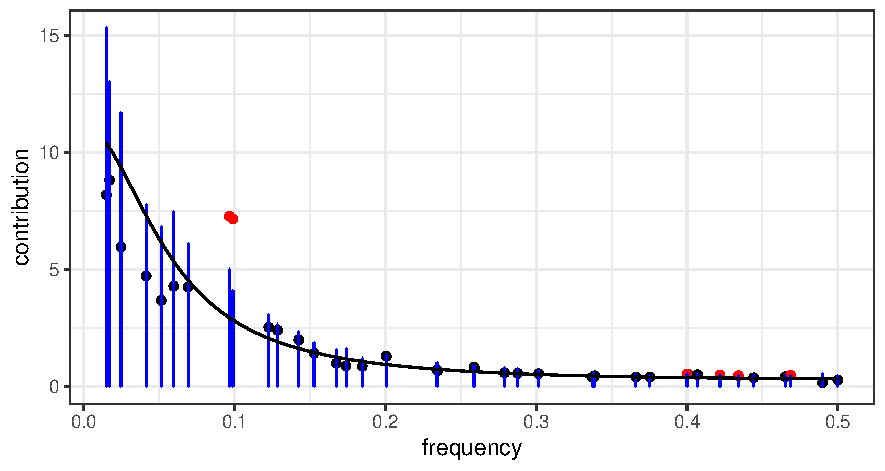
\includegraphics[width=0.7\textwidth]{img/mcssa_spec_phi7.pdf}
		\caption{Спектральная плотность при $\varphi=0.7$ (сигнал на частоте $\omega=0.1$)}
		\label{fig:mcssa_spec_phi7}
	\end{figure}
	\begin{figure}[h]
		\centering
		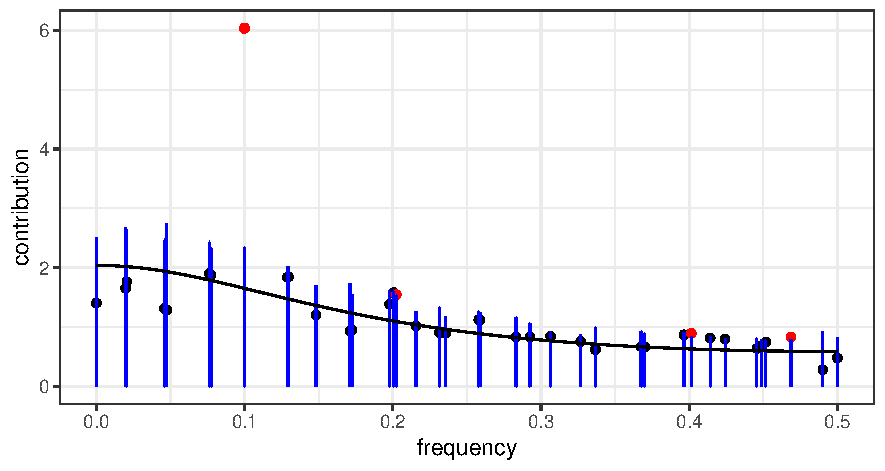
\includegraphics[width=0.7\textwidth]{img/mcssa_spec_phi3.pdf}
		\caption{Спектральная плотность при $\varphi=0.3$ (сигнал на частоте $\omega=0.1$)}
		\label{fig:mcssa_spec_phi3}
	\end{figure}
	\begin{figure}[H]
		\centering
		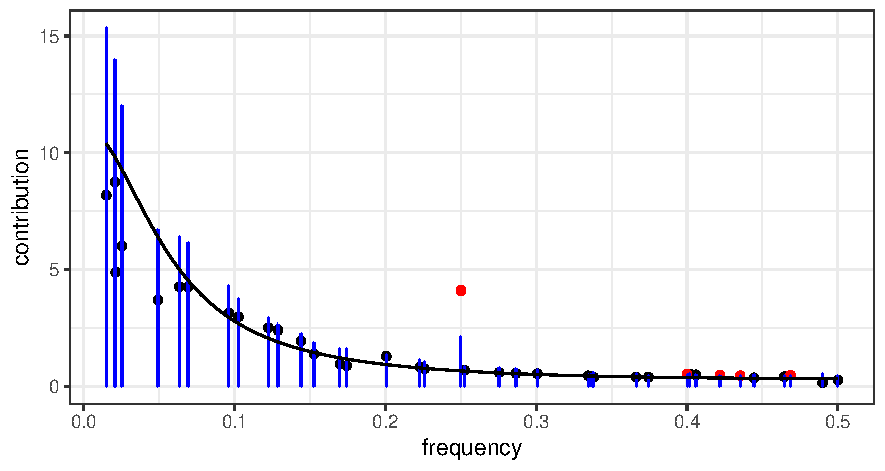
\includegraphics[width=0.7\textwidth]{img/mcssa_spec_phi7_omega025.pdf}
		\caption{Спектральная плотность при $\varphi=0.7$ (сигнал на частоте $\omega=0.25$)}
		\label{fig:mcssa_spec_phi7_omega025}
	\end{figure}
	При увеличении частоты $\omega$ сигнала значение спектральной плотности в этой точке уменьшается, что приводит к увеличению мощности критерия, это можно увидеть, сравнив рис.~\ref{fig:mcssa_spec_phi7} и~\ref{fig:mcssa_spec_phi7_omega025}.
\end{proof}

\subsection{Численное сравнение MC-SSA с другими критериями}\label{sect:mc-ssa_comparison}
Рассмотрим другие критерии проверки гипотезы о том, что временной ряд состоит из красного шума против альтернативы с наличием сигнала. Пусть дан временной ряд $\tX=\tS+\bfxi$, где $\tS$~--- сигнал, $\bfxi$~--- красный шум с параметрами $\varphi$ и $\delta$. Большинство критериев проверяет гипотезу о том, что временной ряд --- реализация белого шума. Поэтому будем действовать следующих образом:
\begin{enumerate}
	\item Провести отбеливание: вычислить $\tY=\Sigma^{-1/2}\tX$, где $\Sigma$~--- теоретическая автокорреляционная матрица красного шума с элементами $\varphi^{|i-j|}$, которая при верной $H_0$ совпадает с автокорреляционной матрицей ряда $\tX$.
	\item Проверить гипотезу о том, что $\tY$ является реализацией белого шума, с применением коррекции при необходимости.
\end{enumerate}
В качестве тестов на белый шум был взят Q-тест Бокса-Пирса~\cite{Box1970} и тест с использованием вейвлетов~\cite{Nason2014} (будем далее называть их box и wavelet). Отметим, что второй тест применим только к рядам длины $N=2^k$, где $k\in\mathbb{N}$. В связи с этим положим $N=128$, параметры шума возьмем $\varphi=0.7$, $\delta=1$. За альтернативу возьмем $\tS=\{A\cos(2\pi n\omega)\}_{n=1}^N$ и сравним мощность методов с отбеливанием и MC-SSA при помощи ROC-кривых для разных $\omega$. Для MC-SSA будем рассматривать теплицево разложение~\eqref{eq:sum_decomposition} траекторной матрицы. В силу предположения~\ref{statement1} для б\'{о}льших частот будем брать меньшую амплитуду сигнала с целью избежать слишком мощных критериев.

\begin{figure}[h!]
	\centering
	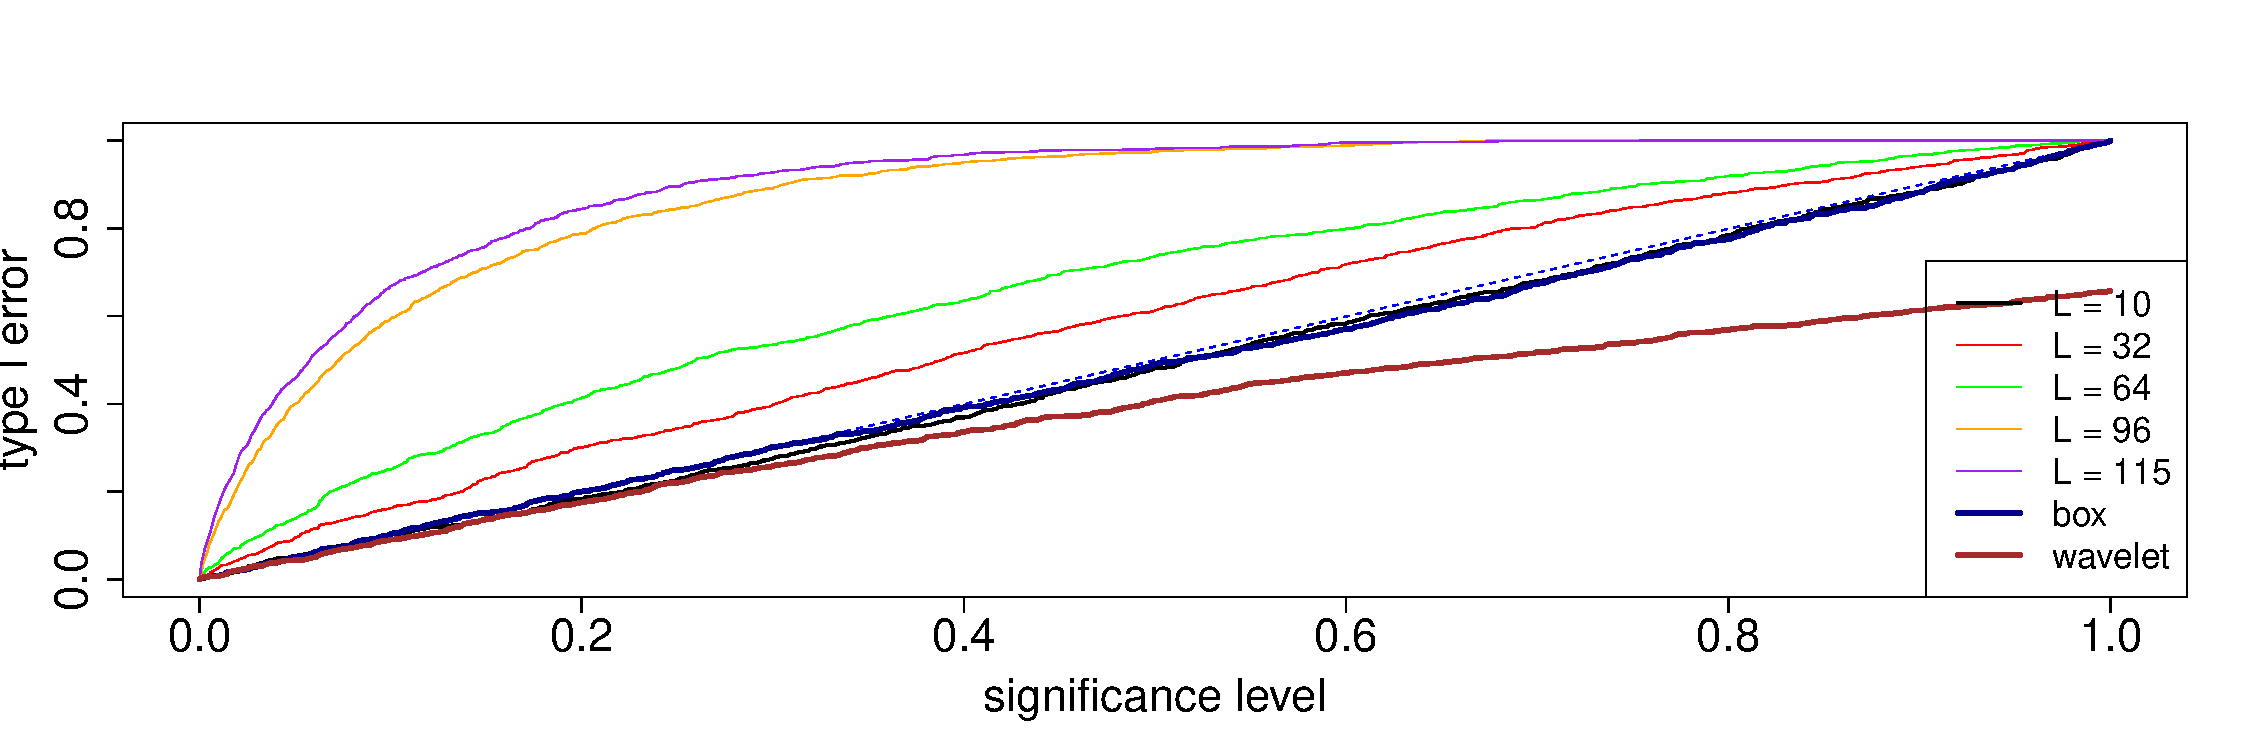
\includegraphics[width=0.7\textwidth]{img/alphaI_testAR.pdf}
	\caption{Сравнение ошибки I рода с другими методами}
	\label{alphaI_testAR}
\end{figure}

\begin{figure}[h!]
	\begin{subfigure}[t]{\textwidth}
		\centering
		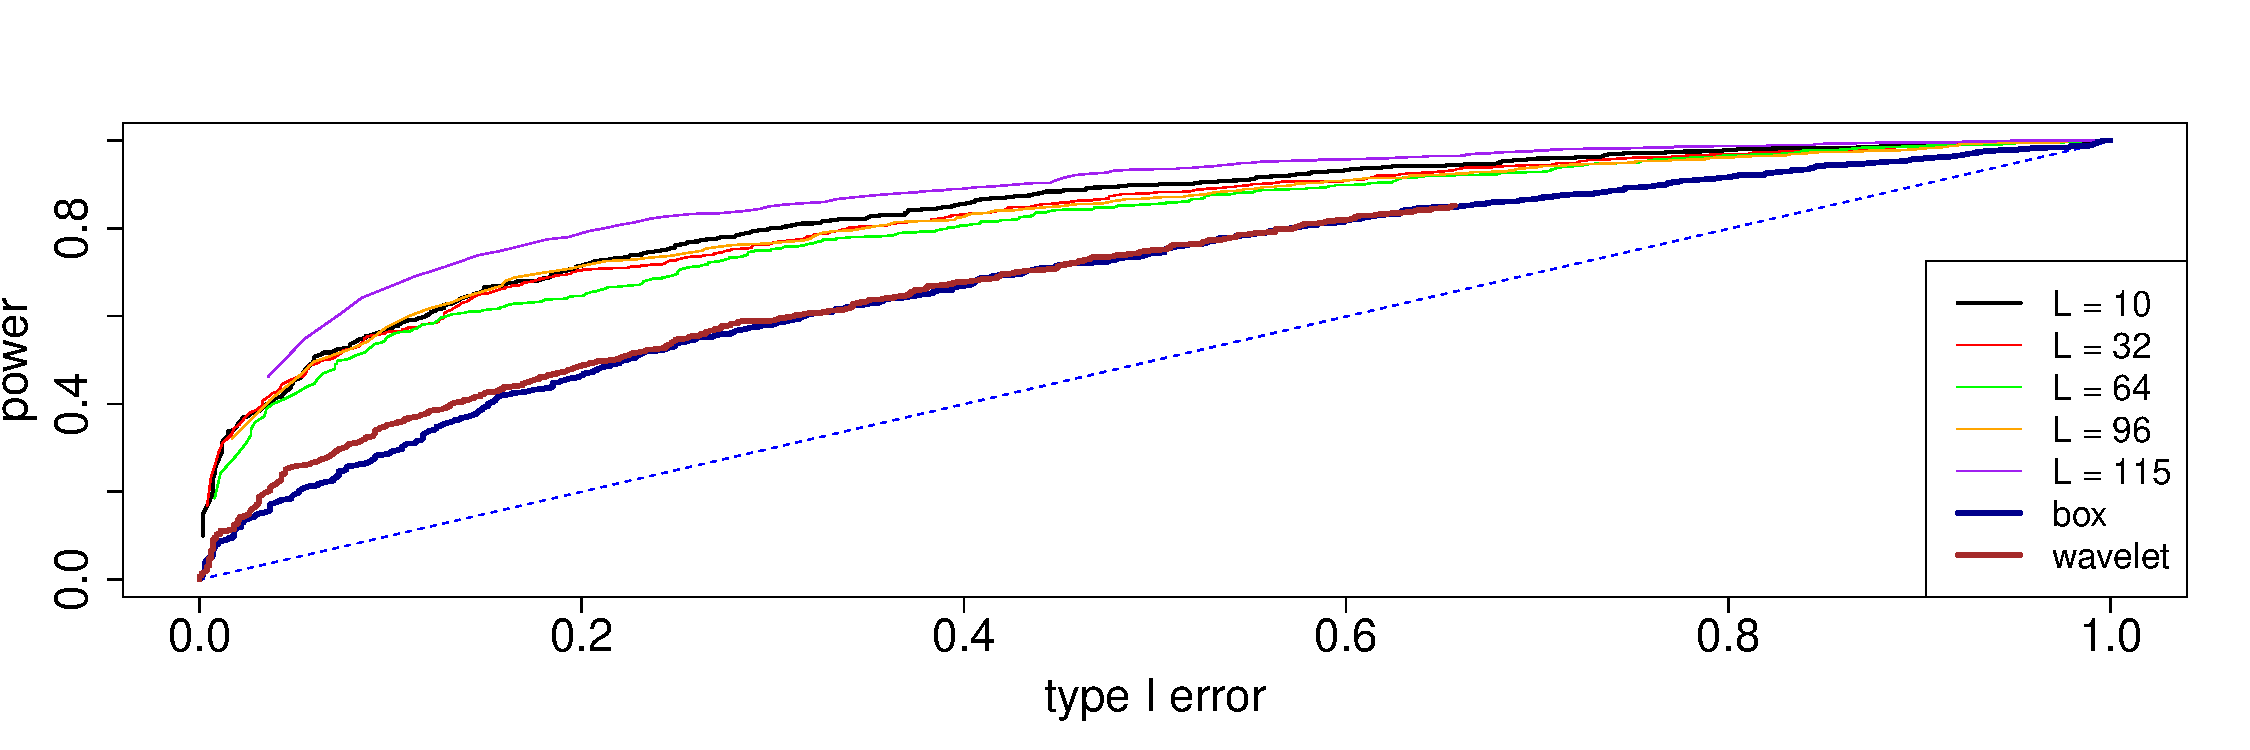
\includegraphics[width=0.7\textwidth]{img/roc_testAR_omega0025.pdf}
		\caption{ROC-кривая ($A=1.5$, $\omega=0.025$)}
		\label{roc_testAR_omega0025}
	\end{subfigure}
	\begin{subfigure}[t]{\textwidth}
		\centering
		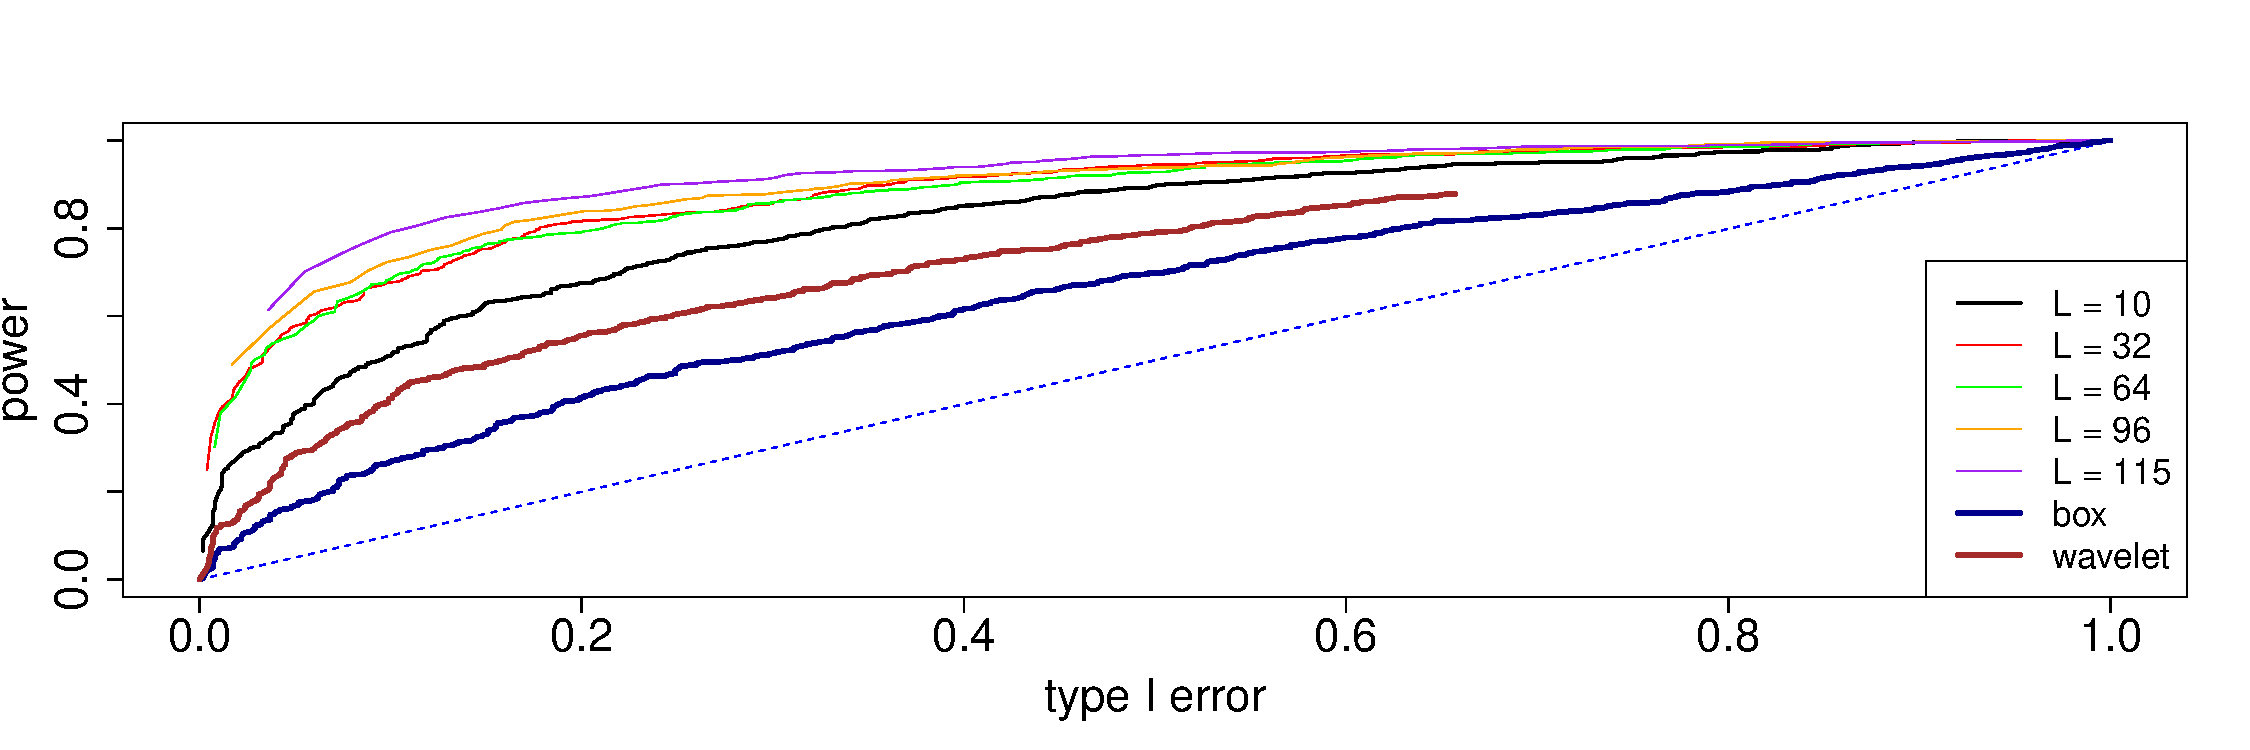
\includegraphics[width=0.7\textwidth]{img/roc_testAR_omega0125.pdf}
		\caption{ROC-кривая ($A=0.8$, $\omega=0.125$)}
		\label{roc_testAR_omega0125}
	\end{subfigure}
	\begin{subfigure}[t]{\textwidth}
		\centering
		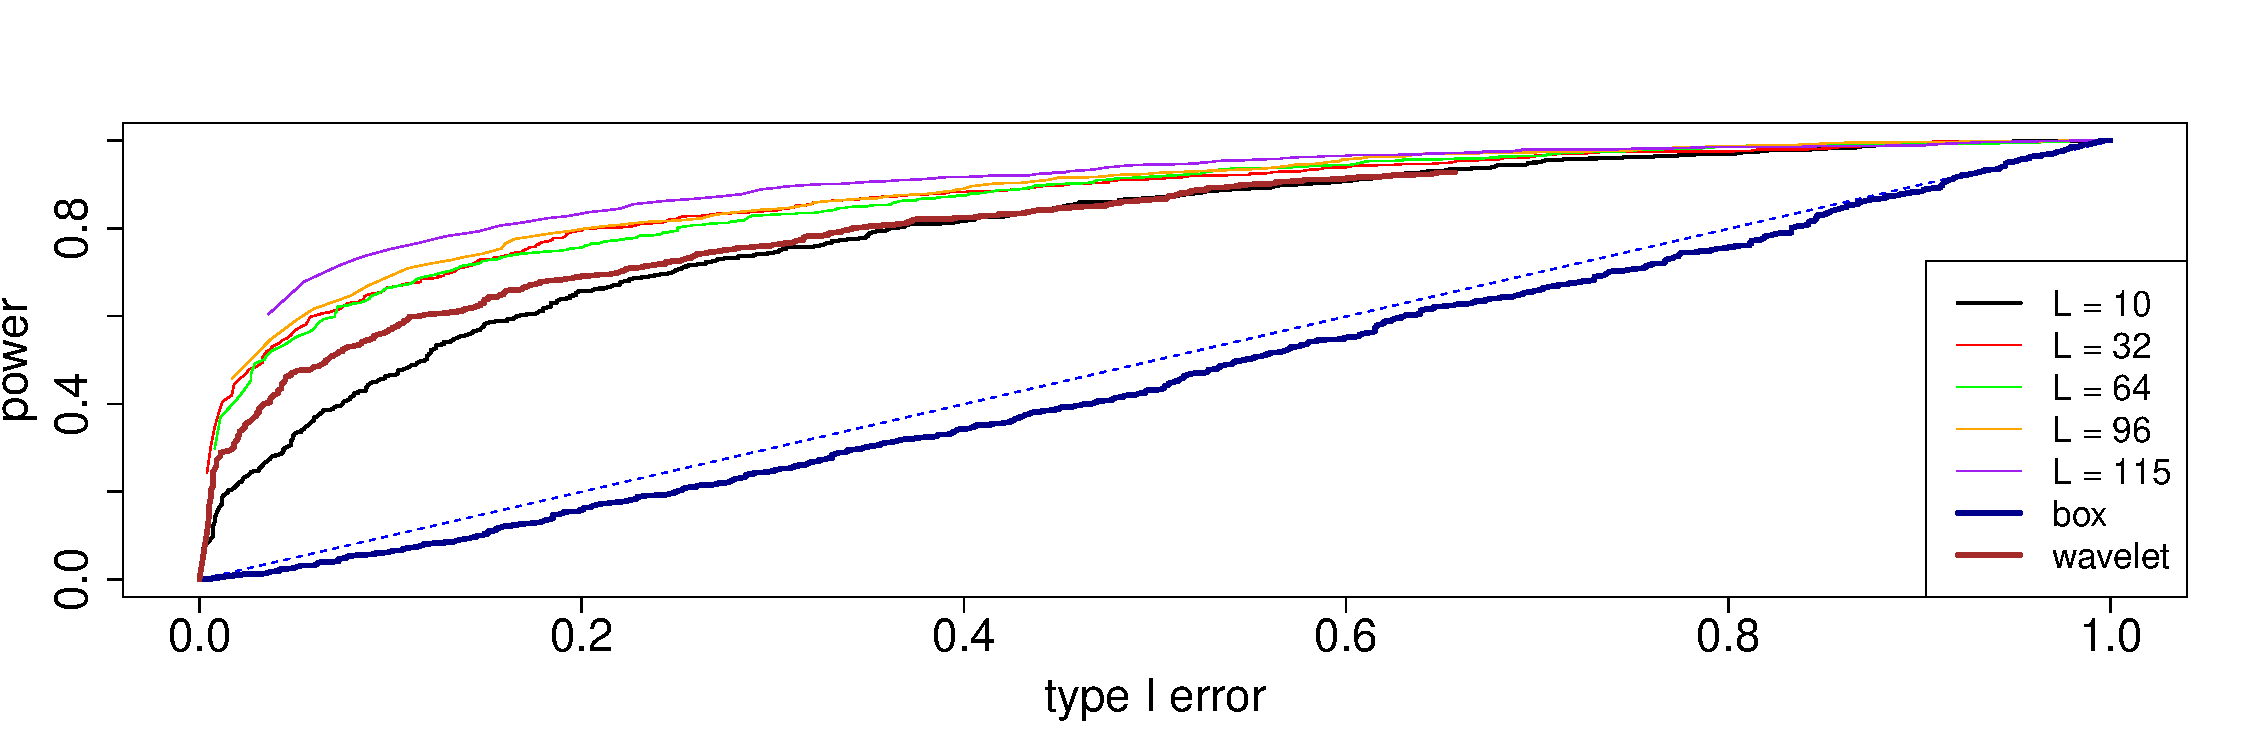
\includegraphics[width=0.7\textwidth]{img/roc_testAR_omega0225.pdf}
		\caption{ROC-кривая ($A=0.5$, $\omega=0.225$)}
		\label{roc_testAR_omega0225}
	\end{subfigure}
	\caption{Сравнение ROC-кривых с другими методами}
\end{figure}

\begin{table}[h!]
	\centering
	\caption{Результаты численного сравнения MC-SSA с другими критериями ($\alpha^*=0.1$)}
	\label{tab:comparison}
	\begin{tabular}{|cc>{\centering\arraybackslash}m{0.7in}>{\centering\arraybackslash}m{0.7in}>{\centering\arraybackslash}m{0.7in}|}\hline
		Метод & $\alpha_I(\alpha^*)$ & $\beta(\widetilde\alpha^*)$ $A=1.5$ $\omega=0.025$ & $\beta(\widetilde\alpha^*)$ $A=0.8$ $\omega=0.125$ & $\beta(\widetilde\alpha^*)$ $A=0.5$ $\omega=0.225$\\
		\hline
		MC-SSA ($L=10$) & 0.101 & 0.57 & 0.51 & 0.465\\
		\hline
		MC-SSA ($L=32$) & 0.163 & 0.566 & 0.678 & 0.668\\
	    \hline
	    MC-SSA ($L=64$) & 0.25 & 0.556 & 0.684 & 0.665\\
	    \hline
	    MC-SSA ($L=96$) & 0.593 & 0.599 & 0.734 & 0.709\\
	    \hline
	    MC-SSA ($L=115$) & 0.668 & 0.668 & 0.791 & 0.753\\
	    \hline
	    box & 0.103 & 0.289 & 0.269 & 0.064\\
	    \hline
	    wavelet & 0.091 & 0.354 & 0.414 & 0.57\\
	    \hline
	\end{tabular}
\end{table}

На рис.~\ref{roc_testAR_omega0025},~\ref{roc_testAR_omega0125},~\ref{roc_testAR_omega0225} изображены ROC-кривые методов при разных $\omega$. Отметим, что для wavelet построить ROC-кривые для больших ошибок I рода не удалось, поскольку на рис.~\ref{alphaI_testAR} видно, что $\alpha_I(\alpha) < 1$ $\forall \alpha$. Видно, при разработки критерия wavelet авторы делали его почти точным при $\alpha < 0.2$ и не заботились о том, что будет при б\'{о}льших значениях.

Для всех рассмотренных $\omega$ MC-SSA при всех длинах окна мощнее, чем box и wavelet, кроме случая с высокой частотой ($\omega=0.225$), где wavelet оказался немного мощнее MC-SSA с $L=10$. Отметим также, что на рис.~\ref{roc_testAR_omega0225} ROC-кривая метода box лежит ниже прямой $y=x$, поэтому этот тест не имеет смысл применять для выявления высоких частот. Для удобства сравнения в таблице~\ref{tab:comparison} для каждого критерия указана ошибка первого рода и мощность поправленного критерия для каждой рассмотренной альтернативы при уровне значимости $\alpha^*=0.1$.

\section{Monte Carlo MSSA}\label{sect:mc-mssa}
\subsection{Отличия от одномерного случая}
MC-SSA легко обобщается на многомерный случай: нужно просто заменить SSA на MSSA и генерировать красный шум с тем же количеством каналов, что и у исходного ряда~\cite{Groth2015}.

Стоит отметить, что, в отличие от одномерного случая, левые и правые векторы матрицы отличаются по построению $\bfX$~\eqref{eq:embedding_mssa}, поэтому в MC-MSSA в качестве векторов для проекции рассмотрены и левые, и правые векторы. Если $W_1,\ldots,W_H$~--- левые векторы матрицы $\bfX$, метод совпадает с алгоритмом~\ref{alg:multiple_mc-ssa}. Если рассматривать в качестве векторов для проекции правые векторы, то в формулах~\eqref{eq:mc-ssa_statisctics} и~\eqref{eq:mc-ssa_h0} нужно заменить $\bfX$ на $\bfX^\rmT$ и $\mathbf{\Xi}_i$ на $\mathbf{\Xi}_i^\rmT$ соответственно.

\subsection{Численное сравнение модификаций MC-MSSA}\label{sect:mc-mssa_numeric_comparison}
Поскольку рассматриваемый вариант критерия MC-(M)SSA является радикальным, нужно найти длину окна $L$, дающую максимально мощный критерий, но по замечанию~\ref{remark:liberal} он не должен быть слишком радикальным, чтобы можно было применить поправку, не увеличивая трудоемкость метода.

Введем понятие условно равномощных критериев. Поскольку оценка мощности критерия $\hat \beta$ является долей отвергнутых нулевых гипотез при верной альтернативе, соответствующий доверительный интервал для настоящего значения $\beta$ выглядит следующим образом:
\[
	\hat \beta \pm z_\alpha \sqrt{\frac{\hat \beta(1 - \hat \beta)}M},
\]
где $z_\alpha$~--- $(1-\alpha/2)$-квантиль $N(0, 1)$ и $M$~--- количество моделирований. В худшем случае ($\beta=0.5$) $95\%$-ный доверительный интервал при $M=1000$ примерно равен $\hat\beta \pm 0.03$. Поэтому будем условно считать критерии равномощными, если их мощности будут отличатся не более чем на $0.03$.

Как было показано в~\cite[Приложение  Б.2.4]{Larin2022}, метод MC-SSA с проекцией на левые (правые) векторы SVD разложения матрицы $\bfX$~\eqref{eq:svd} дает очень радикальный критерий для больших (малых) значений длины окна $L$, что делает невозможным построение поправки.

Однако, в одномерном случае было установлено~\cite{Larin2022}, что если вместо SVD разложения матрицы $\bfX$ использовать теплицево, то радикальность критерия уменьшается, и уже можно применить поправку. Установим, что будет в многомерном случае, если использовать модификации, описанные в разделе~\ref{sect:decomposition}.

Пусть количество каналов $D=2$, длина каждого канала равна $N=100$. Рассмотрим модель $\tX=\tS+\bfxi$, где $\bfxi$~--- красный шум с параметрами $\varphi$ и $\delta=1$, а $\tS$~--- сигнал с элементами
\[
s_n^{(1)}=s_n^{(2)}=A\cos(2\pi\omega n),\quad n=1,\ldots, N.
\]
Тогда нулевая гипотеза $H_0:A=0$ и альтернатива $H_1:A\ne0$.

Будем смотреть на графики ошибок первого рода и ROC-кривые критериев для длин окна $L=10$, $20$, $50$, $80$, $90$. Будем воспринимать ROC-кривую как график мощности критерия, к которому был применен алгоритм~\ref{alg:correction}.

Рассмотрим несколько примеров. В данном разделе графики ошибок I рода и ROC-кривые представлены только для первого примера, для остальных графики можно найти в разделе~\ref{appendix:mc-mssa_graphs}. Таблицы с результатами для каждого примера можно найти в разделе~\ref{appendix:mc-mssa_tables}.

\begin{example}\label{mc-mssa_example1}
	Пусть $\varphi=0.7$ и параметры сигнала $A=1$, $\omega=0.075$.
\begin{figure}[H]
	\captionsetup[subfigure]{justification=Centering}
	\begin{subfigure}[t]{0.5\textwidth}
		\centering
		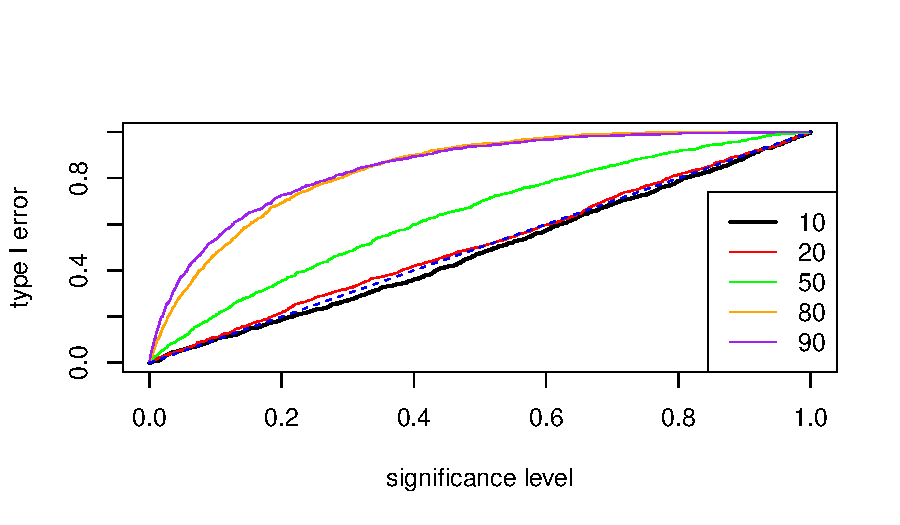
\includegraphics[width=0.9\textwidth]{img/type1error_sum_ev.pdf}
		\caption{Ошибка первого рода (Sum)}
		\label{fig:sum_ev_a}
	\end{subfigure}\hspace{\fill}
	\begin{subfigure}[t]{0.5\textwidth}
		\centering
		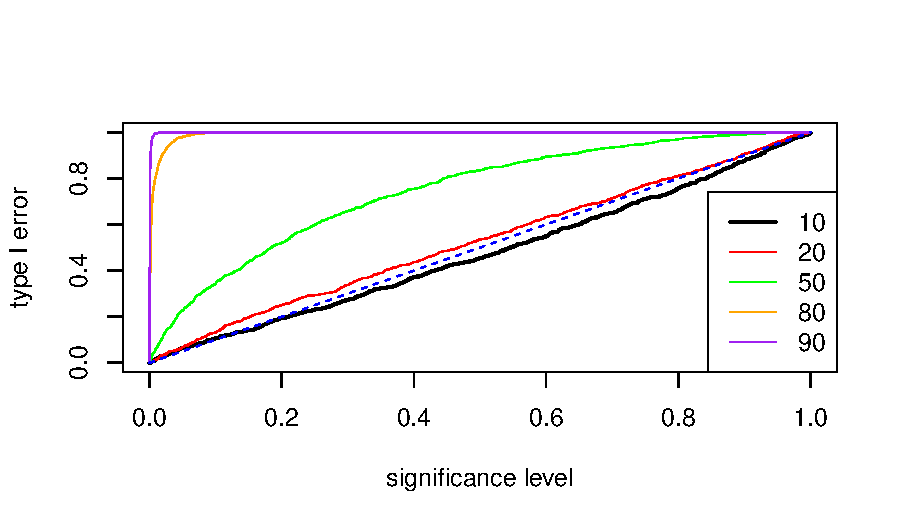
\includegraphics[width=0.9\textwidth]{img/type1error_mssa_ev.pdf}
		\caption{Ошибка первого рода (SVD)}
	\end{subfigure}
	\bigskip
	\begin{subfigure}[t]{0.5\textwidth}
		\centering
		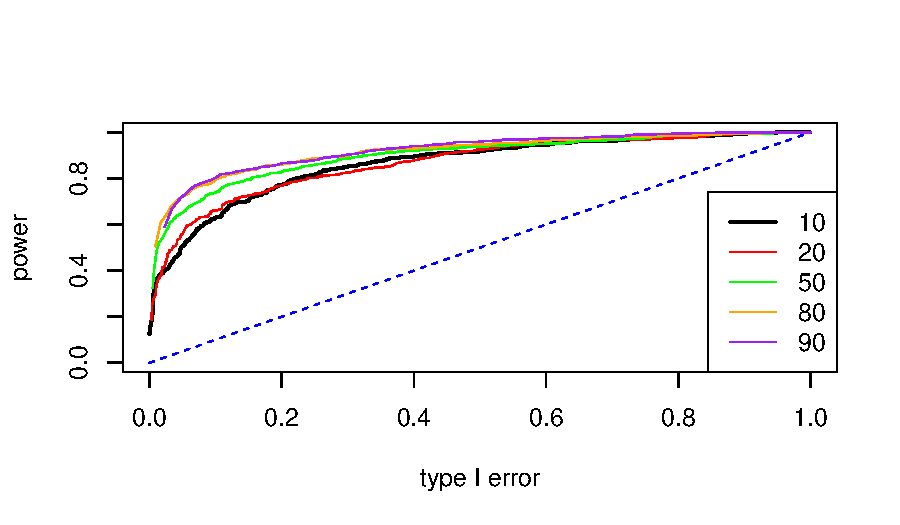
\includegraphics[width=0.9\textwidth]{img/roc_sum_ev_omega0075.pdf}
		\caption{ROC-кривая (Sum)}
		\label{fig:sum_ev_r}
	\end{subfigure}\hspace{\fill}
	\begin{subfigure}[t]{0.5\textwidth}
		\centering
		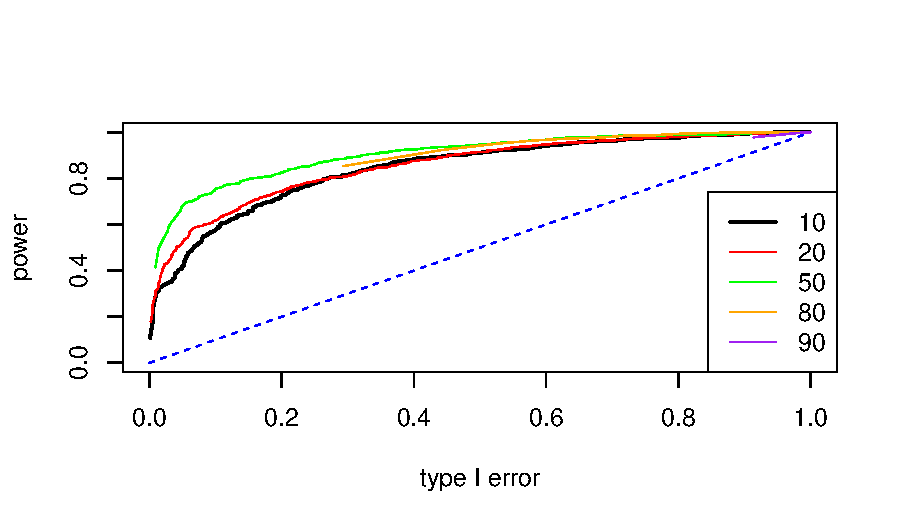
\includegraphics[width=0.9\textwidth]{img/roc_mssa_ev.pdf}
		\caption{ROC-кривая (SVD)}
	\end{subfigure}
	\caption{Сравнение методов с проекцией на левые векторы ($\varphi=0.7$, $A=1$, $\omega=0.075$)}
	\label{fig:sum_ev}
\end{figure}
\begin{figure}[H]
	\captionsetup[subfigure]{justification=Centering}
	\begin{subfigure}[t]{0.5\textwidth}
		\centering
		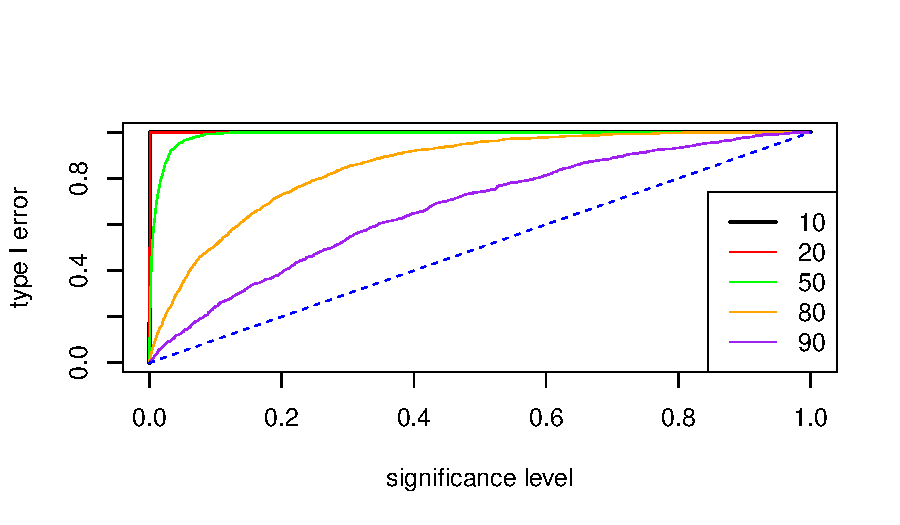
\includegraphics[width=0.9\textwidth]{img/type1error_sum_fa.pdf}
		\caption{Ошибка первого рода (Sum)}
		\label{fig:sum_fa_a}
	\end{subfigure}\hspace{\fill}
	\begin{subfigure}[t]{0.5\textwidth}
		\centering
		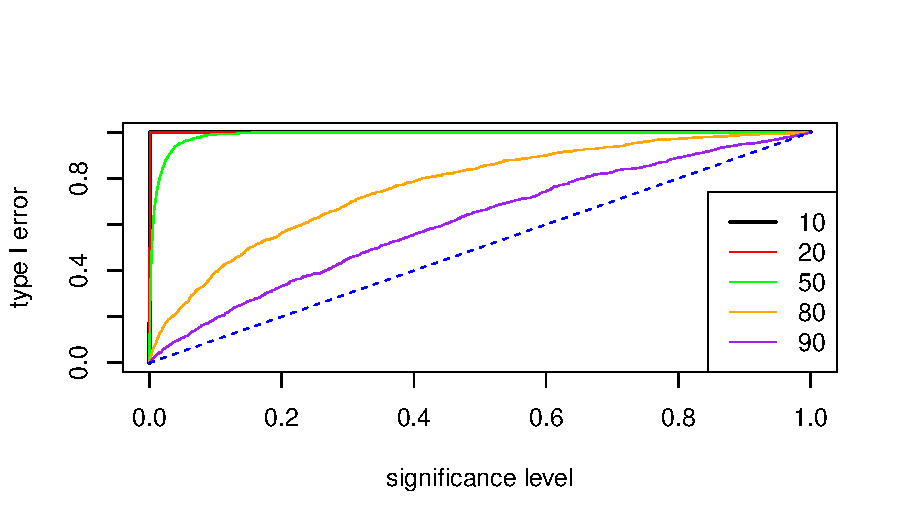
\includegraphics[width=0.9\textwidth]{img/type1error_mssa_fa.pdf}
		\caption{Ошибка первого рода (SVD)}
	\end{subfigure}
	\bigskip
	\begin{subfigure}[t]{0.5\textwidth}
		\centering
		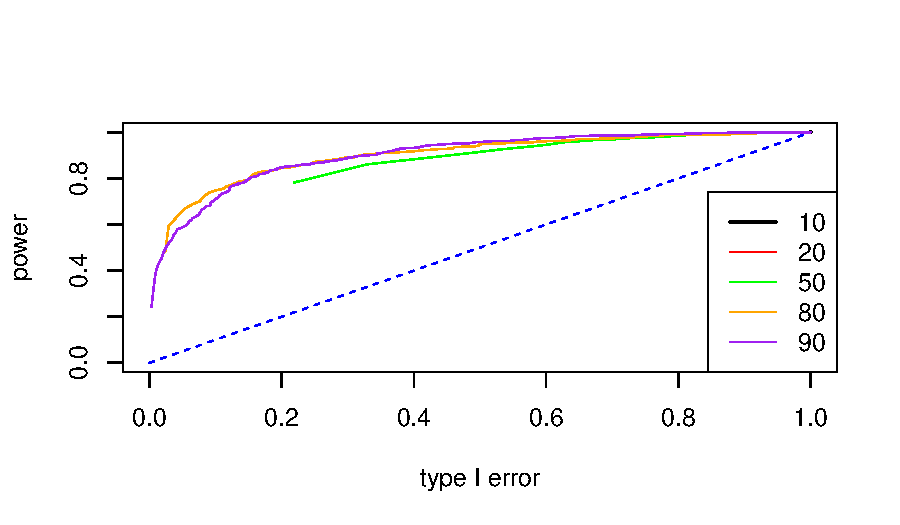
\includegraphics[width=0.9\textwidth]{img/roc_sum_fa_omega0075.pdf}
		\caption{ROC-кривая (Sum)}
		\label{fig:sum_fa_r}
	\end{subfigure}\hspace{\fill}
	\begin{subfigure}[t]{0.5\textwidth}
		\centering
		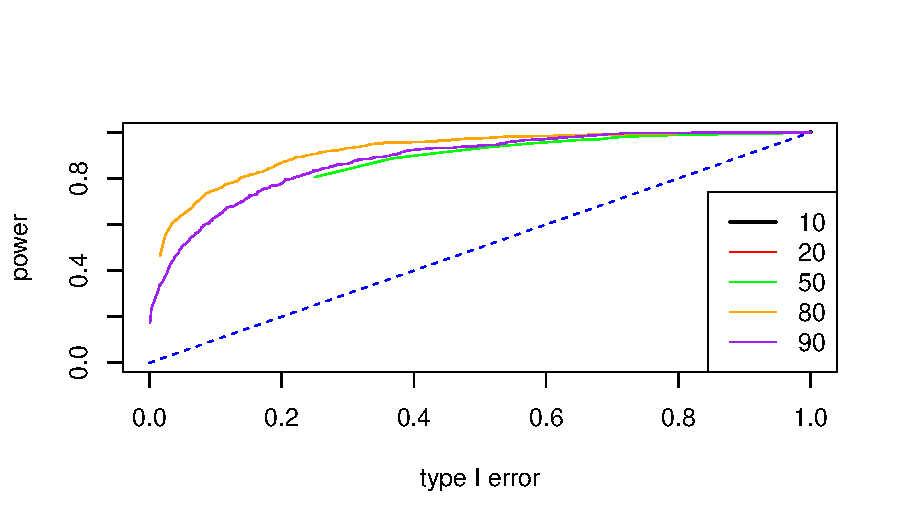
\includegraphics[width=0.9\textwidth]{img/roc_mssa_fa.pdf}
		\caption{ROC-кривая (SVD)}
	\end{subfigure}
	\caption{Сравнение методов с проекцией на правые векторы ($\varphi=0.7$, $A=1$, $\omega=0.075$)}
	\label{fig:sum_fa}
\end{figure}

\begin{figure}[H]
	\captionsetup[subfigure]{justification=Centering}
	\begin{subfigure}[t]{0.5\textwidth}
		\centering
		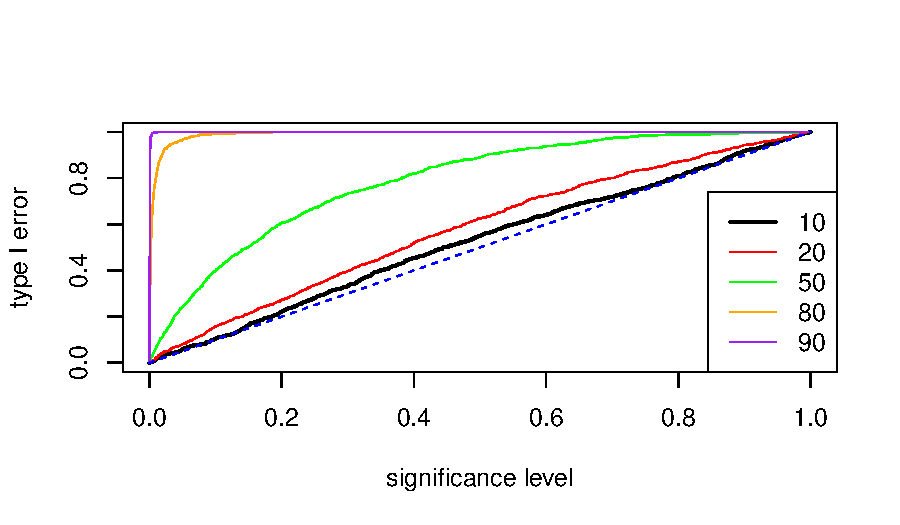
\includegraphics[width=0.9\textwidth]{img/type1error_block_ev.pdf}
		\caption{Ошибка первого рода (Block)}
		\label{fig:block_ev_a}
	\end{subfigure}\hspace{\fill}
	\begin{subfigure}[t]{0.5\textwidth}
		\centering
		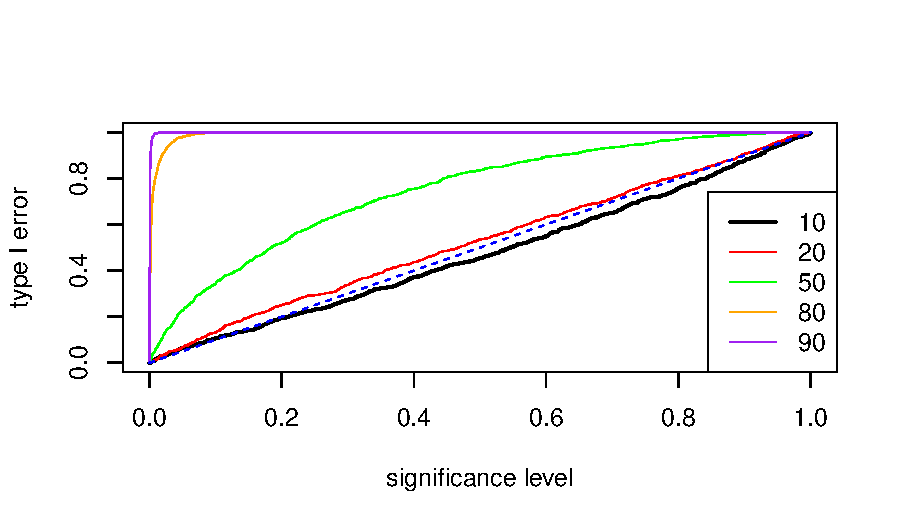
\includegraphics[width=0.9\textwidth]{img/type1error_mssa_ev.pdf}
		\caption{Ошибка первого рода (SVD)}
	\end{subfigure}
	\bigskip
	\begin{subfigure}[t]{0.5\textwidth}
		\centering
		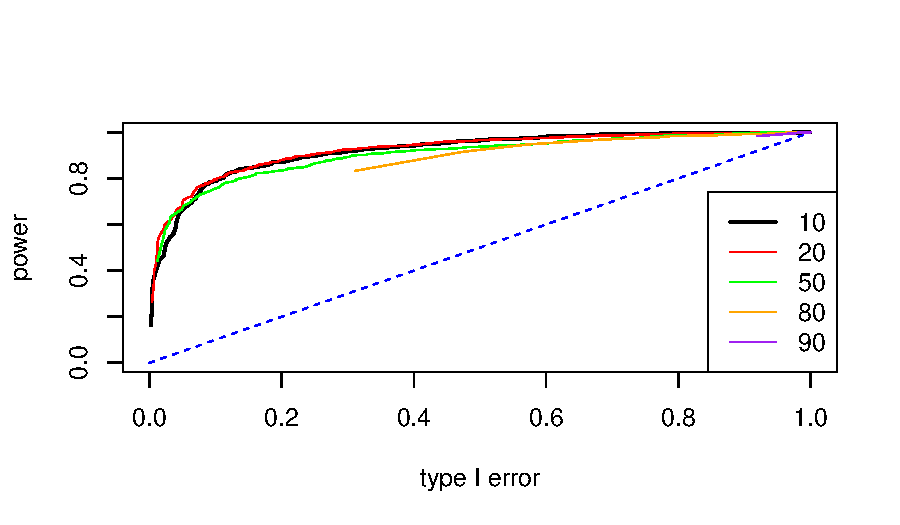
\includegraphics[width=0.9\textwidth]{img/roc_block_ev_omega0075.pdf}
		\caption{ROC-кривая (Block)}
		\label{fig:block_ev_r}
	\end{subfigure}\hspace{\fill}
	\begin{subfigure}[t]{0.5\textwidth}
		\centering
		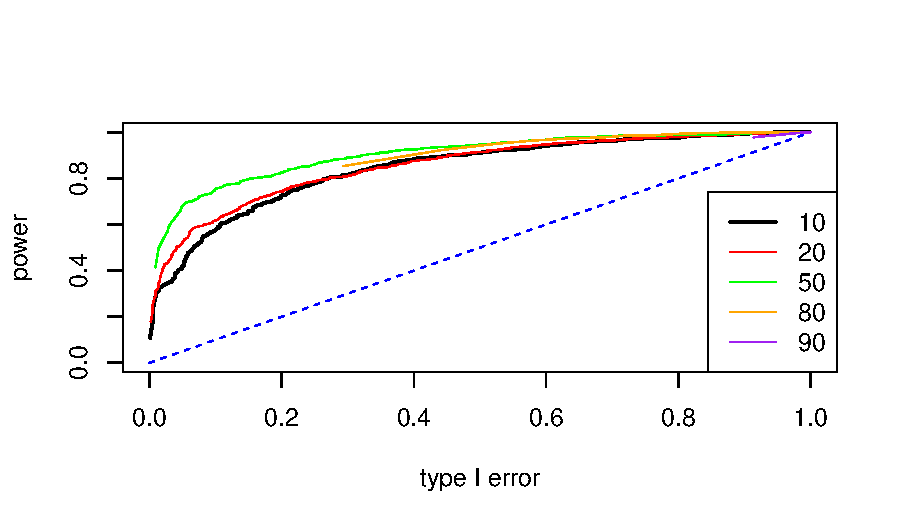
\includegraphics[width=0.9\textwidth]{img/roc_mssa_ev.pdf}
		\caption{ROC-кривая (SVD)}
	\end{subfigure}
	\caption{Сравнение методов с проекцией на левые векторы ($\varphi=0.7$, $A=1$, $\omega=0.075$)}
	\label{fig:block_ev}
\end{figure}
\begin{figure}[H]
	\captionsetup[subfigure]{justification=Centering}
	\begin{subfigure}[t]{0.5\textwidth}
		\centering
		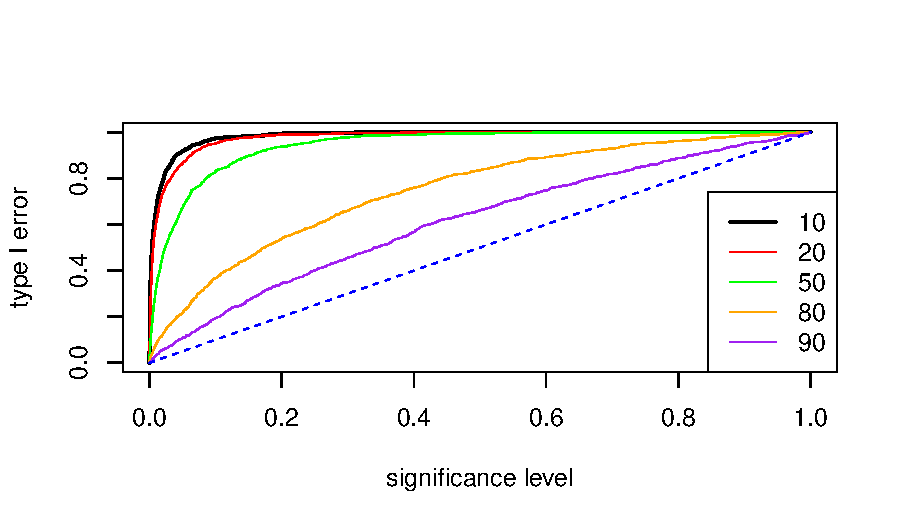
\includegraphics[width=0.9\textwidth]{img/type1error_block_fa.pdf}
		\caption{Ошибка первого рода (Block)}
		\label{fig:block_fa_a}
	\end{subfigure}\hspace{\fill}
	\begin{subfigure}[t]{0.5\textwidth}
		\centering
		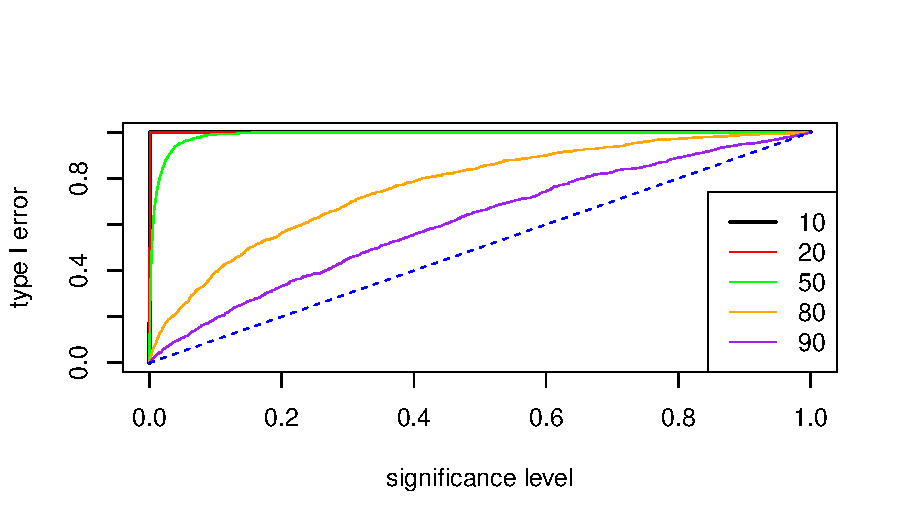
\includegraphics[width=0.9\textwidth]{img/type1error_mssa_fa.pdf}
		\caption{Ошибка первого рода (SVD)}
	\end{subfigure}
	\bigskip
	\begin{subfigure}[t]{0.5\textwidth}
		\centering
		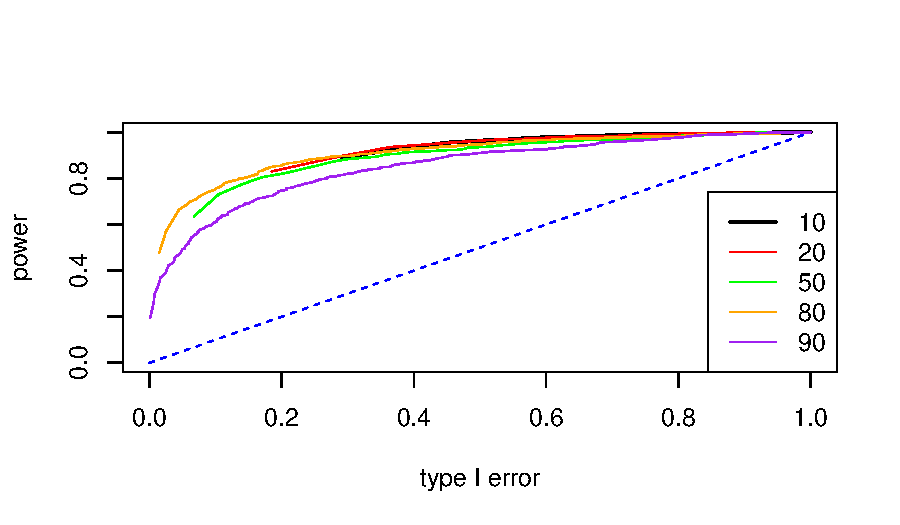
\includegraphics[width=0.9\textwidth]{img/roc_block_fa_omega0075.pdf}
		\caption{ROC-кривая (Block)}
		\label{fig:block_fa_r}
	\end{subfigure}\hspace{\fill}
	\begin{subfigure}[t]{0.5\textwidth}
		\centering
		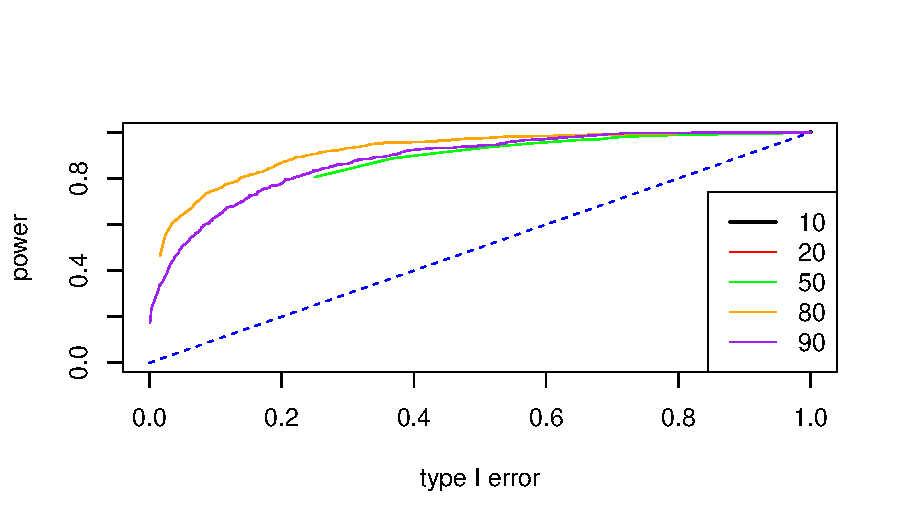
\includegraphics[width=0.9\textwidth]{img/roc_mssa_fa.pdf}
		\caption{ROC-кривая (SVD)}
	\end{subfigure}
	\caption{Сравнение методов с проекцией на правые векторы ($\varphi=0.7$, $A=1$, $\omega=0.075$)}
	\label{fig:block_fa}
\end{figure}

На рис.~\ref{fig:sum_ev} и~\ref{fig:sum_fa} векторы для проекции были взяты из разложения~\eqref{eq:sum_decomposition}. На рис.~\ref{fig:sum_ev_a} видно, что при $L>20$ метод радикальный, а наибольшая мощность достигается при $L=90$. На рис.~\ref{fig:sum_fa_a} отчетливо заметно, что метод радикальный для всех $L$. Наибольшая мощность наблюдается при $L=80$, но отметим, что из-за слишком большой ошибки первого рода построить ROC-кривую на промежутке $[0,0.22)$ для $L=50$ и на всем промежутке для $L=10$ и $L=20$ не получилось.

На рис.~\ref{fig:block_ev} и~\ref{fig:block_fa} векторы для проекции были взяты из разложения~\eqref{eq:block_decomposition}. Если рассматривать проекцию на левые векторы, то на рис.~\ref{fig:block_ev_a} видно, что метод радикальный, а наибольшая мощность достигается при $L=20$. Проекция на правые векторы также дает радикальный критерий, как видно на рис.~\ref{fig:block_fa_a}. Наибольшая мощность наблюдается при $L=80$, но из-за слишком большой ошибки первого рода ROC-кривую для $L=10$ и $L=20$, для которых метод, предположительно, имеет б\'oльшую мощность, удалось построить не на всем промежутке.
\end{example}

\begin{example}~\label{mc-mssa_example2}
	Пусть $\varphi=0.3$ и $\omega=0.075$. В виду предположения~\ref{statement1} уменьшим амплитуду сигнала для этого примера до $A=0.5$.
\end{example}

\begin{example}~\label{mc-mssa_example3}
	В условиях примера~\ref{mc-mssa_example1} увеличим частоту сигнала до $\omega=0.225$ и в силу предположения~\ref{statement1} уменьшим амплитуду сигнала до $A=0.4$.
\end{example}

\begin{table}[h]
	\caption{Мощность методов для оптимальных $L$ ($\alpha^*=0.1$)}
	\label{tab:res_mc-ssa_power}
	\centering
	\begin{tabular}{|c>{\centering\arraybackslash}m{1in}>{\centering\arraybackslash}m{1in}>{\centering\arraybackslash}m{1in}>{\centering\arraybackslash}m{1in}|}\hline
		Метод & левые/правые векторы & $\beta(\widetilde\alpha^*)$ (пример 1) & $\beta(\widetilde\alpha^*)$ (пример 2) & $\beta(\widetilde\alpha^*)$ (пример 3)\\
		\hline
		SVD & левые & 0.754 & \textbf{0.399} & 0.573 \\
		\hline
		SVD & правые & 0.754 & 0.382 & 0.442 \\
		\hline
		Block & левые & \textbf{0.796} & \textbf{0.398} & \textbf{0.597} \\
		\hline
		Block & правые & 0.717 & 0.389 & 0.473 \\
		\hline
		Sum & левые & \textbf{0.806} & \textbf{0.421} & \textbf{0.625} \\
		\hline
		Sum & правые & 0.748 & \textbf{0.412} & \textbf{0.613} \\
		\hline
	\end{tabular}
\end{table}

\begin{table}[h]
	\caption{Размеры матриц методов}
	\label{tab:res_mc-ssa_complexity}
	\centering
	\begin{tabular}{|c>{\centering\arraybackslash}m{1in}>{\centering\arraybackslash}m{1in}>{\centering\arraybackslash}m{1in}>{\centering\arraybackslash}m{1in}|}\hline
		Метод & левые/правые векторы & Размер матрицы (пример 1) & Размер матрицы (пример 2) & Размер матрицы (пример 3) \\
		\hline
		SVD & левые & 50 & 10 & 20 \\
		\hline
		SVD & правые & 80 & 80 & 80 \\
		\hline
		Block & левые & 102 & 162 & 162 \\
		\hline
		Block & правые & 42 & 22 & 42\\
		\hline
		Sum & левые & 80 & 20 & 80 \\
		\hline
		Sum & правые & 80 & 80 & 80 \\
		\hline
	\end{tabular}
\end{table}

В таблице~\ref{tab:res_mc-ssa_power} представлены мощности поправленных критериев при уровне значимости $\alpha^*=0.1$ для оптимальной длины окна для каждого рассмотренного примера, черным выделены наибольшая мощность и примерно равные ей (отличающиеся не более, чем на 0.03). В таблице~\ref{tab:res_mc-ssa_complexity} представлены размеры матриц методов, у которых находятся вектора для проекции для тех длин окна, мощность которых примерно равна мощности при оптимальном $L$, но критерии с такой длиной окна более эффективные (матрица меньшего размера). Из замечания~\ref{remark:complexity} следует, что трудоемкость метода MC-MSSA равна трудоемкости разложения матрицы выбранного метода, умноженной на $M$.

\subsubsection{Выводы}
Подведем итоги. Для рассмотренных примеров методы Block и Sum c проекцией на левые векторы показывают наибольшую мощность среди всех рассмотренных модификаций MC-MSSA, однако, учитывая таблицу~\ref{tab:res_mc-ssa_complexity} и замечания~\ref{remark:mssa_complexity},~\ref{remark:complexity}, метод Sum во всех трех случаях численно эффективнее метода Block в нахождении векторов для проекции. Также хочется отметить, что метод Sum с проекцией на левые векторы дает наименее радикальный критерий, что важно при построении поправки (см. замечание~\ref{remark:liberal}). Поэтому на данный момент, беря в учет рассмотренные примеры, рекомендуется использовать метод Sum с проекцией на левые векторы c $L=90$ для рядов длины $N=100$.

\chapter{Применение метода Monte Carlo SSA на практике}\label{chpt:mc_ssa_real}
В главе~\ref{chpt:mc-ssa} предполагалось, что параметры шума известны и нет мешающего сигнала (например, сезонности или тренда). Мешающий сигнал~--- это сигнал, который уже не нужно обнаруживать при проверки гипотезы о наличии сигнала.  В этой главе рассмотрим случаи, которые более близки к реальным задачам.

В разделе~\ref{sect:cps2024} исследована зависимость радикальности и мощности MC-SSA от длины окна на различных примерах. В разделе~\ref{sect:phi_est} рассмотрен один из способов оценки параметров красного шума и численное сравнение MC-SSA с известными и оцененными параметрами в разделе~\ref{sect:mc-ssa_est}. В разделе~\ref{sect:nuisance} приведены два алгоритма модификации MC-SSA с мешающим сигналом и проведено численное исследование методов для разных примеров мешающего сигнала. В разделе~\ref{sect:examples} рассмотрены примеры реальных временных рядов и их анализ с помощью SSA и MC-SSA.

В этой главе будем использовать MC-SSA с проекцией на векторы теплицева разложения~\eqref{eq:block_decomposition} матрицы $\bfX$.

\section{Зависимость радикальности и мощности от параметра $L$}~\label{sect:cps2024}
Поскольку рассматриваемый вариант критерия MC-SSA является радикальным, существует проблема выбора такой длины окна $L$, которая дает максимально мощный критерий, но при этом не слишком радикальный, чтобы можно было применить поправку из алгоритма~\ref{alg:correction}. Однако, в зависимости от длины ряда $N$ и параметров красного шума $\bfxi$ наблюдаются разные зависимости мощности от $L$.

Рассмотрим несколько примеров. Пусть дана модель
\[
    \tX=\tS+{\boldsymbol\xi},
\]
где $\tS=\{A\cos(2\pi\omega n)\}_{n=1}^N$, а ${\boldsymbol\xi}$~--- красный шум с параметрами $\varphi$ и $\delta=1$. Рассмотрим следующие нулевую гипотезу и альтернативу: $H_0:A=0$, $H_1:A\ne0$. В этом разделе будем предполагать, что параметры красного шума известны. В первых трех примерах рассмотрим частоту сигнала $\omega = 0.075$.

\begin{example}\label{example1}
	Пусть $\varphi=0.7$, $N=100$.
	\begin{figure}[h!]
		\captionsetup[subfigure]{justification=Centering}
		\begin{subfigure}[t]{\textwidth}
			\centering
			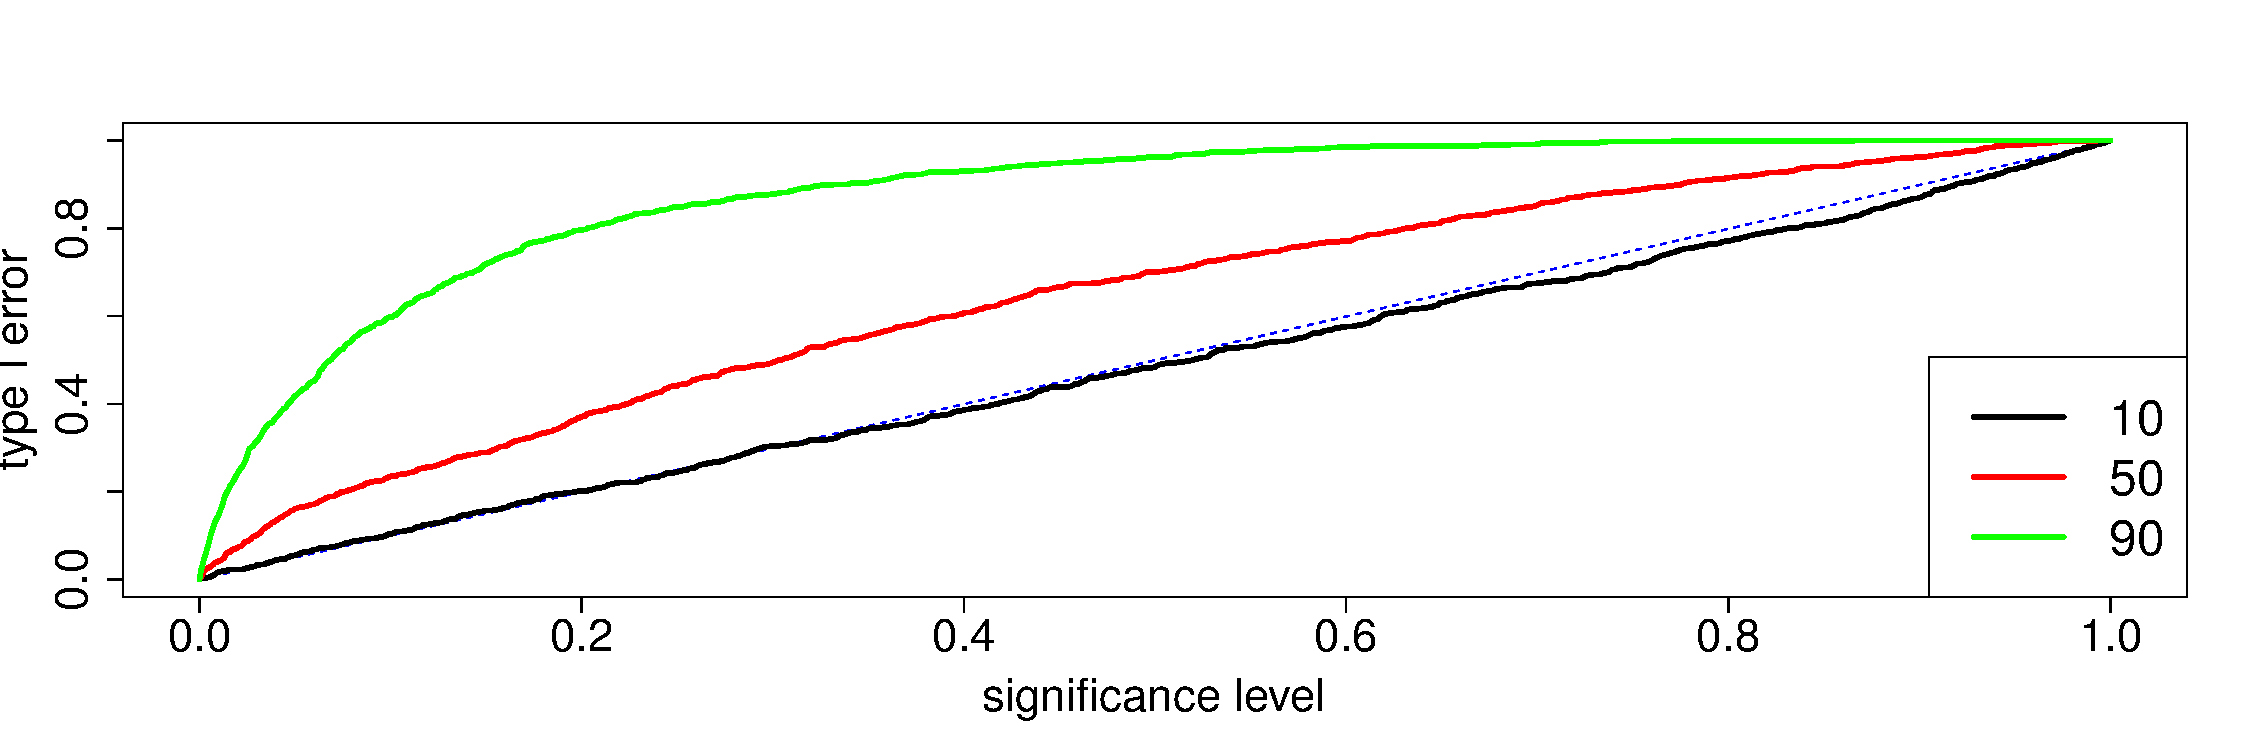
\includegraphics[width=0.7\textwidth]{img/alphaI_phi7_N100}
			\caption{Ошибка I рода}
			\label{alphaI_phi7_N100}
		\end{subfigure}
		\begin{subfigure}[t]{\textwidth}
			\centering
			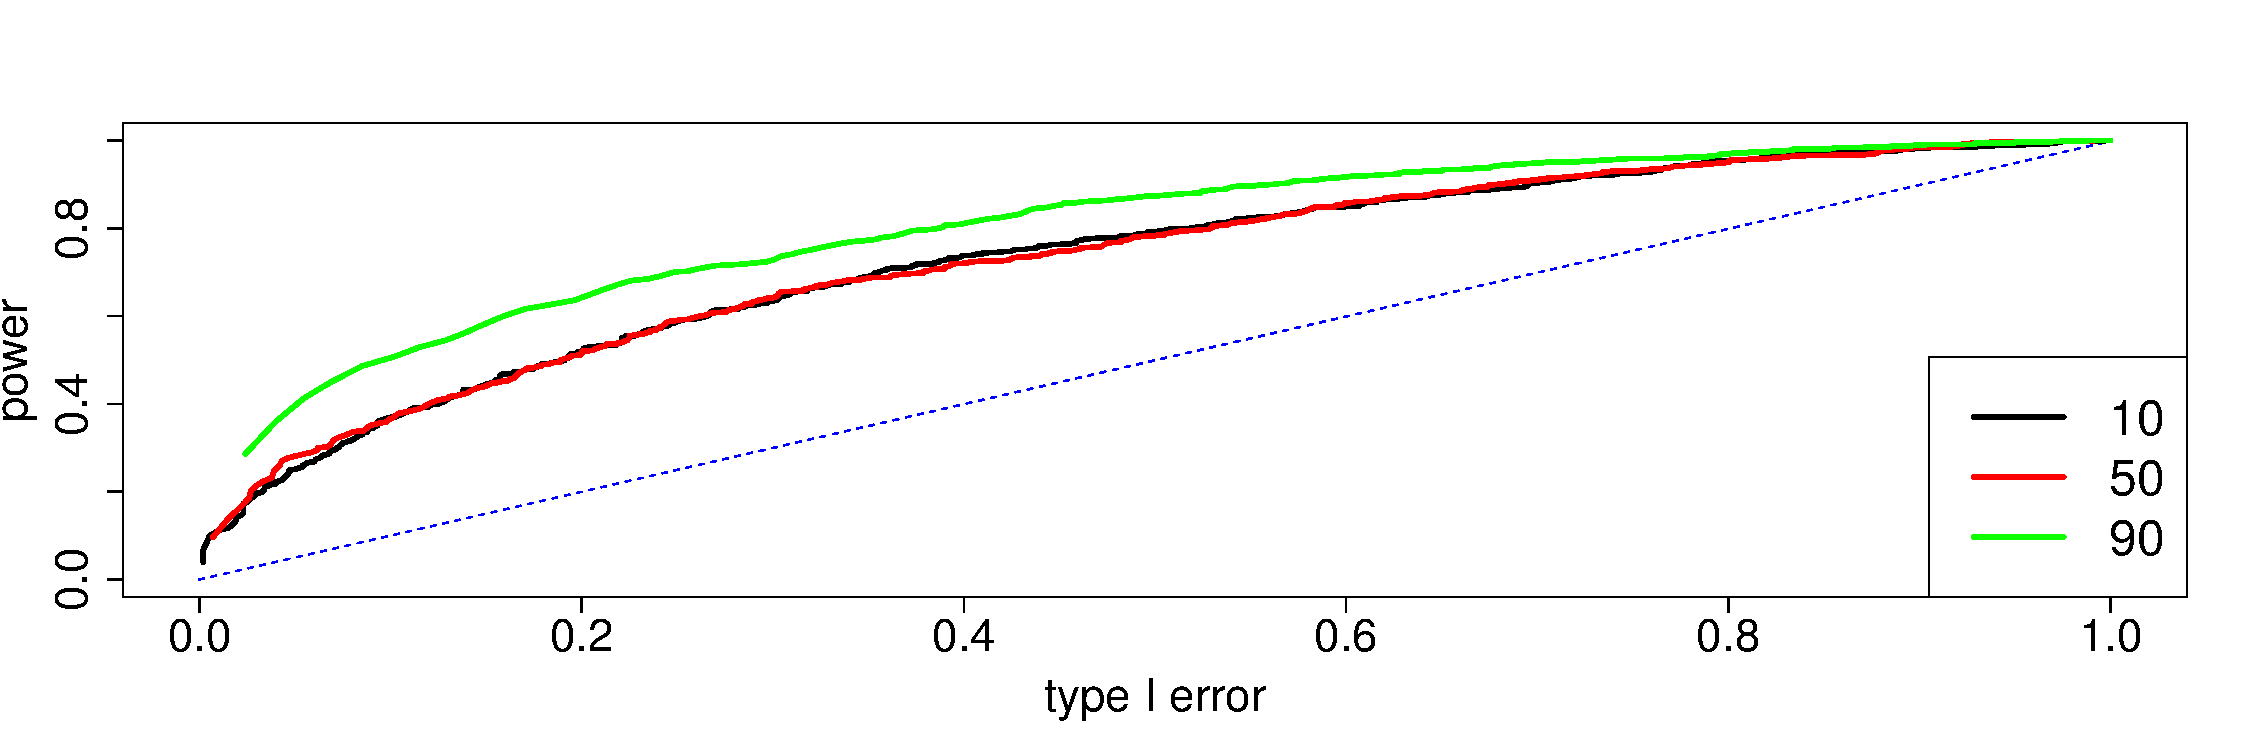
\includegraphics[width=0.7\textwidth]{img//roc_phi7_N100}
			\caption{ROC-кривая ($A=1$, $\omega=0.075$)}
			\label{roc_phi7_N100}
		\end{subfigure}
	\label{fig:example1}
	\caption{Пример~\ref{example1} ($\varphi=0.7$, $N=100$)}
	\end{figure}
	По графику ошибок первого рода на рис.~\ref{alphaI_phi7_N100} видно, что чем больше $L$, тем более радикальным становится критерий. На рис.~\ref{roc_phi7_N100} изображены ROC-кривые критериев, наибольшую мощность дает критерий с $L=90$. На этом примере видно, что самым мощным является самый радикальный критерий.
\end{example}

\begin{example}\label{example2}
	Пусть $\varphi=0.3$, $N=100$.
	\begin{figure}[h!]
		\captionsetup[subfigure]{justification=Centering}
		\begin{subfigure}[t]{\textwidth}
			\centering
			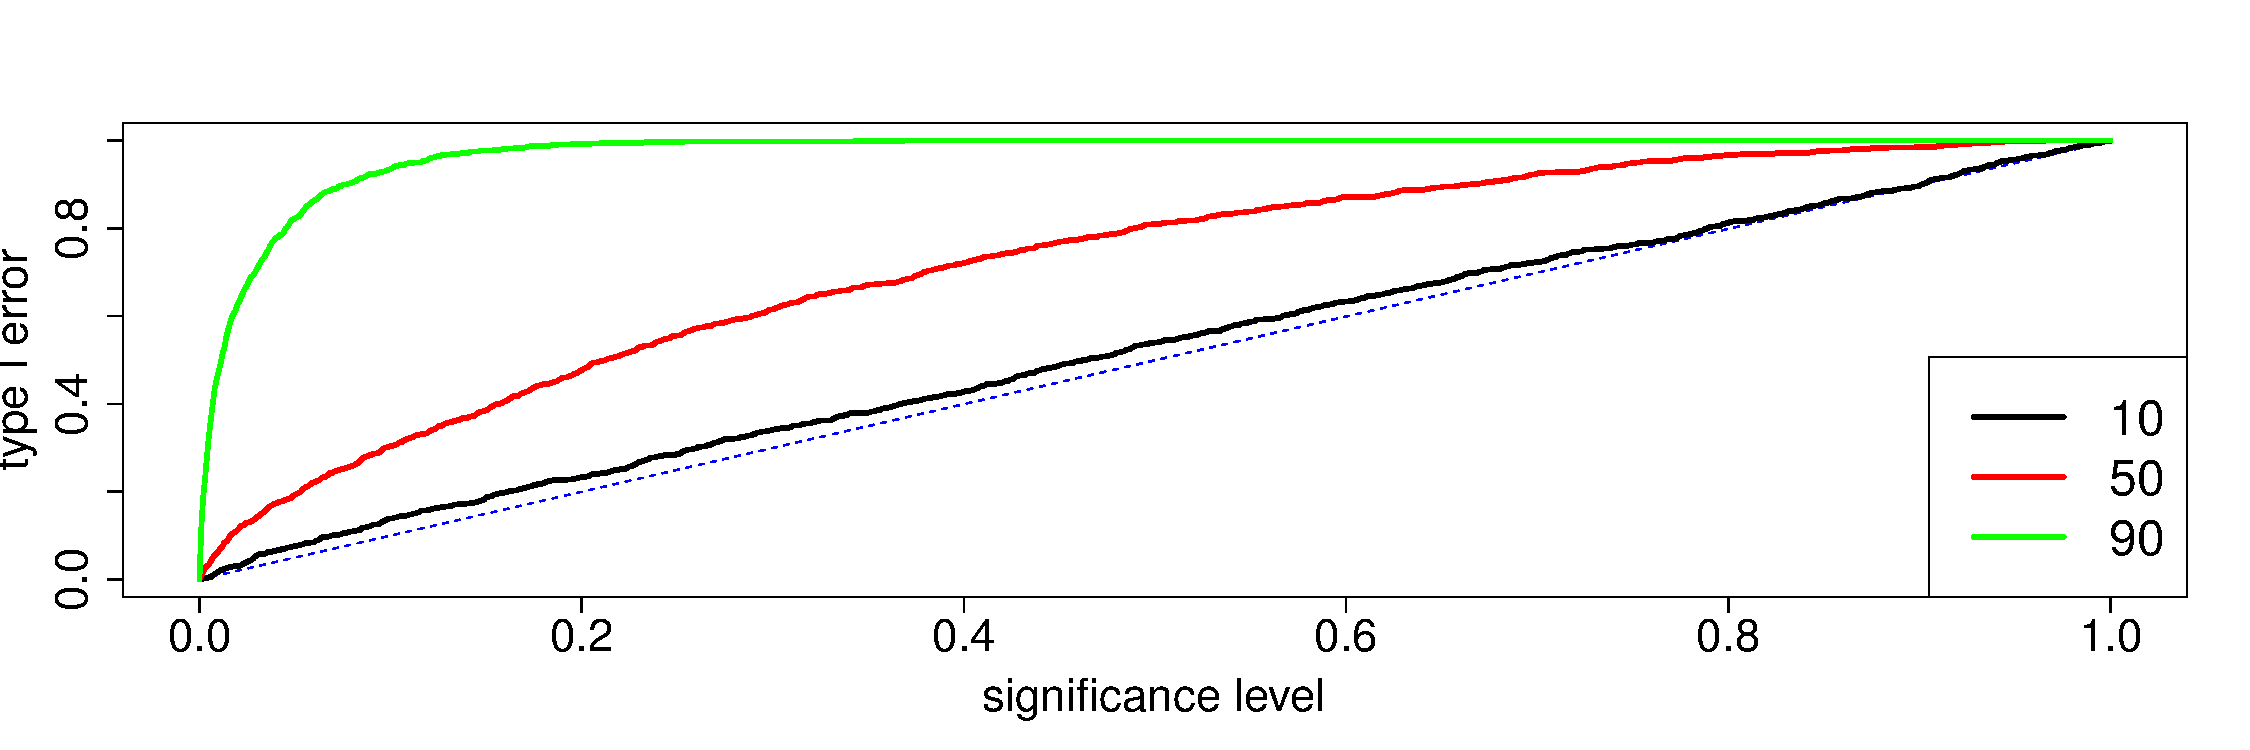
\includegraphics[width=0.7\textwidth]{img/alphaI_phi3_N100}
			\caption{Ошибка I рода}
			\label{alphaI_phi3_N100}
		\end{subfigure}
		\begin{subfigure}[t]{\textwidth}
			\centering
			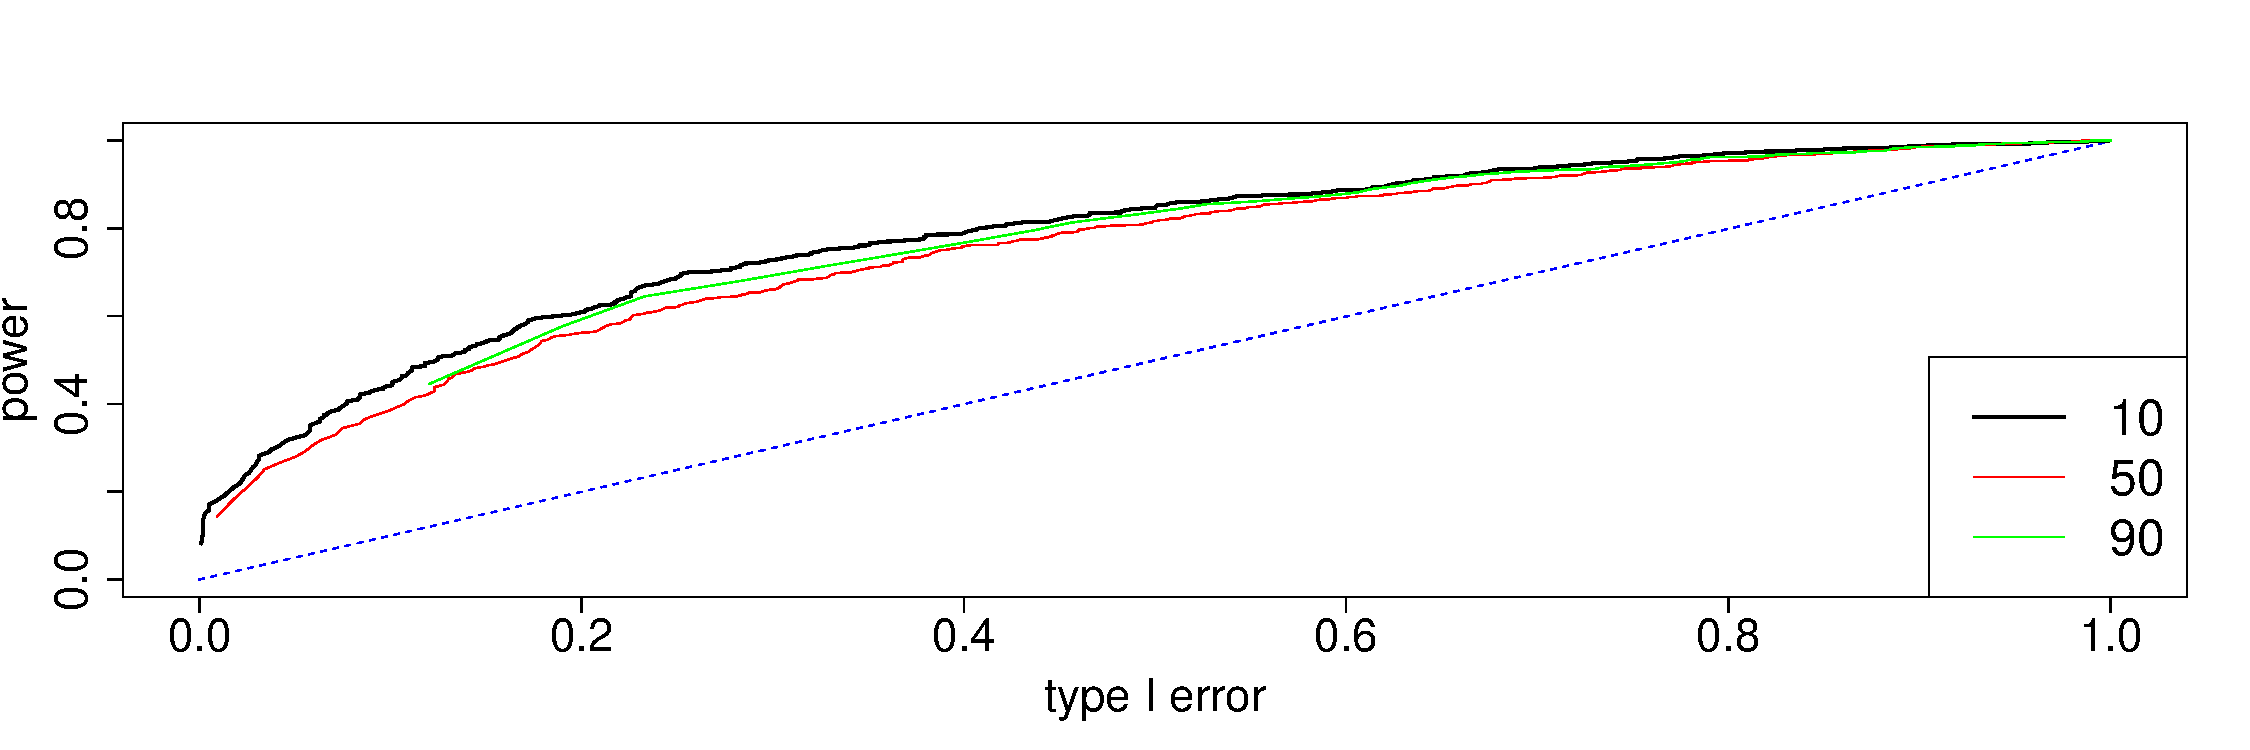
\includegraphics[width=0.7\textwidth]{img/roc_phi3_N100}
			\caption{ROC-кривая ($A=0.7$, $\omega=0.075$)}
			\label{roc_phi3_N100}
		\end{subfigure}
	\label{fig:example2}
	\caption{Пример~\ref{example2} ($\varphi=0.3$, $N=100$)}
	\end{figure}
	На рис.~\ref{alphaI_phi3_N100} изображен график ошибок первого рода. По нему видно, что, как и в примере 1, чем больше $L$, тем больше радикальность критерия. Если взглянуть на ROC-кривые на рис.~\ref{roc_phi3_N100}, то видно, что с уменьшением параметра $\varphi$ уменьшается разброс мощности критериев после поправки в зависимости от длины окна. Лучшей из рассмотренных в этом случае является $L=10$, хотя разница с $L=50$ совсем небольшая, а для $L=90$ для небольших ошибок I рода поправку сделать не удалось из-за радикальности.
\end{example}

Объяснить такое поведение радикальности в зависимости от длины окна $L$ можно теоретически: с увеличением $L$ увеличивается размер автоковариационной матрицы и тем самым увеличивается количество оцениваемых параметров, что влечет за собой большую подгонку собственных векторов к конкретной реализации шума.

\begin{example}\label{example4}
	В условиях примера~\ref{example1} рассмотрим разные частоты $\omega$ сигнала $\tS$ и зависимость упорядоченности критериев по мощности от $L$.
	\begin{figure}[h!]
		\captionsetup[subfigure]{justification=Centering}
		\begin{subfigure}[t]{\textwidth}
			\centering
			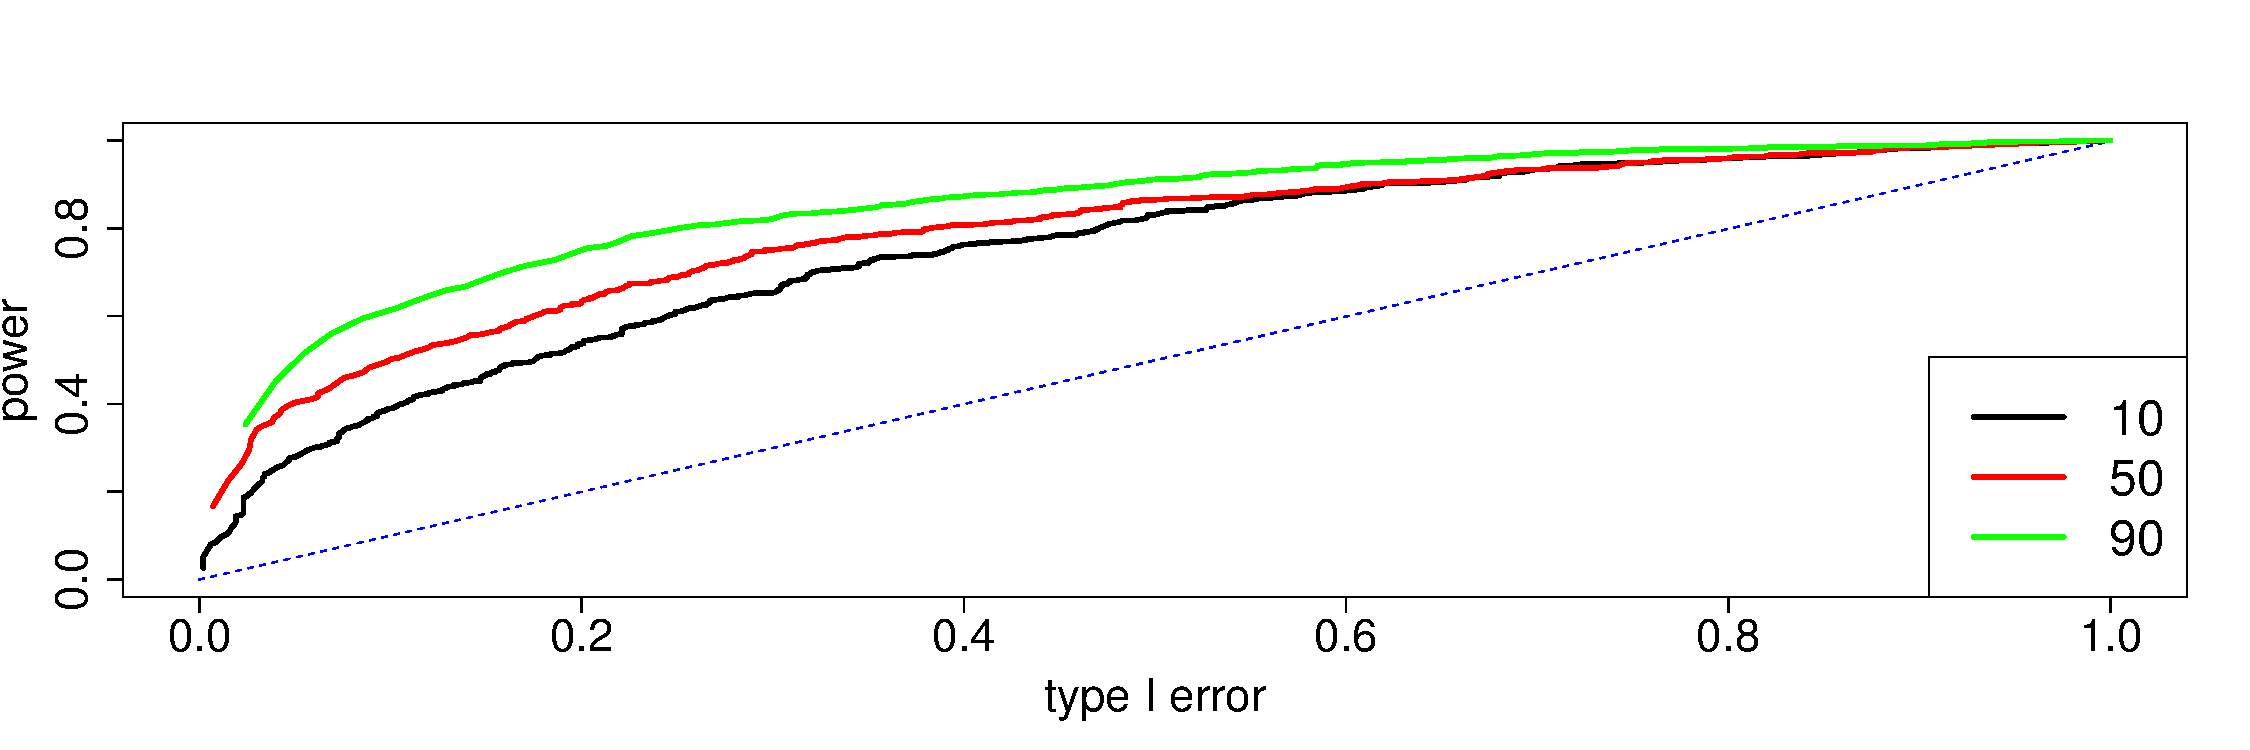
\includegraphics[width=0.7\textwidth]{img/roc_omega0175}
			\caption{ROC-кривая ($A=0.6$, $\omega=0.175$)}
			\label{roc_omega0025}
		\end{subfigure}
		\begin{subfigure}[t]{\textwidth}
			\centering
			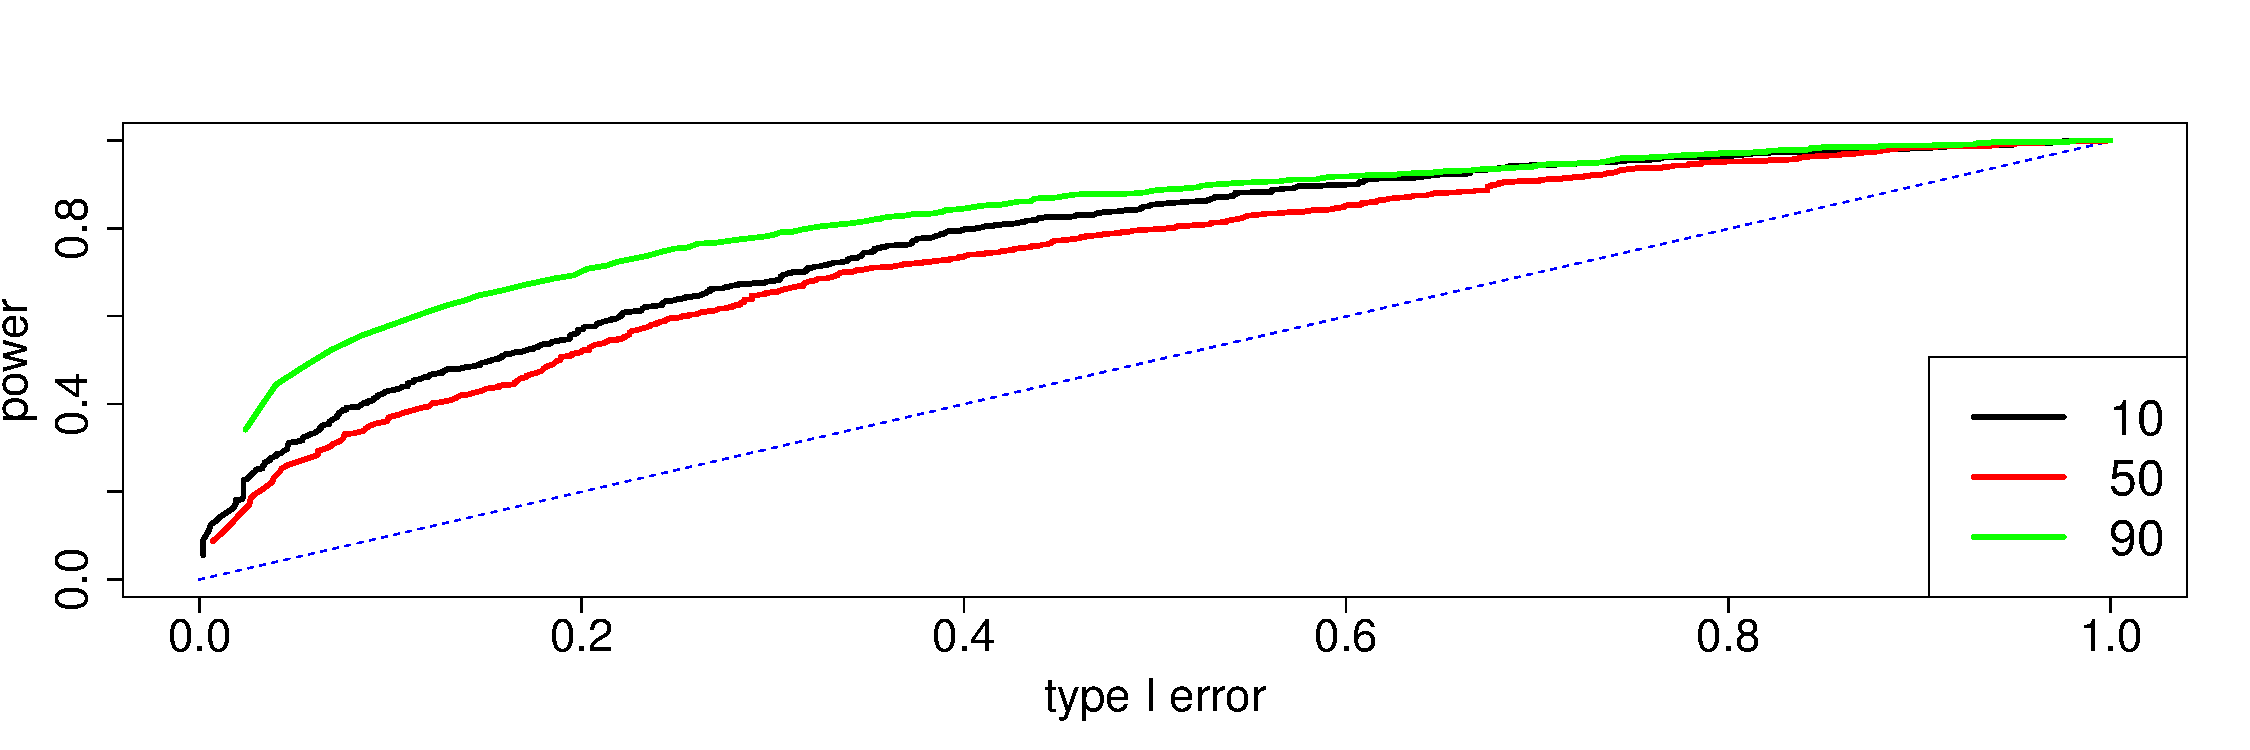
\includegraphics[width=0.7\textwidth]{img/roc_omega0025}
			\caption{ROC-кривая ($A=1.5$, $\omega=0.025$)}
			\label{roc_omega0175}
		\end{subfigure}
	\label{fig:example4}
	\caption{Пример~\ref{example4} ($\varphi=0.7$, $N=100$)}
	\end{figure}
	На рис.~\ref{roc_omega0175},~\ref{roc_omega0025} изображены ROC-кривые критериев при разных альтернативах. Видно, что упорядоченность $L$ нарушается при маленьких частотах сигнала. Если упорядочить рис.~\ref{roc_omega0175}, рис.~\ref{roc_phi7_N100} и рис.~\ref{roc_omega0025} по частоте $\omega$, то видна динамика по соотношению ROC-кривых для $L=10$ и $L=50$.
\end{example}

\begin{example}\label{example5}
	В условиях примера~\ref{example1} рассмотрим $N=100$, $200$, $500$, $1000$ и посмотрим на графики ошибок I рода и ROC-кривые при $L=10$ и $L=40$.
	\begin{figure}[h!]
		\captionsetup[subfigure]{justification=Centering}
		\begin{subfigure}[t]{\textwidth}
			\centering
			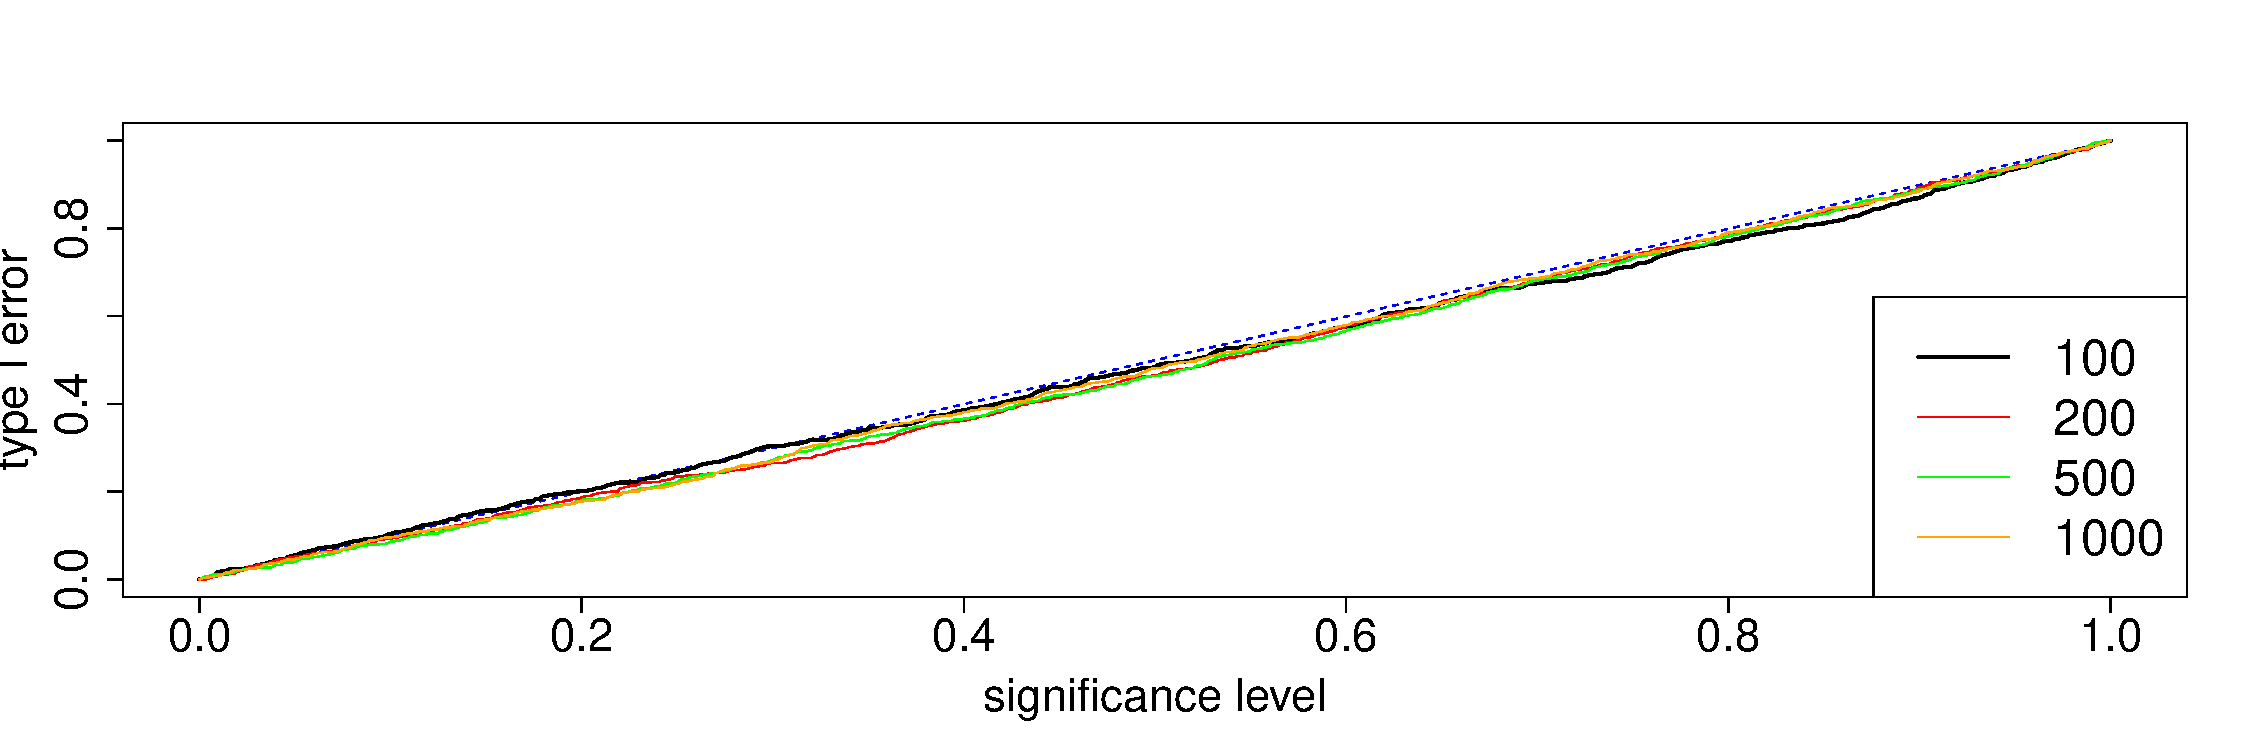
\includegraphics[width=0.7\textwidth]{img/alphaI_L10.pdf}
			\caption{Ошибка I рода ($L=10$)}
			\label{alphaI_L10}
		\end{subfigure}
		\begin{subfigure}[t]{\textwidth}
			\centering
			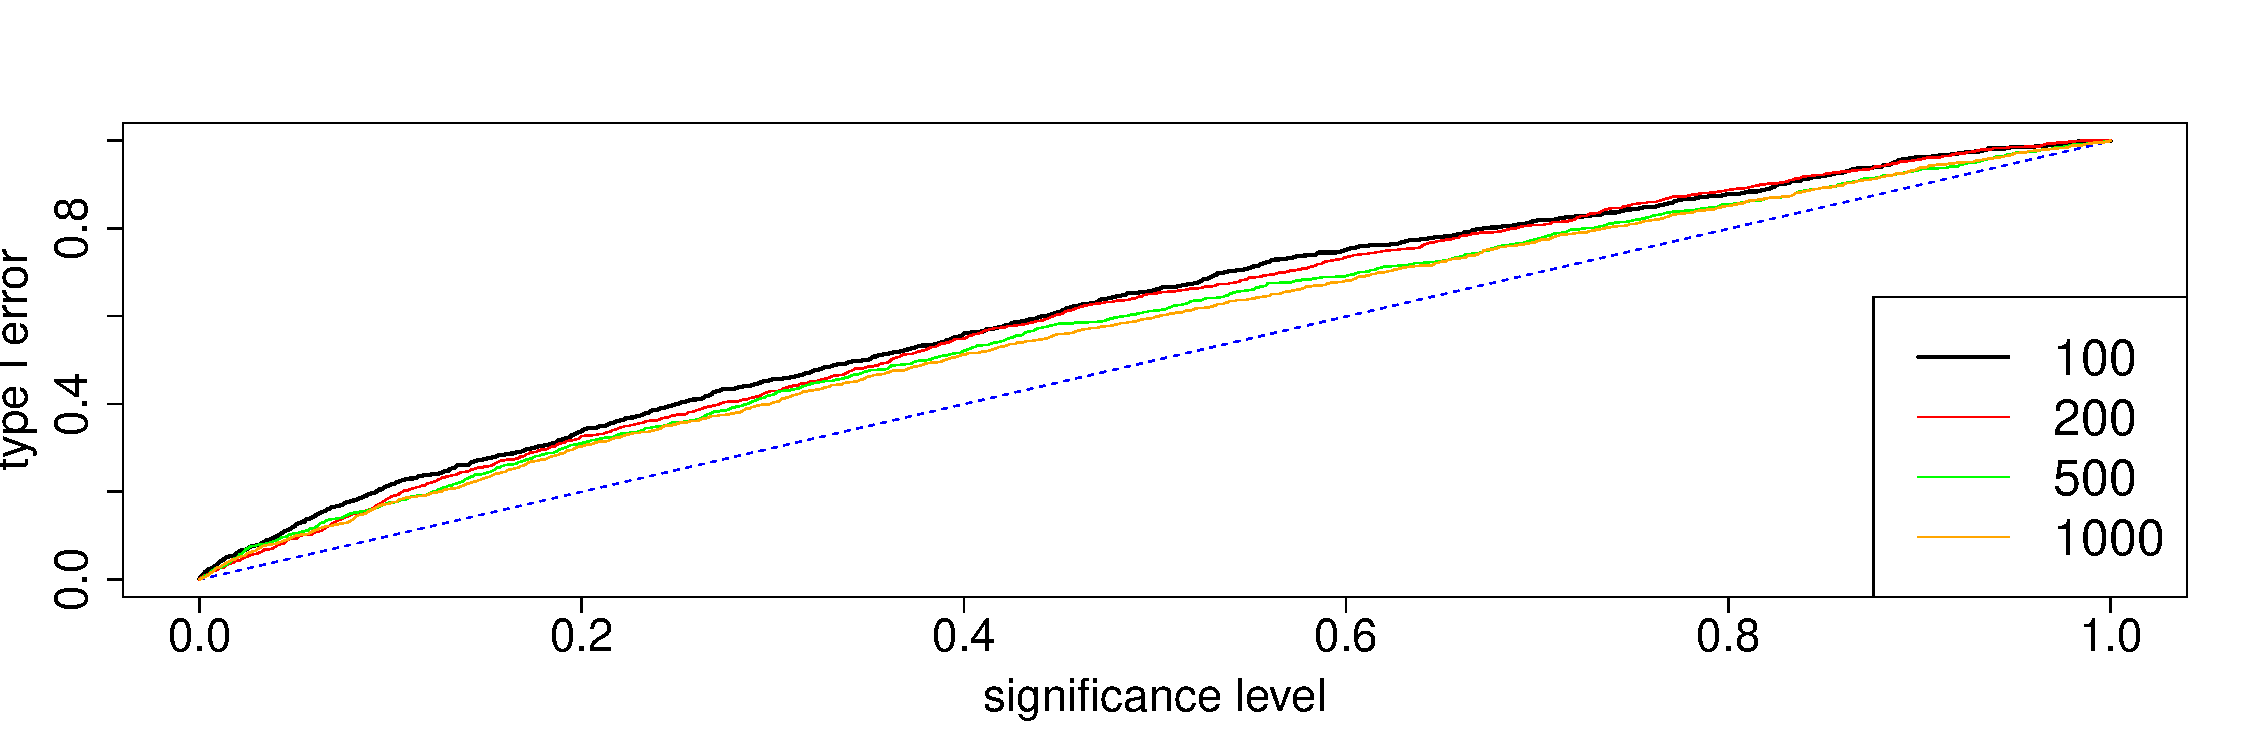
\includegraphics[width=0.7\textwidth]{img/alphaI_L40.pdf}
			\caption{Ошибка I рода ($L=40$)}
			\label{alphaI_L40}
		\end{subfigure}
		\begin{subfigure}[t]{\textwidth}
			\centering
			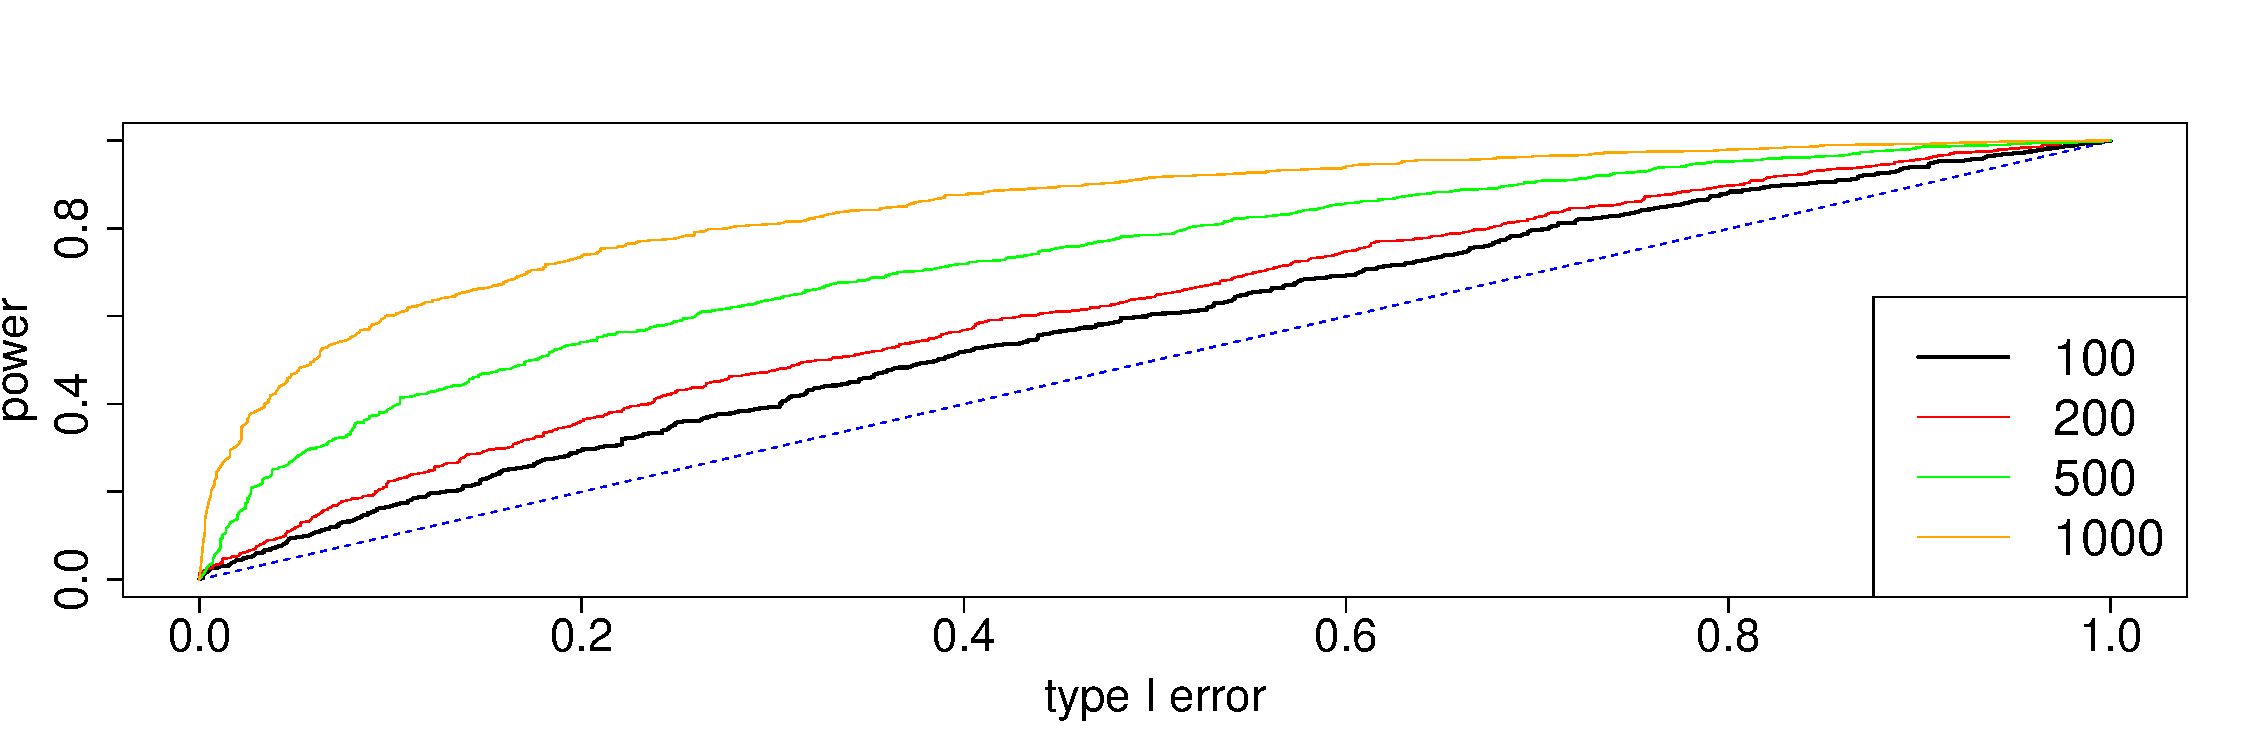
\includegraphics[width=0.7\textwidth]{img/roc_L10.pdf}
			\caption{ROC-кривая ($L=10$)}
			\label{roc_L10}
		\end{subfigure}
		\begin{subfigure}[t]{\textwidth}
			\centering
			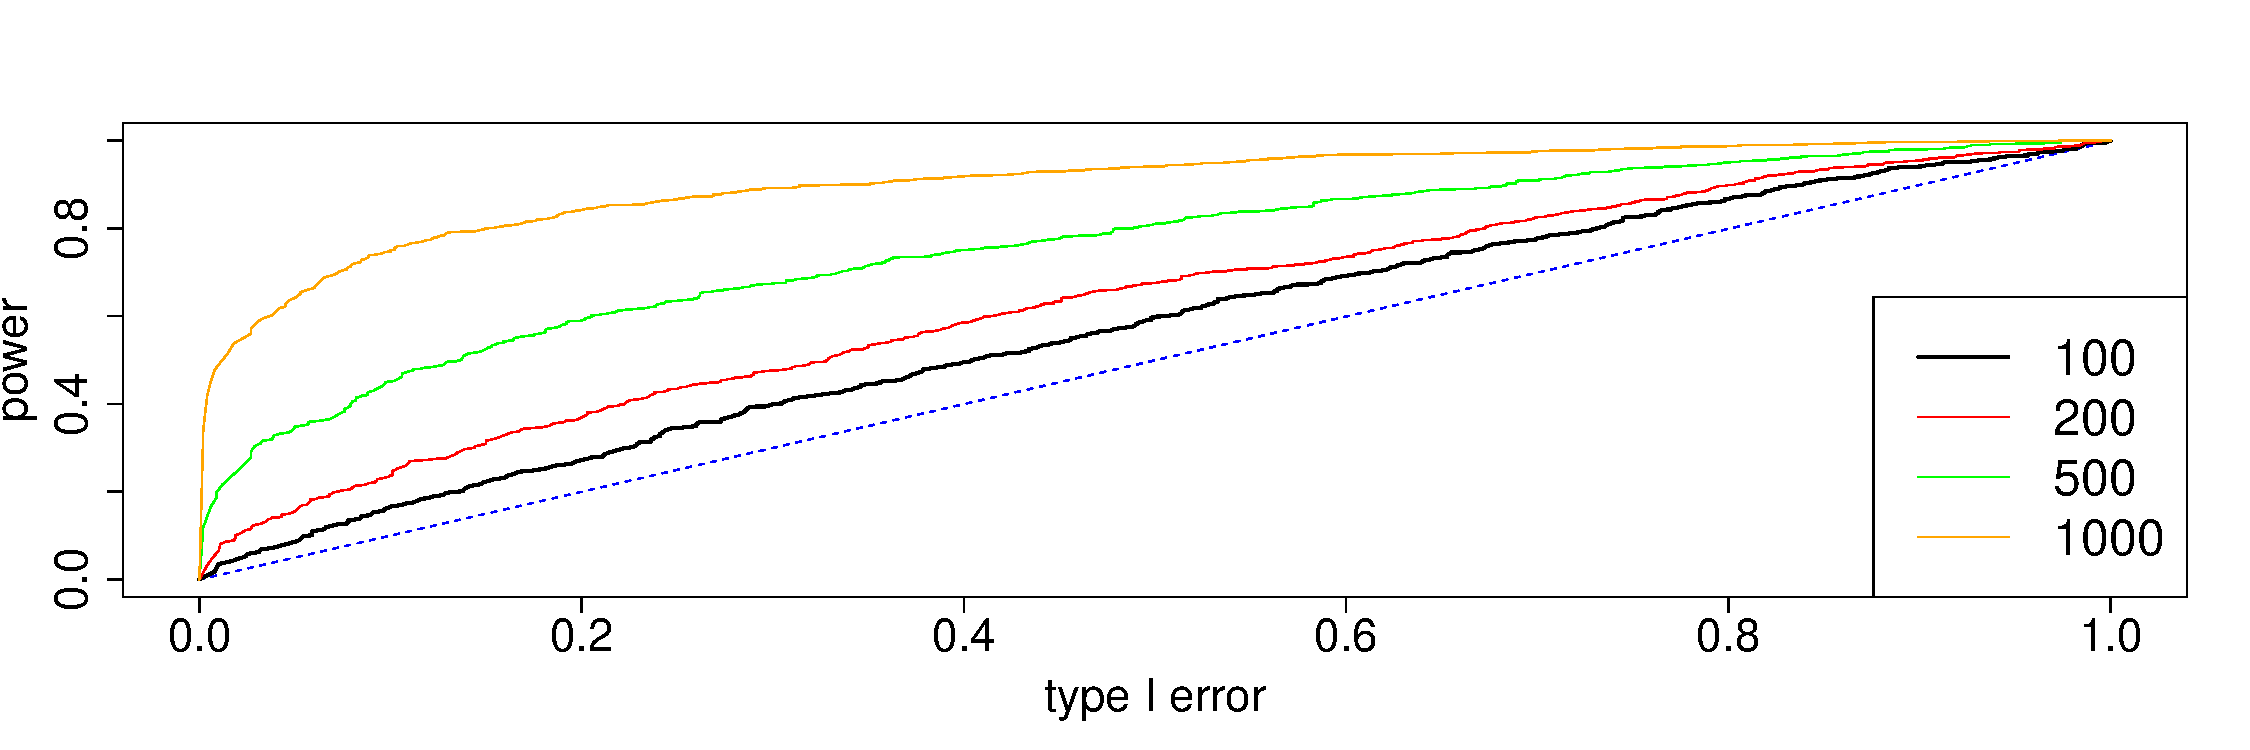
\includegraphics[width=0.7\textwidth]{img/roc_L40.pdf}
			\caption{ROC-кривая ($L=40$)}
			\label{roc_L40}
		\end{subfigure}
	\label{fig:example5}
	\caption{Пример~\ref{example5} ($\varphi=0.7$, $A=0.8$, $\omega=0.075$, разные $N$)}
	\end{figure}

	Из рис~\ref{alphaI_L10} видно, что критерий с $L=10$ примерно точный для всех $N$, а на рис.~\ref{alphaI_L40} наблюдается очень медленное уменьшение радикальности критерия с ростом $N$. По ROC-кривым на рис.~\ref{roc_L10} и~\ref{roc_L40} видна состоятельность критерия против рассмотренной альтернативы.

\end{example}

Численные эксперименты показали, что длина окна $L$, дающая максимальную мощность критерия после поправки, зависит от параметров шума, длины ряда и, главное, от частоты сигнала в альтернативной гипотезе. Поэтому при выборе длины окна возможны следующие варианты:
\begin{enumerate}
	\item При больших $N$ применение поправки, описанной в разделе~\ref{sect:correction}, является трудоемкой задачей даже для небольших $L$. Поэтому из рассмотренных примеров получено, что без поправки можно использовать MC-SSA только с $L=10$. Это нетрудозатратно, но возможна некоторая потеря в мощности.
	\item В поведении оптимальной по мощности длины окна $L$ в зависимости от параметров ряда наблюдается некоторая регулярность. Поэтому можно построить зависимость оптимальной длины окна от параметров ряда с помощью численного моделирования, оценив параметры красного шума. Однако было показано, что упорядоченность критериев по мощности зависит от частоты сигнала в альтернативе, поэтому эта рекомендация имеет практический смысл, только если есть дополнительная информация о диапазоне возможных частот в альтернативе.
\end{enumerate}

\section{Оценка параметров красного шума}\label{sect:phi_est}
До сих пор предполагалось, что параметры красного шума $\varphi$ и $\delta$ известны, но в реальных задачах редко возникает такая ситуация. В этой ситуации можно воспользоваться методом bootstrapping, который позволяет использовать оцененные параметры шума для построения критерия~\cite{Golyandina2023}. Тогда параметры оцениваются на основе исходного ряда методом максимального правдоподобия, где для нахождения начальных значений используется метод CSS~\cite{Gardner1980}.

\subsection{Искажение критерия при использовании оценок}\label{sect:mc-ssa_est}
В условиях примеров~\ref{mc-mssa_example1},~\ref{mc-mssa_example2} и~\ref{mc-mssa_example3} раздела~\ref{sect:mc-mssa_numeric_comparison} и посмотрим, насколько сильно искажается критерий MC-SSA, если оценивать параметры красного шума.
\begin{figure}[h!]
	\captionsetup[subfigure]{justification=Centering}
	\begin{subfigure}[t]{0.5\textwidth}
		\centering
		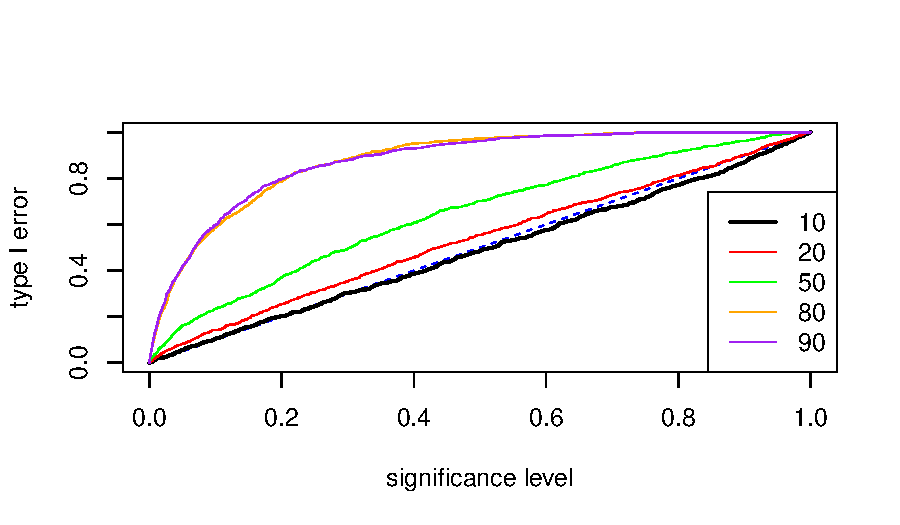
\includegraphics[width=\textwidth]{img/type1error_phi7.pdf}
		\caption{Ошибка I рода (известные параметры)}
		\label{fig:type1error_phi7}
	\end{subfigure}\hspace{\fill}
	\begin{subfigure}[t]{0.5\textwidth}
		\centering
		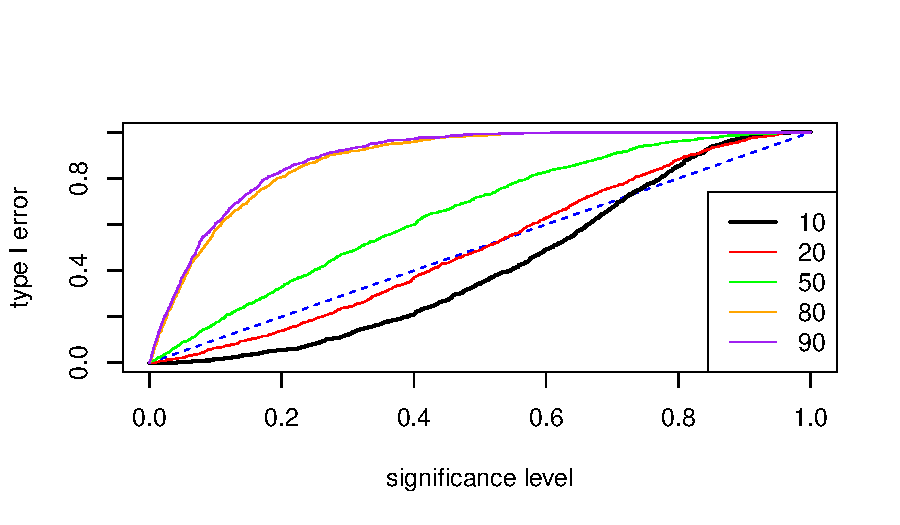
\includegraphics[width=\textwidth]{img/type1error_phi7est.pdf}
		\caption{Ошибка I рода (оцененные параметры)}
		\label{fig:type1error_phi7est}
	\end{subfigure}
	\bigskip
	\begin{subfigure}[t]{0.5\textwidth}
		\centering
		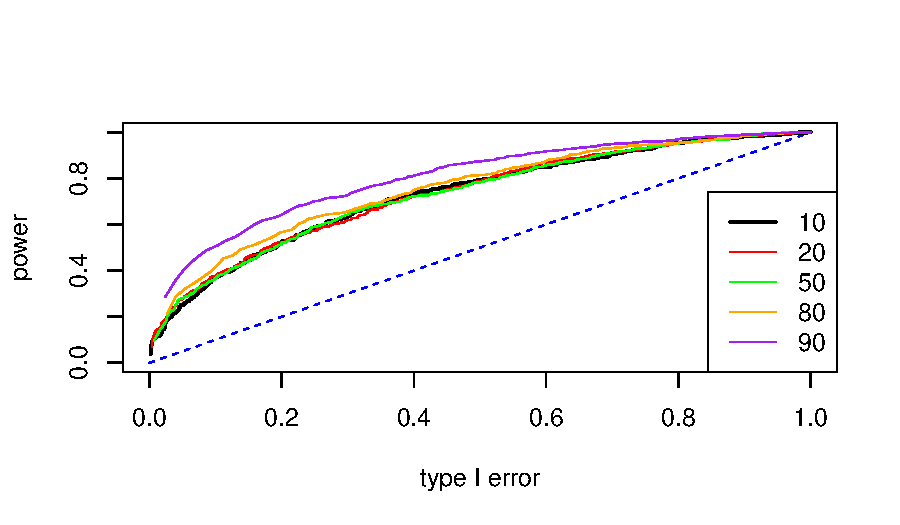
\includegraphics[width=\textwidth]{img/roc_phi7_omega0075.pdf}
		\caption{ROC-кривая (известные параметры)}
		\label{fig:roc_phi7_omega0075}
	\end{subfigure}\hspace{\fill}
	\begin{subfigure}[t]{0.5\textwidth}
		\centering
		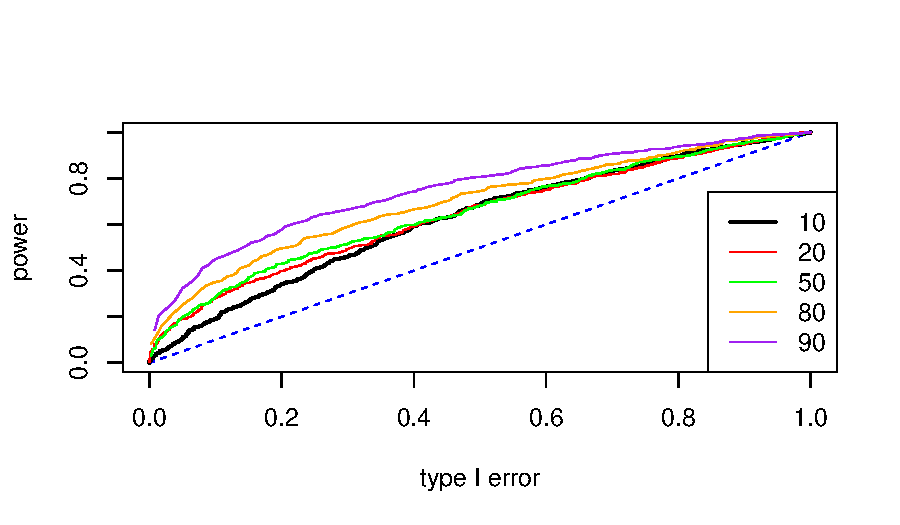
\includegraphics[width=\textwidth]{img/roc_phi7est_omega0075.pdf}
		\caption{ROC-кривая (оцененные параметры)}
		\label{fig:roc_phi7est_omega0075}
	\end{subfigure}
	\caption{Сравнение критериев ($\varphi=0.7$, $A=1$, $\omega=0.075$)}
	\label{fig:est_comp}
\end{figure}

На рис.~\ref{fig:est_comp} представлено сравнение критерия с известными и критерия с оцененными параметрами красного шума. На рис.~\ref{fig:type1error_phi7} и~\ref{fig:type1error_phi7est} изображены графики ошибок первого рода для разных длин окна, а на рис.~\ref{fig:roc_phi7_omega0075} и~\ref{fig:roc_phi7est_omega0075}~--- ROC-кривые. По ним видно, что оценка параметров снижает радикальность критерия, делая его консервативным при $L=10$ и $L=20$ для небольших $\alpha$. Мощность поправленного критерия при этом тоже снижается. Графики для остальных примеров можно найти в разделе~\ref{appendix:est_graphs}.
\begin{table}[h]
	\caption{Мощность методов для оптимальных $L$ ($\alpha^*=0.1$)}
	\label{tab:res_mc-ssa_est}
	\centering
	\begin{tabular}{|cccc|}\hline
		Пример 1 ($\varphi=0.7$, $A=1$, $\omega=0.075$) & $L$ & $\alpha_I(\alpha^*)$ & $\beta(\widetilde\alpha^*)$ \\
		\hline
		Известные параметры & 90 & 0.598 & 0.509 \\
		\hline
		Оцененные параметры & 90 & 0.605 & 0.454 \\
		\hhline{====}
		Пример 2 ($\varphi=0.3$, $A=0.7$, $\omega=0.075$) & $L$ & $\alpha_I(\alpha^*)$ & $\beta(\widetilde\alpha^*)$ \\
		\hline
		Известные параметры & 80 & 0.814 & 0.487 \\
		\hline
		Оцененные параметры & 80 & 0.839 & 0.229 \\
		\hhline{====}
		Пример 3 ($\varphi=0.7$, $A=0.4$, $\omega=0.225$) & $L$ & $\alpha_I(\alpha^*)$ & $\beta(\widetilde\alpha^*)$ \\
		\hline
		Известные параметры & 90 & 0.598 & 0.373 \\
		\hline
		Оцененные параметры & 90 & 0.605 & 0.352\\
		\hline
	\end{tabular}
\end{table}

В таблице~\ref{tab:res_mc-ssa_est} представлены результаты численного сравнения методов: длина окна, дающая наибольшую мощность, ошибка первого рода и мощность поправленного критерия при уровне значимости $\alpha^*=0.1$. Как видно из таблицы, при маленьких $\varphi$ оценка параметров довольно сильно искажает критерий: мощность для примера 2 сильно уменьшилась. Однако при больших $\varphi$ уменьшение мощности не такое значительное.

\section{Наличие мешающего сигнала}\label{sect:nuisance}
Пусть известно, что во временном ряде присутствует некоторый сигнал, но, возможно, еще есть какой-то другой. Тогда модель выглядит следующим образом:
\[
	\tX=\tF + \tS + \bfxi,
\]
где $\tF$~--- мешающий сигнал, $\tS$~--- неизвестный сигнал и $\bfxi$~--- красный шум.
Тогда проверяется следующая нулевая гипотеза с альтернативой:
\begin{align*}
	&H_0: \tS=0,\\
	&H_1: \tS \ne 0.
\end{align*}
\begin{algorithm}{MC-SSA с мешающим сигналом}\label{alg:mc-ssa_nuisance}
\begin{enumerate}
	\item Находится приближенное значение мешающего сигнала $\hat{\tF}$ и оцениваются параметры $\bfxi$ на основе остатка $\tilde\tX=\tX-\hat{\tF}$.
	\item Находятся левые векторы $P_1,\ldots,P_L$ траекторной матрицы временного ряда $\tilde\tX$, полученные из разложения~\eqref{eq:sum_decomposition}.
	\item Применяется MC-SSA к исходному ряду $\tX$ с проекцией на векторы $P_1,\ldots,P_L$, при этом суррогатными рядами являются реализации случайной величины $\boldsymbol{\eta}$:
	\[
	\boldsymbol{\eta} = \bfxi + \hat\tF.
	\]
\end{enumerate}
\end{algorithm}
Цель данной модификации алгоритма~--- устранить влияние мешающего сигнала на вектора, на которые делается проекция.

Рассмотрим вместе с алгоритмом~\ref{alg:mc-ssa_nuisance} другой вариант MC-SSA с мешающим сигналом.
\begin{algorithm}{MC-SSA с мешающим периодическим сигналом}\label{alg:mc-ssa_nuisance_periodic}
	\begin{enumerate}
		\item Находится приближенное значение мешающего сигнала $\hat{\tF}$ и оцениваются параметры $\bfxi$ на основе остатка $\tilde\tX=\tX-\hat{\tF}$.
		\item Находятся левые векторы $P_1,\ldots,P_L$ траекторной матрицы временного ряда $\tX$, полученные из разложения~\eqref{eq:sum_decomposition}.
		\item Применяется MC-SSA к исходному ряду $\tX$ с проекцией на векторы $P_1,\ldots,P_L$, при этом суррогатными рядами являются реализации случайной величины $\boldsymbol{\eta}$:
		\[
		\boldsymbol{\eta} = \bfxi + \hat\tF.
		\]
	\end{enumerate}
\end{algorithm}
\begin{remark}
	Алгоритм~\ref{alg:mc-ssa_nuisance_periodic} отличается от алгоритма~\ref{alg:mc-ssa_nuisance} тем, что рассматривается проекция на левые векторы траекторной матрицы исходного временного ряда, а не его остатка. Поэтому, поскольку для нахождения собственных векторов используется теплицево разложение, использовать в качестве мешающего сигнала для алгоритма~\ref{alg:mc-ssa_nuisance_periodic} можно только стационарный сигнал.
\end{remark}

Рассмотрим два примера мешающего сигнала в условиях примеров~\ref{mc-mssa_example1} и~\ref{mc-mssa_example2} раздела~\ref{sect:mc-mssa_numeric_comparison}.

\subsection{Периодическая компонента}\label{sect:periodic_case}
Рассмотрим в качестве мешающего сигнала синусоиду
\[
	f_n=A\cos(2\pi\omega n),\quad n=1,\ldots,N,
\]
с амплитудой $A=3$ и частотой $\omega=0.25$.

Будем выделять периодическую компоненту при помощи SSA: будем оценивать доминирующую частоту левых векторов с помощью метода \textsf{ESPRIT}~\cite[Раздел 3.1]{SSA_R} и на шаге группировки (раздел~\ref{sect:grouping}) будем брать две компоненты с наиболее близкими к $\omega$ частотами.
\begin{figure}[h!]
	\captionsetup[subfigure]{justification=Centering}
	\begin{subfigure}[t]{0.5\textwidth}
		\centering
		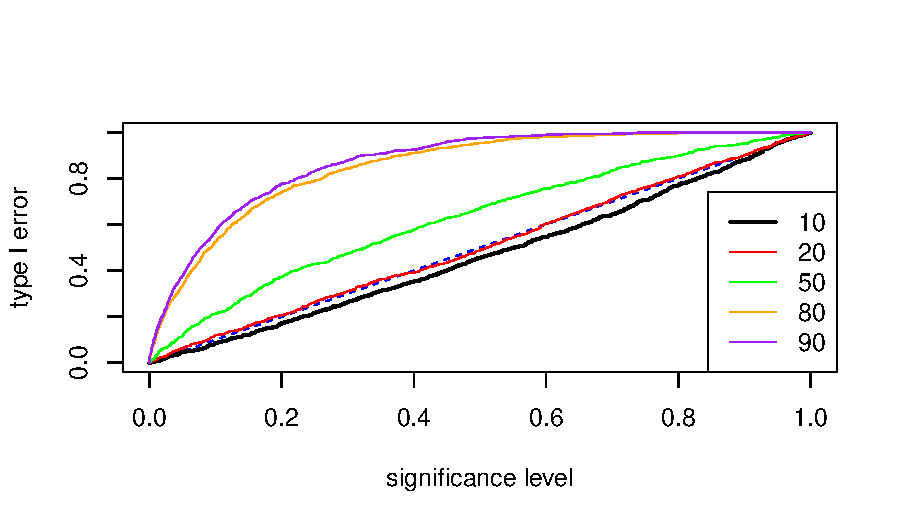
\includegraphics[width=\textwidth]{img/type1error_sin.pdf}
		\caption{Ошибка I рода}
		\label{fig:sin_type1error}
	\end{subfigure}\hspace{\fill}
	\begin{subfigure}[t]{0.5\textwidth}
		\centering
		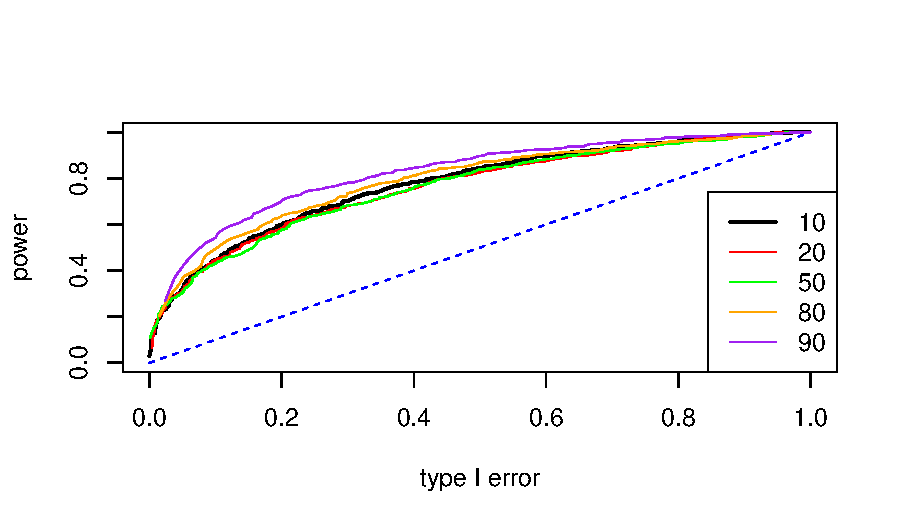
\includegraphics[width=\textwidth]{img/roc_sin.pdf}	
		\caption{ROC-кривая}
		\label{fig:sin_roc}
	\end{subfigure}
	\begin{subfigure}[t]{0.5\textwidth}
		\centering
		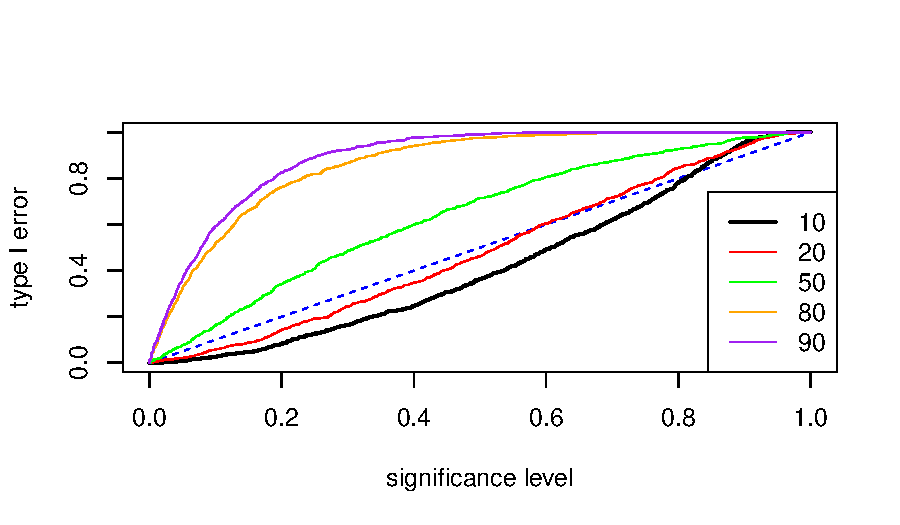
\includegraphics[width=\textwidth]{img/type1error_sin_est_noise.pdf}
		\caption{Ошибка I рода (оцененные параметры шума)}
		\label{fig:sin_est_noise_type1error}
	\end{subfigure}\hspace{\fill}
	\begin{subfigure}[t]{0.5\textwidth}
		\centering
		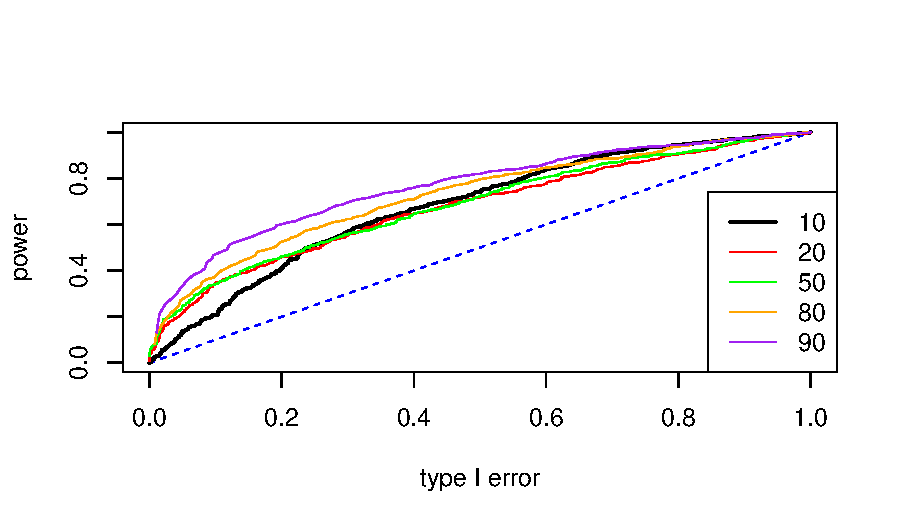
\includegraphics[width=\textwidth]{img/roc_sin_est_noise.pdf}
		\caption{ROC-кривая (оцененные параметры шума)}
		\label{fig:sin_est_noise_roc}
	\end{subfigure}
	\begin{subfigure}[t]{0.5\textwidth}
		\centering
		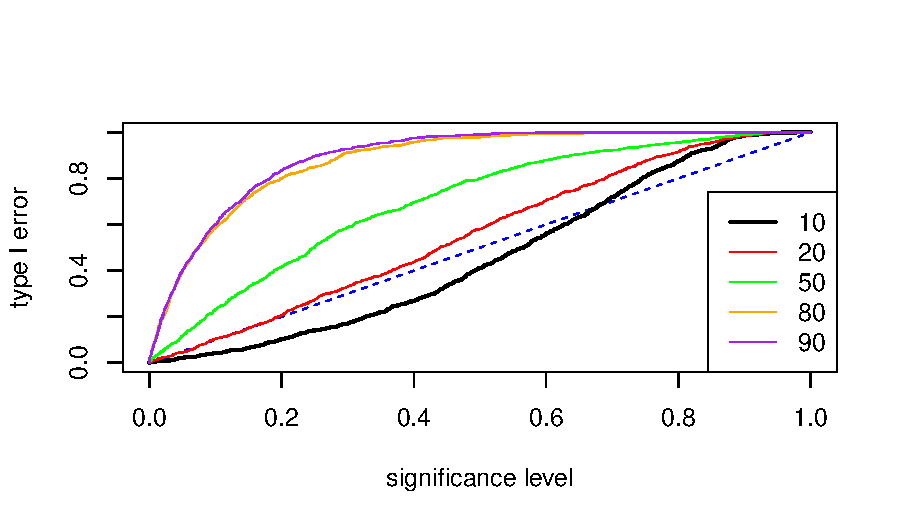
\includegraphics[width=\textwidth]{img/type1error_sin_est_noise_signal.pdf}
		\caption{Ошибка I рода (оцененный мешающий сигнал и параметры шума)}
		\label{fig:sin_est_noise_signal_type1error}
	\end{subfigure}\hspace{\fill}
	\begin{subfigure}[t]{0.5\textwidth}
		\centering
		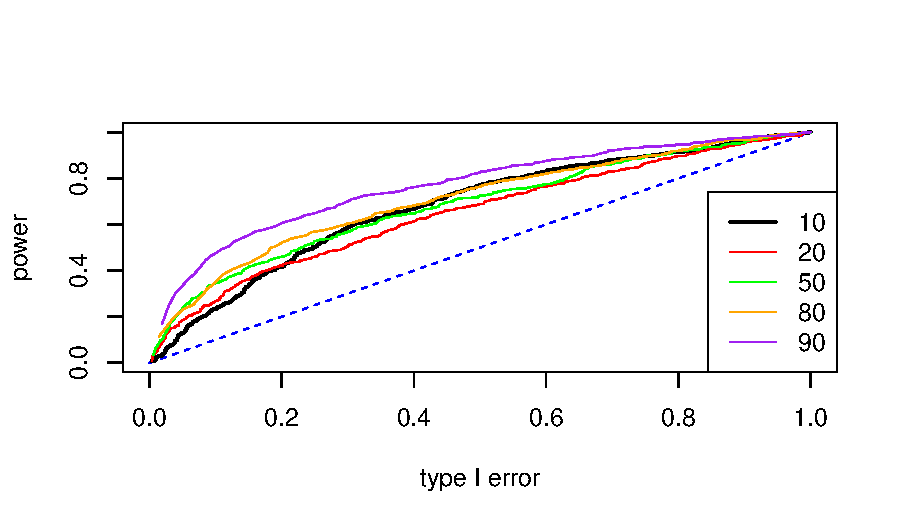
\includegraphics[width=\textwidth]{img/roc_sin_est_noise_signal.pdf}
		\caption{ROC-кривая (оцененный мешающий сигнал и параметры шума)}
		\label{fig:sin_est_noise_signal_roc}
	\end{subfigure}
	\caption{Анализ алгоритма~\ref{alg:mc-ssa_nuisance} (мешающий сигнал~--- периодика) ($\varphi=0.7$, $A=1$, $\omega=0.075$)}
	\label{fig:sin}
\end{figure}

На рис.~\ref{fig:sin} представлены графики ошибок первого рода и ROC-кривые следующих случаев алгоритма~\ref{alg:mc-ssa_nuisance}: когда мешающий сигнал и параметры шума известны точно, когда $\tF$ известен точно, но параметры шума оцениваются, и когда и мешающий сигнал, и параметры шума оцениваются. Графики ошибок первого рода на рис.~\ref{fig:sin_type1error},~\ref{fig:sin_est_noise_type1error} и~\ref{fig:sin_est_noise_signal_type1error} похожи друг на друга, а отклонение от случая, когда все известно, можно объяснить погрешностью при оценке неизвестных параметров. После применения поправки из раздела~\ref{sect:correction} критерии становятся примерно точными для любой длины окна и ROC-кривые на рис.~\ref{fig:sin_roc},~\ref{fig:sin_est_noise_roc} и~\ref{fig:sin_est_noise_signal_roc} представляют собой графики мощности этих критериев. Таким образом, наибольшая мощность во всех трех случаях достигается при $L=90$, однако заметно снижение мощности при оценивании неизвестных параметров. Графики для остальных примеров можно найти в разделе~\ref{appendix:mc-ssa_nuisance_sin_graphs}.

\begin{table}[h]
	\caption{Сравнение алгоритма~\ref{alg:mc-ssa_nuisance} и алгоритма~\ref{alg:mc-ssa_nuisance_periodic} при $\alpha^*=0.1$ ($\varphi=0.7$, $A=1$, $\omega=0.075$)}
	\label{tab:mc-ssa_nuisance_comp}
	\centering
	\begin{tabular}{|p{2.3in}c>{\centering\arraybackslash}m{1in}>{\centering\arraybackslash}m{1in}|}\hline
		Алгоритм~\ref{alg:mc-ssa_nuisance} & $L$ & $\alpha_I(\alpha^*)$ & $\beta(\widetilde\alpha^*)$ \\
		\hline
		Точная модель & 90 & 0.57 & 0.542 \\
		\hline
		Оцененные параметры шума & 90 & 0.593 & 0.48 \\
		\hline
		Оцененные параметры шума и мешающий сигнал & 90 & 0.6 & 0.475 \\
		\hhline{====}
		Алгоритм~\ref{alg:mc-ssa_nuisance_periodic} & $L$ & $\alpha_I(\alpha^*)$ & $\beta(\widetilde\alpha^*)$ \\
		\hline
		Точная модель & 90 & 0.594 & 0.532 \\
		\hline
		Оцененные параметры шума & 90 & 0.588 & 0.468 \\
		\hline
		Оцененные параметры шума и мешающий сигнал & 90 & 0.624 & 0.521 \\
		\hline
	\end{tabular}
\end{table}

В таблице~\ref{tab:mc-ssa_nuisance_comp} представлены результаты сравнения двух алгоритмов, а именно оптимальная длина окна, ошибка первого рода и мощность поправленного критерия при уровне значимости $\alpha^*=0.1$. Таблицы сравнения для остальных примеров можно найти в разделе~\ref{appendix:mc-ssa_nuisance_comp_tables}.

\subsection{Тренд}\label{sect:trend}
Отдельно рассмотрим вариант, когда мешающий сигнал~--- тренд, т.е. медленно меняющаяся компонента. Рассмотрим следующий экспоненциальный ряд:
\[
	f_n=A e^{\alpha n},\quad n=1,\ldots,N,
\]
где $A=0.2$, $\alpha=0.05$.

Выделять тренд будем с помощью SSA: поскольку в сингулярном разложении~\eqref{eq:svd} сингулярные числа, соответствующие тренду, будут самыми большими среди всех сингулярных чисел, на шаге группировки (раздел~\ref{sect:grouping}) будем брать первые $r$ элементарных компонент, где $r$~--- ранг тренда. В данном случае $r=1$.
\begin{figure}[h!]
	\captionsetup[subfigure]{justification=Centering}
	\begin{subfigure}[t]{0.5\textwidth}
		\centering
		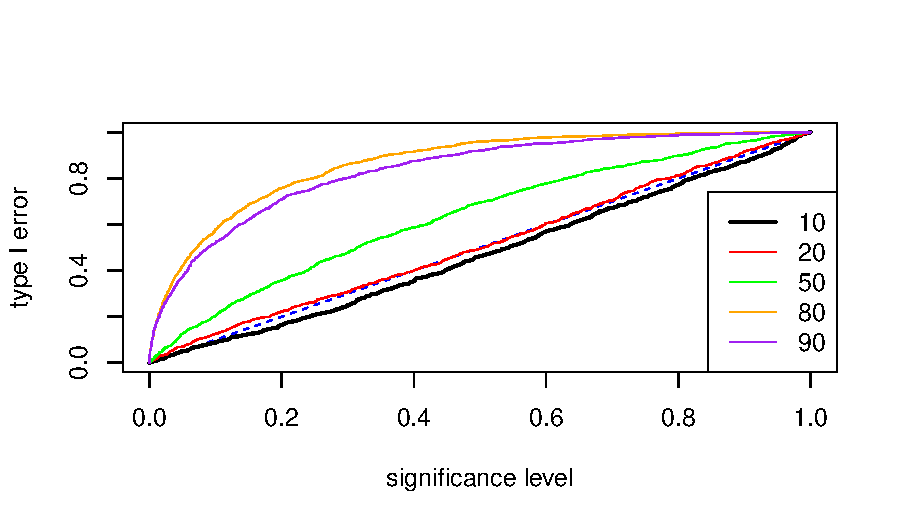
\includegraphics[width=0.95\textwidth]{img/type1error_trend.pdf}
		\caption{Ошибка I рода}
		\label{fig:trend_type1error}
	\end{subfigure}\hspace{\fill}
	\begin{subfigure}[t]{0.5\textwidth}
		\centering
		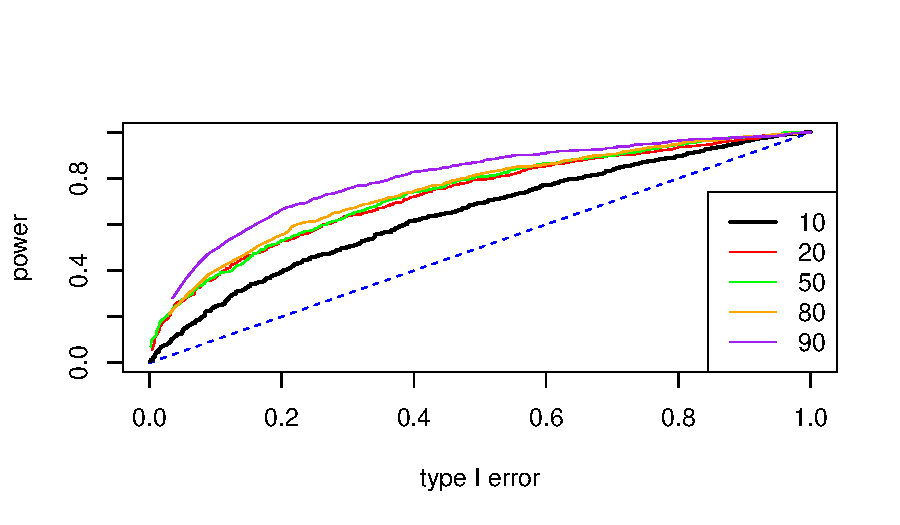
\includegraphics[width=\textwidth]{img/roc_trend.pdf}
		\caption{ROC-кривая}
		\label{fig:trend_roc}
	\end{subfigure}
	\begin{subfigure}[t]{0.5\textwidth}
		\centering
		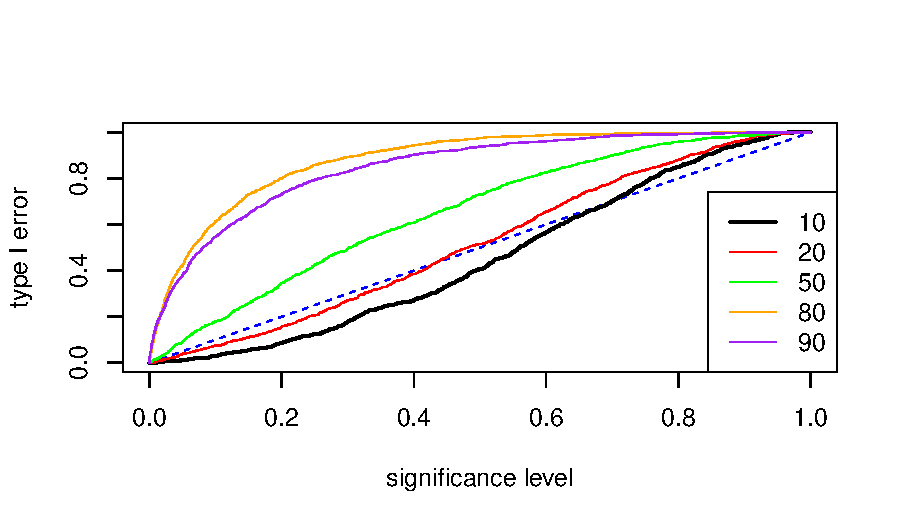
\includegraphics[width=\textwidth]{img/type1error_trend_est_noise.pdf}
		\caption{Ошибка I рода (оцененные параметры шума)}
		\label{fig:trend_est_noise_type1error}
	\end{subfigure}\hspace{\fill}
	\begin{subfigure}[t]{0.5\textwidth}
		\centering
		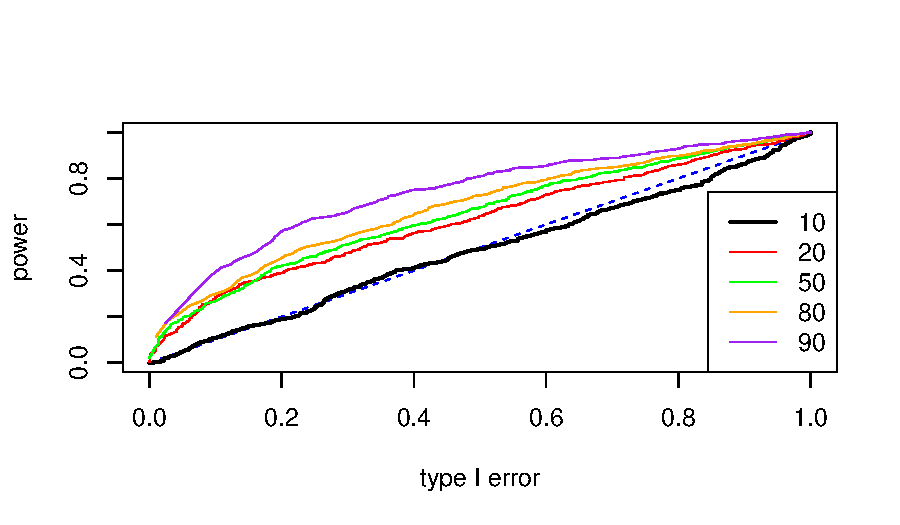
\includegraphics[width=\textwidth]{img/roc_trend_est_noise.pdf}
		\caption{ROC-кривая (оцененные параметры шума)}
		\label{fig:trend_est_noise_roc}
	\end{subfigure}
	\begin{subfigure}[t]{0.5\textwidth}
		\centering
		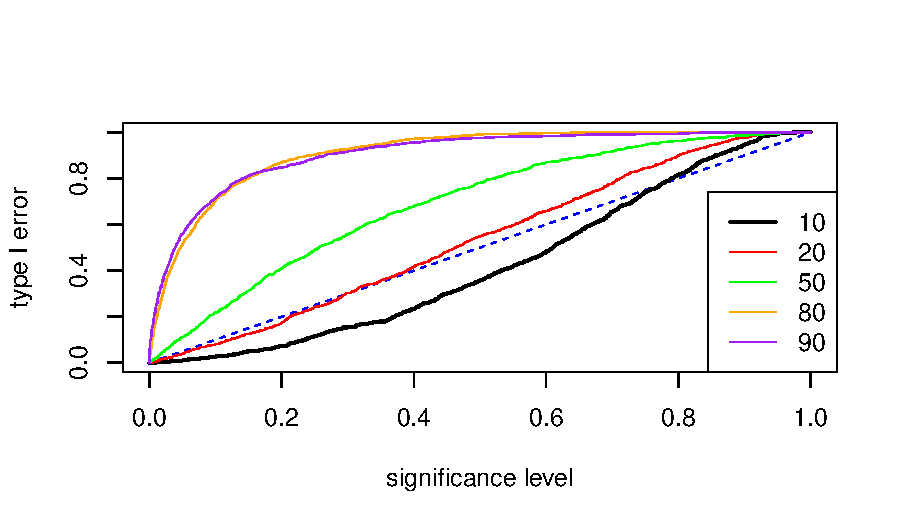
\includegraphics[width=\textwidth]{img/type1error_trend_est_noise_signal.pdf}
		\caption{Ошибка I рода (оцененный мешающий сигнал и параметры шума)}
		\label{fig:trend_est_noise_signal_type1error}
	\end{subfigure}\hspace{\fill}
	\begin{subfigure}[t]{0.5\textwidth}
		\centering
		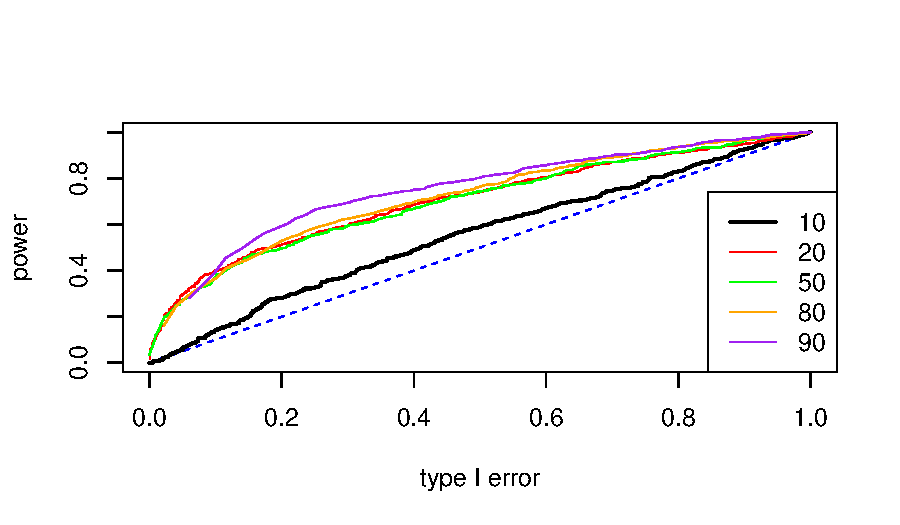
\includegraphics[width=\textwidth]{img/roc_trend_est_noise_signal.pdf}
		\caption{ROC-кривая (оцененный мешающий сигнал и параметры шума)}
		\label{fig:trend_est_noise_signal_roc}
	\end{subfigure}
	\caption{Анализ алгоритма~\ref{alg:mc-ssa_nuisance} (мешающий сигнал~--- тренд) ($\varphi=0.7$, $A=1$, $\omega=0.075$)}
	\label{fig:trend}
\end{figure}

\begin{table}[h]
	\caption{Результаты алгоритма~\ref{alg:mc-ssa_nuisance} (мешающий сигнал~--- тренд) при $\alpha^*=0.1$}
	\label{tab:mc-ssa_nuisance_trend}
	\centering
	\begin{tabular}{|p{2.8in}c>{\centering\arraybackslash}m{1in}>{\centering\arraybackslash}m{1in}|}\hline
		Пример 1 ($\varphi=0.7$, $A=1$, $\omega=0.075$) & $L$ & $\alpha_I(\alpha^*)$ & $\beta(\widetilde\alpha^*)$ \\
		\hline
		Точная модель & 90 & 0.521 & 0.501 \\
		\hline
		Оцененные параметры шума & 90 & 0.546 & 0.413 \\
		\hline
		Оцененные параметры шума и мешающий сигнал & 90 & 0.714 & 0.389 \\
		\hhline{====}
		Пример 2 ($\varphi=0.3$, $A=0.7$, $\omega=0.075$) & $L$ & $\alpha_I(\alpha^*)$ & $\beta(\widetilde\alpha^*)$ \\
		\hline
		Точная модель & 50 & 0.304 & 0.416 \\
		\hline
		Оцененные параметры шума & 50 & 0.255 & 0.223 \\
		\hline
		Оцененные параметры шума и мешающий сигнал & 50 & 0.358 & 0.243 \\
		\hhline{====}
		Пример 3 ($\varphi=0.7$, $A=0.4$, $\omega=0.225$) & $L$ & $\alpha_I(\alpha^*)$ & $\beta(\widetilde\alpha^*)$ \\
		\hline
		Точная модель & 90 & 0.521 & 0.393 \\
		\hline
		Оцененные параметры шума & 90 & 0.546 & 0.351 \\
		\hline
		Оцененные параметры шума и мешающий сигнал & 80 & 0.613 & 0.327 \\
		\hline
	\end{tabular}
\end{table}

На рис.~\ref{fig:trend} представлены графики ошибок первого рода и ROC-кривые следующих критериев: когда тренд и параметры шума $\varphi$ и $\delta$ известны точно, когда тренд известен точно, но параметры шума оцениваются, и когда и тренд, и параметры шума оцениваются. Как и в разделе~\ref{sect:periodic_case}, графики ошибок первого рода на рис.~\ref{fig:trend_type1error},~\ref{fig:trend_est_noise_type1error} и~\ref{fig:trend_est_noise_signal_type1error} сохраняют общую тенденцию при оценке неизвестных параметров. По ROC-кривым на рис.~\ref{fig:trend_roc},~\ref{fig:trend_est_noise_roc} и~\ref{fig:sin_est_noise_signal_roc} видно, что оценка неизвестных параметров снижает мощность, но оптимальной длиной окна для этого примера является в любом случае $L=90$. Графики для остальных примеров можно найти в разделе~\ref{appendix:mc-ssa_nuisance_trend_graphs}.

В таблице~\ref{tab:mc-ssa_nuisance_trend} представлены оптимальная длина окна, ошибка первого рода и мощность поправленного критерия при уровне значимости $\alpha^*=0.1$ для всех рассмотренных примеров. Как видно из таблицы, оценка тренда значительно увеличивает радикальность критерия, мощность при этом в случае $\varphi=0.7$ падает примерно на $10\%$, а в случае $\varphi=0.3$ уже довольно значительно, как и в разделе~\ref{sect:phi_est}. Также отметим, что в случае $\varphi=0.3$ критерий слишком радикальный и построить ROC-кривую для больших длин окна не удалось полностью.

\section{Применение к реальным данным}\label{sect:examples}
На рис.~\ref{Nino_ts} представлена ежемесячная температура поверхности моря в центральной тропической части Тихого океана в период с 1950 по 2024 год ($888$ месяцев). В данном регионе происходит явление под названием Эль-Ниньо, характеризующееся аномальным потеплением поверхностных вод. Эти колебания температуры оказывают заметное влияние на погодные условия во всем мире, поэтому важно изучить их поведение.
\begin{figure}[h!]
	\centering
	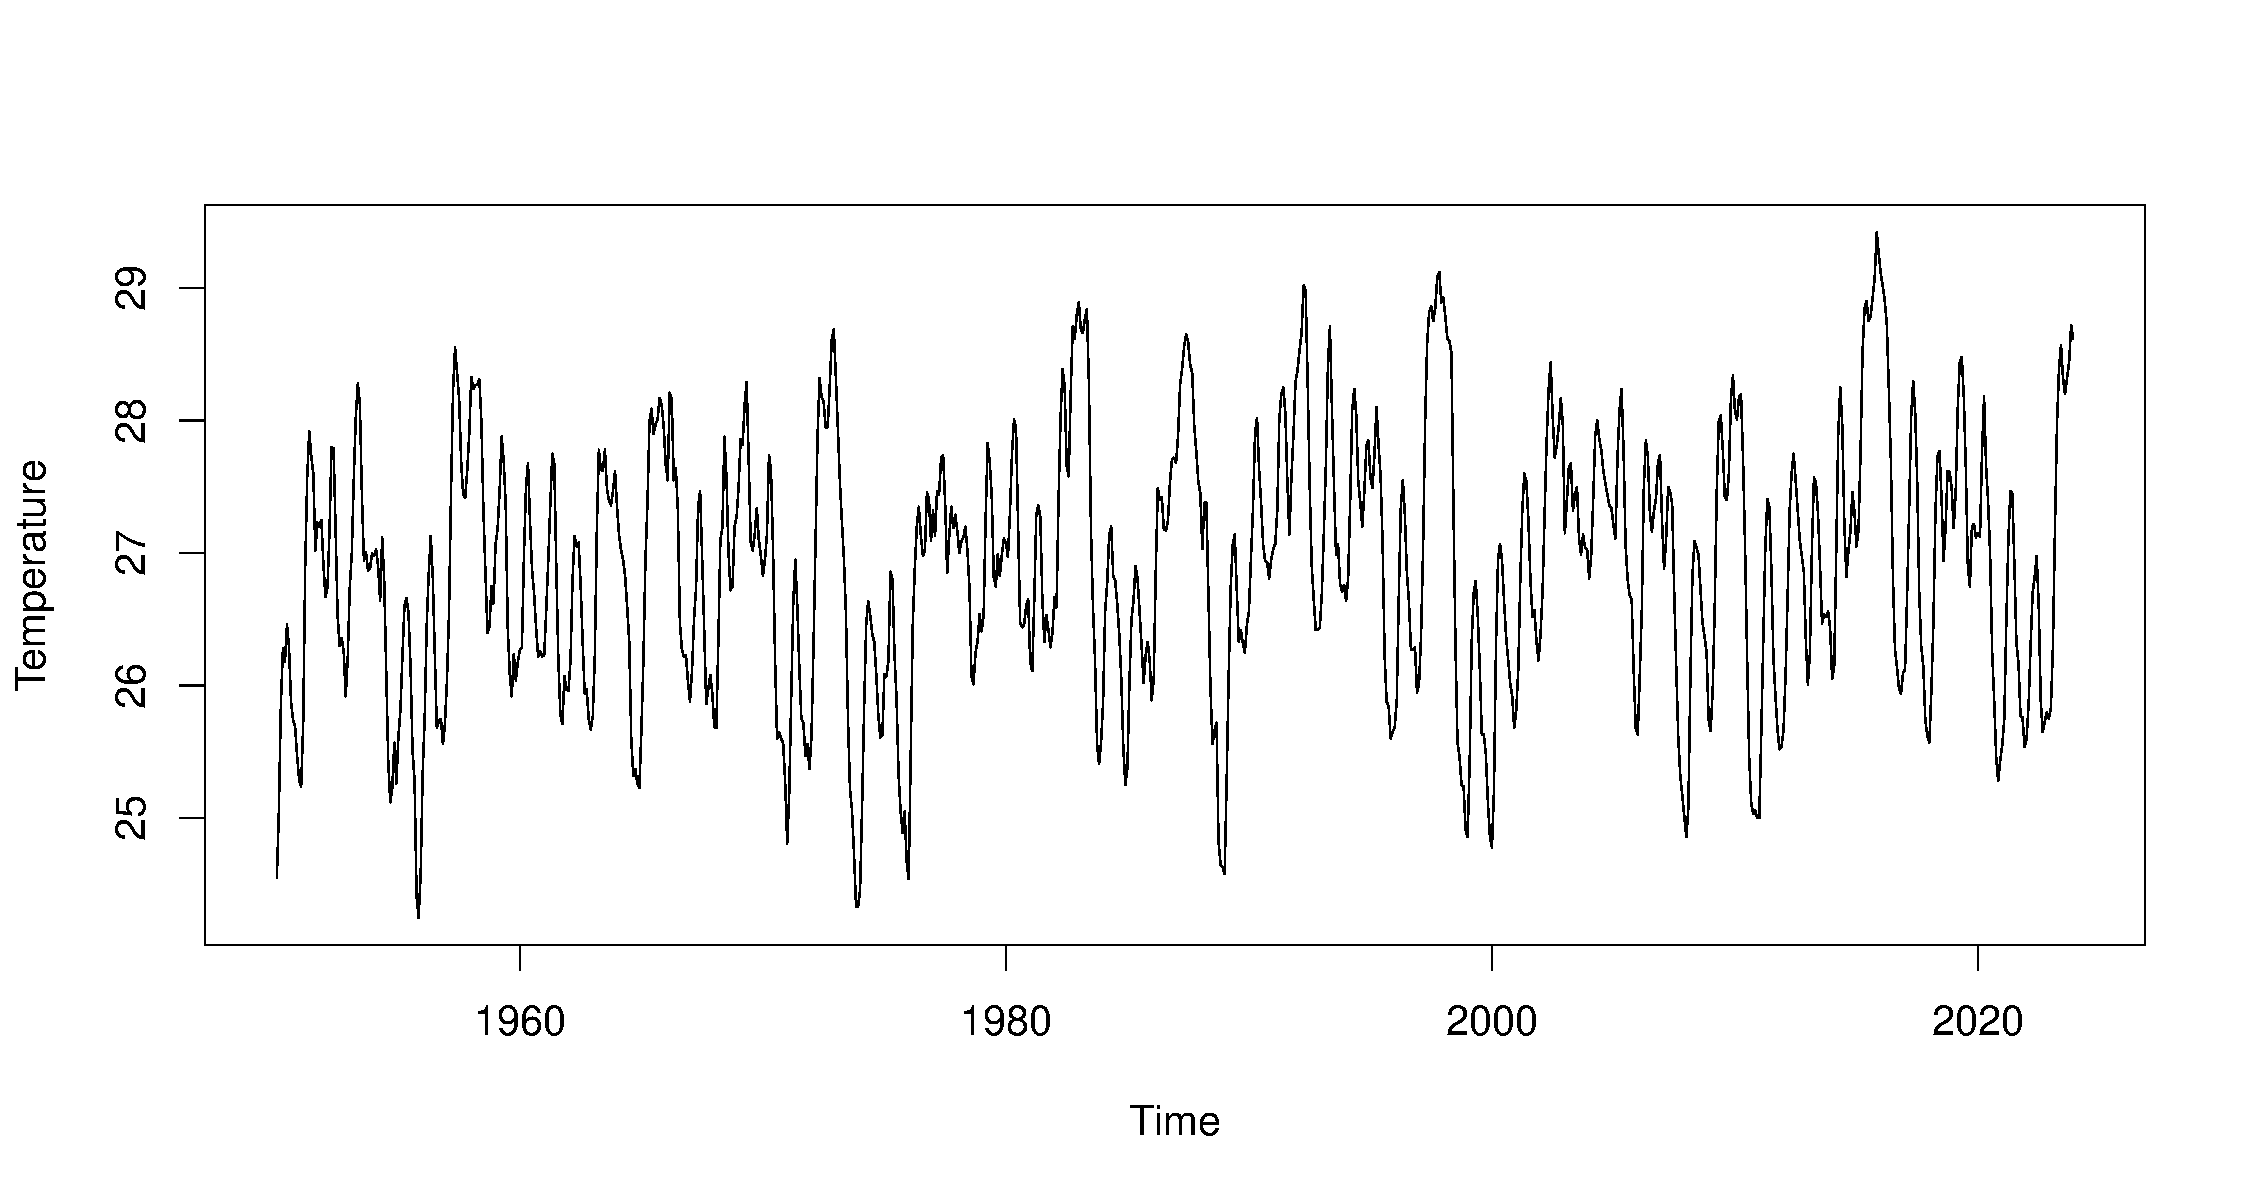
\includegraphics[width=0.8\textwidth]{img/Nino_ts.pdf}
	\caption{Температура поверхности моря в центральной тропической части Тихого океана}
	\label{Nino_ts}	
\end{figure}
\begin{figure}[h!]
	\centering
	\includegraphics[width=0.7\textwidth]{img/Nino_ssa_vectors.pdf}
	\caption{Графики собственных векторов}
	\label{Nino_ssa_vectors}	
\end{figure}

\begin{figure}[h!]
	\centering
	\includegraphics[width=0.7\textwidth]{img/Nino_ssa_paired.pdf}
	\caption{Двумерные графики собственных векторов}
	\label{Nino_ssa_paired}
\end{figure}

\begin{figure}[h!]
	\centering
	\includegraphics[width=0.8\textwidth]{img/Nino_reconstruct_trend.pdf}
	\caption{Выделенный тренд}
	\label{Nino_reconstruct_trend}
\end{figure}

Сразу заметим, что в этом временном ряде присутствует небольшой тренд, поэтому перед применением MC-SSA удалим его. Для начала воспользуемся базовым SSA с длиной окна $L=N/2=444$, как рекомендуется в~\cite{Golyandina2001}. На рис.~\ref{Nino_ssa_vectors} изображены первые 6 собственных векторов сингулярного разложения. Видно, что первый вектор соответствует тренду. Посмотрев на двумерные графики собственных векторов на рис.~\ref{Nino_ssa_paired}, видно, что вторая и третья компоненты образуют двенадцатиугольник. Это означает, что они соответствуют периодике с периодом 12~\cite{Golyandina2001}. С учетом всей полученной информации, возьмем длину окна для выделения тренда небольшой, но делящейся на период периодической компоненты для обеспечения разделимости~\cite{Golyandina2001}. На рис.~\ref{Nino_reconstruct_trend} изображен выделенный тренд при $L=120$.
\begin{figure}[h!]
	\centering
	\includegraphics[width=0.8\textwidth]{img/Nino_reconstruct_season.pdf}
	\caption{Выделенная годовая сезонность}
	\label{Nino_reconstruct_season}
\end{figure}
Для наиболее точного выделения периодической компоненты длина окна должна быть близкой к половине длины ряда и должна делиться на ее период~\cite{Golyandina2001}, поэтому применим Toeplitz SSA с длиной окна $L=444$. На рис.~\ref{Nino_reconstruct_season} изображена выделенная годовая сезонность.
\begin{figure}[h!]
	\centering
	\includegraphics[width=0.7\textwidth]{img/Nino_mcssa.pdf}
	\caption{Результат работы MC-SSA}
	\label{Nino_mcssa}
\end{figure}
\begin{figure}[h!]
	\centering
	\includegraphics[width=0.8\textwidth]{img/Nino_reconstruct_semi_annual.pdf}
	\caption{Выделенная полугодовая сезонность}
	\label{Nino_reconstruct_semi_annual}
\end{figure}

Применим поправленный MC-SSA с $L=40$ к ряду без тренда с годовой периодичностью в качестве мешающего сигнала (алгоритм~\ref{alg:mc-ssa_nuisance_periodic}). Оцененные параметры красного шума следующие: $\varphi=0.94$ и $\delta=0.305$. Получено p-value, равное $0$. На рис.~\ref{Nino_mcssa} изображены $95\%$-ные доверительные интервалы статистики $\widehat p_k$, $k=1,\ldots,L$~\eqref{eq:mc-ssa_statisctics}. Значимыми являются четыре компоненты, две компоненты, имеющие период приблизительно $6$, легко интерпретируются~---  это замеченная полугодовая сезонность. С помощью Toeplitz SSA с той же длиной окна эта сезонность была выделена, ее вид изображен на рис~\ref{Nino_reconstruct_semi_annual}. Оставшиеся значимые компоненты имеют периоды $18.16$ и $16.5$, которые довольно сложно интерпретировать.
\begin{figure}[h!]
	\centering
	\includegraphics[width=0.7\textwidth]{img/Nino_mcssa_arma12.pdf}
	\caption{Результат работы MC-SSA для модели ARMA$(1,2)$}
	\label{Nino_mcssa_arma12}
\end{figure}

Значимые векторы, интерпретация которых не представляется возможной, нельзя относить к сигналу, поскольку MC-SSA проверяет гипотезу о том, что временной ряд представляет собой реализацию красного шума, то есть возможно модель является неверной. Предположим, что рассматриваемый ряд без тренда и годовой периодичности является моделью ARMA$(p, q)$, где $p$~--- порядок авторегрессии, $q$~--- порядок скользящего среднего. Тогда наиболее подходящей моделью является ARMA$(1, 2)$~\cite{Hyndman2008}. Отметим, что красному шуму соответствует модель ARMA$(1, 0)$. Промоделировав ряд в соответствии с полученной моделью и посмотрев на доверительные интервалы статистик $\hat p_k$ на рис.~\ref{Nino_mcssa_arma12}, получаем много значимых компонент. Таким образом, неправильно выбранная модель может исказить выводы, полученные в результате применения MC-SSA, поэтому важно внимательно относиться к выбору модели при проверке гипотезы.

\conclusion
В ходе данной работы были реализованы два метода Toeplitz MSSA на языке программирования \textsf{R}. На основе численных экспериментов были сделаны следующие выводы: Sum и Block версии Toeplitz MSSA для стационарного ряда точнее выделяют гармонический сигнал, чем Basic MSSA, причем метод Toeplitz Sum MSSA для рассмотренных примеров оказался наиболее эффективным в построении автоковариационной матрицы и нахождении ее спектрального разложения.

На основе методов Sum и Block Toeplitz MSSA были реализованы модификации критерия MC-MSSA. Было получено, что во всех рассмотренных примерах метод\linebreak Toeplitz Sum MC-MSSA с проекцией на левые векторы дает самый мощный критерий, причем не слишком радикальный. Помимо этого, он численно эффективнее по сравнению с другими модификациями MC-MSSA. Поэтому этот метод более предпочтителен, чем метод Block, что важно ввиду его простоты в реализации и структуры, подходящей под пакет \textsf{Rssa}~\cite{Rssa}.

Проведено численное сравнение MC-SSA с другими критериями проверяющими гипотезу об отсутствии сигнала в красном шуме. Получено, что MC-SSA намного мощнее других критериев, особенно при малых частотах сигнала. Учитывая вычислительную трудоемкость метода, этот результат показывает, что она оправдана.

Была исследована зависимость радикальности и мощности MC-SSA от длины окна, однако оказалось, что длина окна, дающая максимальную мощность критерия после поправки, зависит от частоты сигнала в альтернативной гипотезе. Поэтому рекомендации по выбору параметра были даны только в общем виде.

Также было исследовано поведение MC-SSA в случае оценивании неизвестных параметров красного шума на основе исходного временного ряда. Получено, что степень искажения критерия зависит от параметра авторегрессии, чем он меньше, тем больше уменьшение мощности метода. Помимо оценки параметров было реализовано два алгоритма MC-SSA с мешающим сигналом и были разобраны два варианта мешающего сигнала. Для каждого примера были рассмотрены три случая: когда мешающий сигнал и параметры красного шума известны точно, когда параметры шума оцениваются, и когда вместе с параметрами оценивается мешающий сигнал.

При анализе алгоритмов была выявлена и сформулирована проблема применения поправки, делающей радикальный критерий точным, для критериев, использующих суррогатные данные. На основе этого было показано, что радикальность критерия приводит к существенному увеличению численных затрат, в связи с чем при сравнении критериев нужно учитывать не только мощность, но и радикальность, выбирая менее радикальные критерии.

В дальнейшем предполагается оптимизировать реализацию метода Toeplitz Sum MSSA, расширить набор примеров мешающих сигналов, а также выработать более общие рекомендации по выбору оптимальной длины окна.

\bibliographystyle{ugost2008}
\bibliography{diploma}

\appendix

\chapter{Графики}
\section{Численное сравнение модификаций MC-MSSA}\label{appendix:mc-mssa_graphs}
Здесь приведены графики к разделу~\ref{sect:mc-mssa_numeric_comparison} основного текста.

\subsubsection{$\varphi=0.3$, $\omega=0.075$}
\begin{figure}[h!]
	\captionsetup[subfigure]{justification=Centering}
	\begin{subfigure}[t]{0.5\textwidth}
		\centering
		\includegraphics[width=0.9\textwidth]{img/type1error_sum_ev_phi3.pdf}
		\caption{Ошибка I рода (Sum)}
		\label{fig:sum_ev_phi3}
	\end{subfigure}\hspace{\fill}
	\begin{subfigure}[t]{0.5\textwidth}
		\centering
		\includegraphics[width=0.9\textwidth]{img/type1error_block_ev_phi3.pdf}
		\caption{Ошибка I рода (Block)}
	\end{subfigure}
	\bigskip
	\begin{subfigure}[t]{0.5\textwidth}
		\centering
		\includegraphics[width=0.9\textwidth]{img/roc_sum_ev_phi3_omega0075.pdf}
		\caption{ROC-кривая (Sum)}
	\end{subfigure}\hspace{\fill}
	\begin{subfigure}[t]{0.5\textwidth}
		\centering
		\includegraphics[width=0.9\textwidth]{img/roc_block_ev_phi3_omega0075.pdf}
		\caption{ROC-кривая (Block)}
	\end{subfigure}
	\caption{Сравнение методов с проекцией на левые векторы ($\varphi=0.3$, $A=0.5$, $\omega=0.075$)}
	\label{fig:sum_block_ev_phi3}
\end{figure}

\begin{figure}[h!]
	\captionsetup[subfigure]{justification=Centering}
	\begin{subfigure}[t]{0.5\textwidth}
		\centering
		\includegraphics[width=0.9\textwidth]{img/type1error_sum_fa_phi3.pdf}
		\caption{Ошибка I рода (Sum)}
	\end{subfigure}\hspace{\fill}
	\begin{subfigure}[t]{0.5\textwidth}
		\centering
		\includegraphics[width=0.9\textwidth]{img/type1error_block_fa_phi3.pdf}
		\caption{Ошибка I рода (Block)}
	\end{subfigure}
	\bigskip
	\begin{subfigure}[t]{0.5\textwidth}
		\centering
		\includegraphics[width=0.9\textwidth]{img/roc_sum_fa_phi3_omega0075.pdf}
		\caption{ROC-кривая (Sum)}
	\end{subfigure}\hspace{\fill}
	\begin{subfigure}[t]{0.5\textwidth}
		\centering
		\includegraphics[width=0.9\textwidth]{img/roc_block_fa_phi3_omega0075.pdf}
		\caption{ROC-кривая (Block)}
	\end{subfigure}
	\caption{Сравнение методов с проекцией на правые векторы ($\varphi=0.3$, $A=0.5$, $\omega=0.075$)}
	\label{fig:sum_block_fa_phi3}
\end{figure}

На рис.~\ref{fig:sum_block_ev_phi3} изображены графики ошибок первого рода и ROC-кривые методов Sum и Block с проекцией на левые векторы, а на рис.~\ref{fig:sum_block_fa_phi3}~--- на правые векторы. Как видно по рисункам, при уменьшении параметра $\varphi$, во-первых, увеличивается радикальность критериев для любой длины окна, а во-вторых уменьшается разброс мощности после поправки. Отметим, что наименее радикальным критерием среди рассмотренных является Sum с проекцией на левые векторы (рис.~\ref{fig:sum_ev_phi3}).

\subsubsection{$\varphi=0.7$, $\omega=0.225$}
\begin{figure}[h!]
	\captionsetup[subfigure]{justification=Centering}
	\begin{subfigure}[t]{\textwidth}
		\centering
		\includegraphics[width=0.7\textwidth]{img/roc_block_ev_omega0225.pdf}
		\caption{Проекция на левые векторы}
	\end{subfigure}\hspace{\fill}
	\begin{subfigure}[t]{\textwidth}
		\centering
		\includegraphics[width=0.7\textwidth]{img/roc_block_fa_omega0225.pdf}
		\caption{Проекция на правые векторы}
	\end{subfigure}
	\caption{ROC-кривые метода Block ($\varphi=0.7$, $A=0.4$, $\omega=0.225$)}
	\label{fig:block_omega0225}
\end{figure}
\begin{figure}[h!]
	\captionsetup[subfigure]{justification=Centering}
	\begin{subfigure}[t]{\textwidth}
		\centering
		\includegraphics[width=0.7\textwidth]{img/roc_sum_ev_omega0225.pdf}
		\caption{Проекция на левые векторы}
	\end{subfigure}
	\begin{subfigure}[t]{\textwidth}
		\centering
		\includegraphics[width=0.7\textwidth]{img/roc_sum_fa_omega0225.pdf}
		\caption{Проекция на правые векторы}
	\end{subfigure}
	\caption{ROC-кривые метода Sum ($\varphi=0.7$, $A=0.4$, $\omega=0.225$)}
	\label{fig:sum_omega0225}
\end{figure}

На рис.~\ref{fig:sum_omega0225},~\ref{fig:block_omega0225} изображены ROC-кривые критериев, графики ошибок первого рода можно найти в разделе~\ref{sect:mc-mssa_numeric_comparison}. Если сравнить получившиеся графики с графиками на рис~\ref{fig:sum_fa_r},~\ref{fig:sum_fa_r},~\ref{fig:block_ev_r} и~\ref{fig:block_fa_r} из раздела~\ref{sect:mc-mssa_numeric_comparison}, видно, что с ростом частоты сигнала в альтернативе увеличивается различие в мощности критериев в зависимости от параметра $L$.

\section{Искажение критерия при использовании оценок}\label{appendix:est_graphs}
Здесь приведены графики к разделу~\ref{sect:mc-ssa_est} основного текста.
\subsubsection{$\varphi=0.3$, $\omega=0.075$}
\begin{figure}[h!]
	\captionsetup[subfigure]{justification=Centering}
	\begin{subfigure}[t]{0.5\textwidth}
		\centering
		\includegraphics[width=\textwidth]{img/type1error_phi3.pdf}
		\caption{Ошибка I рода (известные параметры)}
		\label{fig:type1error_phi3}
	\end{subfigure}\hspace{\fill}
	\begin{subfigure}[t]{0.5\textwidth}
		\centering
		\includegraphics[width=\textwidth]{img/type1error_phi3est.pdf}
		\caption{Ошибка I рода (оцененные параметры)}
		\label{fig:type1error_phi3est}
	\end{subfigure}
	\bigskip
	\begin{subfigure}[t]{0.5\textwidth}
		\centering
		\includegraphics[width=\textwidth]{img/roc_phi3_omega0075.pdf}
		\caption{ROC-кривая (известные параметры)}
		\label{fig:roc_phi3_omega0075}
	\end{subfigure}\hspace{\fill}
	\begin{subfigure}[t]{0.5\textwidth}
		\centering
		\includegraphics[width=\textwidth]{img/roc_phi3est_omega0075.pdf}
		\caption{ROC-кривая (оцененные параметры)}
		\label{fig:roc_phi3est_omega0075}
	\end{subfigure}
	\caption{Влияние оценки параметров на критерий ($\varphi=0.3$, $A=0.7$, $\omega=0.075$)}
	\label{fig:phi3est}
\end{figure}

На рис.~\ref{fig:phi3est} приведено сравнение критерия с известными и критерия с оцененными параметрами красного шума. По графикам ошибок первого рода на рис.~\ref{fig:type1error_phi3} и~\ref{fig:type1error_phi3est} видно, что для длины окна $L=10$ критерий при оценивании параметров шума становится консервативным при $\alpha<0.6$, а для $L=20$ критерий становится примерно точным при небольших $\alpha$. При остальных $L$ оценка параметров сильно на радикальность критерия не повлияла. Если взглянуть на ROC-кривые методов на рис.~\ref{fig:roc_phi3_omega0075} и~\ref{fig:roc_phi3est_omega0075}, можно заметить значительное снижение мощности поправленного критерия для всех длин окна.

\subsubsection{$\varphi=0.7$, $\omega=0.225$}
\begin{figure}[h!]
	\captionsetup[subfigure]{justification=Centering}
	\begin{subfigure}[t]{\textwidth}
		\centering
		\includegraphics[width=0.7\textwidth]{img/roc_phi7_omega0225.pdf}
		\caption{ROC-кривая (известные параметры)}
		\label{fig:roc_phi7_omega0225}
	\end{subfigure}
	\begin{subfigure}[t]{\textwidth}
		\centering
		\includegraphics[width=0.7\textwidth]{img/roc_phi7est_omega0225.pdf}
		\caption{ROC-кривая (оцененные параметры)}
		\label{fig:roc_phi7est_omega0225}
	\end{subfigure}
	\caption{Влияние оценки параметров на критерий ($\varphi=0.7$, $A=0.4$, $\omega=0.225$)}
	\label{fig:phi7est_omega0225}
\end{figure}

На рис.~\ref{fig:phi7est_omega0225} изображены ROC-кривые метода при известных параметрах и при оцененных параметрах красного шума, графики ошибок первого рода можно найти в разделе~\ref{sect:mc-ssa_est}. Также, как и в случае $\varphi=0.7$ и $\omega=0.075$ (см. раздел~\ref{sect:mc-ssa_est}), оценка параметров не слишком сильно искажает критерий.

\section{Наличие мешающего сигнала}

\subsection{Периодическая компонента}\label{appendix:mc-ssa_nuisance_sin_graphs}
Здесь приведены графики к разделу~\ref{sect:periodic_case} основного текста.
\subsubsection{$\varphi=0.3$, $\omega=0.075$}\label{appendix:trend_phi3}
\begin{figure}[h!]
	\captionsetup[subfigure]{justification=Centering}
	\begin{subfigure}[t]{0.5\textwidth}
		\centering
		\includegraphics[width=\textwidth]{img/type1error_sin_phi3.pdf}
		\caption{Ошибка I рода}
		\label{fig:type1error_sin_phi3}
	\end{subfigure}\hspace{\fill}
	\begin{subfigure}[t]{0.5\textwidth}
		\centering
		\includegraphics[width=\textwidth]{img/roc_sin_phi3.pdf}
		\caption{ROC-кривая}
		\label{fig:roc_sin_phi3}
	\end{subfigure}
	\begin{subfigure}[t]{0.5\textwidth}
		\centering
		\includegraphics[width=\textwidth]{img/type1error_sin_phi3est.pdf}
		\caption{Ошибка I рода (оцененные параметры шума)}
		\label{fig:type1error_sin_phi3est}
	\end{subfigure}\hspace{\fill}
	\begin{subfigure}[t]{0.5\textwidth}
		\centering
		\includegraphics[width=\textwidth]{img/roc_sin_phi3est.pdf}
		\caption{ROC-кривая (оцененные параметры шума)}
		\label{fig:roc_sin_phi3est}
	\end{subfigure}
	\begin{subfigure}[t]{0.5\textwidth}
		\centering
		\includegraphics[width=\textwidth]{img/type1error_sin_phi3est_signal.pdf}
		\caption{Ошибка I рода (оцененный мешающий сигнал и параметры шума)}
		\label{fig:type1error_sin_phi3est_signal}
	\end{subfigure}\hspace{\fill}
	\begin{subfigure}[t]{0.5\textwidth}
		\centering
		\includegraphics[width=\textwidth]{img/roc_sin_phi3est_signal.pdf}
		\caption{ROC-кривая (оцененный мешающий сигнал и параметры шума)}
		\label{fig:roc_sin_phi3est_signal}
	\end{subfigure}
	\caption{Анализ алгоритма~\ref{alg:mc-ssa_nuisance} (мешающий сигнал~--- периодика) ($\varphi=0.3$, $A=0.7$, $\omega=0.075$)}
\label{fig:sin_phi3}
\end{figure}
Уменьшим параметр $\varphi$ до $0.3$ и амплитуду сигнала в альтернативе до $A=0.7$. На рис.~\ref{fig:sin_phi3} приведено сравнение следующих критериев: когда мешающий сигнал и параметры красного шума известны точно, когда параметры шума оцениваются, и когда вместе с параметрами оценивается мешающий сигнал. Если сравнить графики ошибок первого рода на рис.~\ref{fig:type1error_sin_phi3},~\ref{fig:type1error_sin_phi3est} и~\ref{fig:type1error_sin_phi3est_signal} с рис.~\ref{fig:sin_type1error},~\ref{fig:sin_est_noise_type1error} и~\ref{fig:sin_est_noise_signal_type1error}, то видно, что уменьшение параметра $\varphi$ приводит к увеличению радикальности критерия. Если взглянуть на ROC-кривые критериев на рис.~\ref{fig:roc_sin_phi3},~\ref{fig:roc_sin_phi3est} и~\ref{fig:roc_sin_phi3est_signal}, заметно сильное снижение мощности при оценивании параметров красного шума.

\subsubsection{$\varphi=0.7$, $\omega=0.225$}
\begin{figure}[h!]
	\captionsetup[subfigure]{justification=Centering}
	\begin{subfigure}[t]{\textwidth}
		\centering
		\includegraphics[width=0.7\textwidth]{img/roc_sin_phi7_omega0225.pdf}
		\caption{ROC-кривая}
		\label{fig:roc_sin_phi7_omega0225}
	\end{subfigure}
	\begin{subfigure}[t]{\textwidth}
		\centering
		\includegraphics[width=0.7\textwidth]{img/roc_sin_phi7est_omega0225.pdf}
		\caption{ROC-кривая (оцененные параметры шума)}
		\label{fig:roc_sin_phi7est_omega0225}
	\end{subfigure}
	\begin{subfigure}[t]{\textwidth}
		\centering
		\includegraphics[width=0.7\textwidth]{img/roc_sin_phi7est_signal_omega0225.pdf}
		\caption{ROC-кривая (оцененные параметры шума и мешающий сигнал)}
		\label{fig:roc_sin_phi7est_signal_omega0225}
	\end{subfigure}
	\caption{Анализ алгоритма~\ref{alg:mc-ssa_nuisance} (мешающий сигнал~--- периодика) ($\varphi=0.7$, $A=0.4$, $\omega=0.225$)}
	\label{fig:sin_phi7_omega0225}
\end{figure}

В условиях примера, рассмотренного в разделе~\ref{sect:periodic_case}, увеличим частоту в альтернативе до $\omega=0.225$, уменьшив амплитуду до $A=0.4$. На рис.~\ref{fig:sin_phi7_omega0225} приведено сравнение ROC-кривых. Графики ошибок первого рода для этого примера можно найти в разделе~\ref{sect:periodic_case}. Напомним, что частота мешающего сигнала $\omega=0.25$, поэтому довольно низкую мощность метода можно объяснить близостью частоты сигнала в альтернативе с частотой мешающего сигнала.

\subsection{Тренд}\label{appendix:mc-ssa_nuisance_trend_graphs}
Здесь приведены графики к разделу~\ref{sect:trend}.

\subsubsection{$\varphi=0.3$, $\omega=0.075$}
\begin{figure}[h!]
	\captionsetup[subfigure]{justification=Centering}
	\begin{subfigure}[t]{0.5\textwidth}
		\centering
		\includegraphics[width=\textwidth]{img/type1error_trend_phi3.pdf}
		\caption{Ошибка I рода}
		\label{fig:type1error_trend_phi3}
	\end{subfigure}\hspace{\fill}
	\begin{subfigure}[t]{0.5\textwidth}
		\centering
		\includegraphics[width=\textwidth]{img/roc_trend_phi3.pdf}
		\caption{ROC-кривая}
		\label{fig:roc_trend_phi3}
	\end{subfigure}
	\begin{subfigure}[t]{0.5\textwidth}
		\centering
		\includegraphics[width=\textwidth]{img/type1error_trend_phi3est.pdf}
		\caption{Ошибка I рода (оцененные параметры шума)}
		\label{fig:type1error_trend_phi3est}
	\end{subfigure}\hspace{\fill}
	\begin{subfigure}[t]{0.5\textwidth}
		\centering
		\includegraphics[width=\textwidth]{img/roc_trend_phi3est.pdf}
		\caption{ROC-кривая (оцененные параметры шума)}
		\label{fig:roc_trend_phi3est}
	\end{subfigure}
	\begin{subfigure}[t]{0.5\textwidth}
		\centering
		\includegraphics[width=\textwidth]{img/type1error_trend_phi3est_signal.pdf}
		\caption{Ошибка I рода (оцененный мешающий сигнал и параметры шума)}
		\label{fig:type1error_trend_phi3est_signal}
	\end{subfigure}\hspace{\fill}
	\begin{subfigure}[t]{0.5\textwidth}
		\centering
		\includegraphics[width=\textwidth]{img/roc_trend_phi3est_signal.pdf}
		\caption{ROC-кривая (оцененный мешающий сигнал и параметры шума)}
		\label{fig:roc_trend_phi3est_signal}
	\end{subfigure}
	\caption{Анализ алгоритма~\ref{alg:mc-ssa_nuisance} (мешающий сигнал~--- тренд) ($\varphi=0.3$, $A=0.7$, $\omega=0.075$)}
\label{fig:trend_phi3}
\end{figure}
Уменьшим параметр $\varphi$ до $0.3$, амплитуду сигнала в альтернативе до $A=0.7$ и рассмотрим $3$ случая: когда мешающий сигнал и параметры красного шума известны точно, когда параметры шума оцениваются, и когда вместе с параметрами оценивается мешающий сигнал. Заметим, что как и в разделе~\ref{appendix:trend_phi3}, уменьшение параметра $\varphi$ приводит к увеличению радикальности критерия, а также приводит к уменьшению разницы в мощностях поправленных критериев. Также, как в случае с периодикой в качестве мешающего сигнала, при небольших $\varphi$ оценка неизвестных параметров сильно снижает мощность критериев. Это можно объяснить погрешностью при оценке параметров и погрешностью в выделении мешающего сигнала.

\subsubsection{$\varphi=0.7$, $\omega=0.225$}
Теперь в условиях примера, рассмотренного в разделе~\ref{sect:trend}, и увеличим частоту в альтернативе до $\omega=0.225$, уменьшив амплитуду до $A=0.4$. Также рассмотрим $3$ случая.
\begin{figure}[h!]
	\captionsetup[subfigure]{justification=Centering}
	\begin{subfigure}[t]{\textwidth}
		\centering
		\includegraphics[width=0.7\textwidth]{img/roc_trend_phi7_omega0225.pdf}
		\caption{ROC-кривая}
		\label{fig:roc_trend_phi7_omega0225}
	\end{subfigure}
	\begin{subfigure}[t]{\textwidth}
		\centering
		\includegraphics[width=0.7\textwidth]{img/roc_trend_phi7est_omega0225.pdf}
		\caption{ROC-кривая (оцененные параметры шума)}
		\label{fig:roc_trend_phi7est_omega0225}
	\end{subfigure}
	\begin{subfigure}[t]{\textwidth}
		\centering
		\includegraphics[width=0.7\textwidth]{img/roc_trend_phi7est_signal_omega0225.pdf}
		\caption{ROC-кривая (оцененные параметры шума и мешающий сигнал)}
		\label{fig:roc_trend_phi7est_signal_omega0225}
	\end{subfigure}
	\caption{Анализ алгоритма~\ref{alg:mc-ssa_nuisance} (мешающий сигнал~--- тренд) ($\varphi=0.7$, $A=0.4$, $\omega=0.225$)}
	\label{fig:trend_phi7_omega0225}
\end{figure}

На рис.~\ref{fig:trend_phi7_omega0225} приведено сравнение ROC-кривых. Графики ошибок первого рода для этого примера можно найти в разделе~\ref{sect:periodic_case}. Графики ошибок первого рода для этого примера можно найти в разделе~\ref{sect:trend}. При оценивании параметров наблюдается потеря в мощности, но она не такая существенная, как в случае $\varphi=0.3$.

\chapter{Таблицы}
\section{Численное сравнение модификаций MC-MSSA}\label{appendix:mc-mssa_tables}
Здесь приведены результаты к разделу~\ref{sect:mc-ssa_est} основного текста.
\subsubsection{$\varphi=0.7$, $\omega=0.075$}
\begin{table}[h]
	\caption{Численное сравнение методов для оптимальных $L$ ($\varphi=0.7$, $A=1$, $\omega=0.075$)}
	\label{tab:res_mc-ssa}
	\centering
	\begin{tabular}{|c>{\centering\arraybackslash}m{1in}cc>{\centering\arraybackslash}m{1in} >{\centering\arraybackslash}m{0.8in}cc|}\hline
		Метод & левые/правые векторы & $L$ & $KD$ & длина векторов & кол-во векторов & $\alpha_I(\alpha^*)$ & $\beta(\widetilde\alpha^*)$ \\
		\hline
		SVD* & левые & $50$ &102& $50$ & $50$ & $0.316$ & $0.754$\\
		\hline
		SVD* & правые & $80$ &42& $42$ & $42$ & $0.394$ & $0.754$\\
		\hline
		Block* & левые & 20, \textcolor{blue}{50} & 162, \textcolor{blue}{102} & $162$ & $20$ & $0.157$ & $\mathbf{0.796}$ \\
		\hline
		Block* & правые & $80$ &42& $80$ & $42$ & $0.367$ & $0.717$\\
		\hline
		Sum & левые & \textcolor{blue}{80}, 90 & \textcolor{blue}{42}, 22& $90$ & $22$ & $0.535$ & $\mathbf{0.806}$ \\
		\hline
		Sum* & правые & $80$ &42& $42$ & $42$ & $0.51$ & $0.748$ \\
		\hline
	\end{tabular}
\end{table}
В таблице~\ref{tab:res_mc-ssa} представлены результаты для примера~\ref{mc-mssa_example1}. Для каждого метода указана оптимальная по мощности длина окна (для которой удалось простроить ROC-кривую, звездочкой помечены те методы, для которых эта $L$ может не являться оптимальной), значение $KD$, длина проекционных векторов, их количество, а также ошибка первого рода и мощность поправленного критерия при уровне значимости $\alpha^*=0.1$. Черным выделены максимальная мощность и примерно равные ей  (отличающиеся не более, чем на 0.03). Также для каждого критерия дополнительно добавлена длина окна, дающая примерно ту же мощность, что и оптимальная, но метод с таким $L$ более эффективный в нахождения левых или правых векторов автоковариационной матрицы (такая длина окна и соответствующее значение $KD$ выделены синим). Видно, что MC-MSSA с проекцией на левые или правые векторы обеих модификаций мощнее, чем с проекцией на векторы базового MSSA. Самыми мощными являются методы Block и Sum с проекцией на левые векторы, причем метод Sum более эффективнее (матрица размера $80$ против матрицы размера $162$).

\subsubsection{$\varphi=0.3$, $\omega=0.075$}
\begin{table}[h]
	\caption{Численное сравнение методов для оптимальных $L$ ($\varphi=0.3$, $A=0.5$, $\omega=0.075$)}
	\label{tab:res_mc-ssa_phi3}
	\centering
	\begin{tabular}{|c>{\centering\arraybackslash}m{1in}cc>{\centering\arraybackslash}m{1in} >{\centering\arraybackslash}m{0.8in}cc|}\hline
		Метод & левые/правые векторы & $L$ & $KD$ & длина векторов & кол-во векторов & $\alpha_I(\alpha^*)$ & $\beta(\widetilde{\alpha}^*)$ \\
		\hline
		SVD* & левые & \textcolor{blue}{10}, 20 & \textcolor{blue}{182}, 162 & $20$ & $20$ & $0.199$ & $\mathbf{0.399}$ \\
		\hline
		SVD* & правые & \textcolor{blue}{80}, 90 & \textcolor{blue}{42}, 22  & $22$ & $22$ & $0.449$ & $0.382$ \\
		\hline
		Block* & левые & 10, \textcolor{blue}{20} & 182, \textcolor{blue}{162} & $182$ & $10$ & $0.177$ & $\mathbf{0.398}$ \\
		\hline
		Block* & правые & 80, \textcolor{blue}{90} & 42, \textcolor{blue}{22} & $90$ & $22$ & $0.414$ & $0.389$\\
		\hline
		Sum & левые & \textcolor{blue}{20}, 90 & \textcolor{blue}{162}, 22 & $20$ & $20$ & $0.905$ & $\mathbf{0.421}$ \\
		\hline
		Sum* & правые & \textcolor{blue}{80}, 90 & \textcolor{blue}{42}, 22 & 22 & $22$ & $0.425$ & $\mathbf{0.412}$ \\
		\hline
	\end{tabular}
\end{table}

В таблице~\ref{tab:res_mc-ssa_phi3} представлены результаты для примера~\ref{mc-mssa_example2}. По таблице видно, что различие в мощности у методов совсем небольшое. Если сравнивать методы с наибольшей мощностью по трудоемкости, самым эффективным является метод Sum с проекцией на левые векторы с $L=20$.

\subsubsection{$\varphi=0.7$, $\omega=0.225$}
\begin{table}[h]
	\caption{Численное сравнение методов для оптимальных $L$ ($\varphi=0.7$, $A=0.4$, $\omega=0.225$)}
	\label{tab:res_mc-mssa_omega0225}
	\centering
	\begin{tabular}{|c>{\centering\arraybackslash}m{1in}cc>{\centering\arraybackslash}m{1in} >{\centering\arraybackslash}m{0.8in}cc|}\hline
		Метод & левые/правые векторы & $L$ & $KD$ & длина векторов & кол-во векторов & $\alpha_I(\alpha^*)$ & $\beta(\widetilde{\alpha}^*)$ \\
		\hline
		SVD* & левые & $20$ & 162 & $20$ & $20$ & $0.122$ & $0.573$ \\
		\hline
		SVD* & правые & $80$ & 42 & $80$ & $42$ & $0.394$ & $0.442$ \\
		\hline
		Block* & левые & $20$ & 162 & $162$ & $20$ & $0.157$ & $\mathbf{0.597}$ \\
		\hline
		Block* & правые & 50, \textcolor{blue}{80} & 102, \textcolor{blue}{42} & $80$ & $42$ & $0.83$ & $0.509$\\
		\hline
		Sum & левые & \textcolor{blue}{80}, 90 & \textcolor{blue}{42}, 22 & $10$ & $90$ & $0.535$ & $\mathbf{0.625}$ \\
		\hline
		Sum* & правые & $80$ & 42 & $42$ & $42$ & $0.51$ & $\mathbf{0.613}$ \\
		\hline
	\end{tabular}
\end{table}
В таблице~\ref{tab:res_mc-mssa_omega0225} представлены результаты для примера~\ref{mc-mssa_example3}. Метод Block с проекцией на левые и метод Sum с проекцией на левые и правые векторы в этом случае дают наибольшую мощность, причем метод Sum с проекцией на левые или правые векторы при $L=80$ наиболее эффективный среди наиболее мощных критериев.

\section{Сравнение двух алгоритмов MC-SSA с мешающим сигналом}\label{appendix:mc-ssa_nuisance_comp_tables}
Здесь приведены результаты к разделу~\ref{sect:periodic_case} основного текста.
\subsubsection{$\varphi=0.3$, $\omega=0.075$}
Уменьшим параметр $\varphi$ до $0.3$, амплитуду сигнала в альтернативе до $A=0.7$ и сравним алгоритм~\ref{alg:mc-ssa_nuisance} и~\ref{alg:mc-ssa_nuisance_periodic} в 3 случаях: когда мешающий сигнал и параметры красного шума известны точно, когда параметры шума оцениваются, и когда вместе с параметрами оценивается мешающий сигнал.
\begin{table}[h]
	\caption{Сравнение алгоритма~\ref{alg:mc-ssa_nuisance} и алгоритма~\ref{alg:mc-ssa_nuisance_periodic} при $\alpha^*=0.1$ ($\varphi=0.3$, $A=0.7$, $\omega=0.075$)}
	\label{tab:mc-ssa_nuisance_comp_phi3}
	\centering
	\begin{tabular}{|p{2.3in}c>{\centering\arraybackslash}m{1in}>{\centering\arraybackslash}m{1in}|}\hline
		Алгоритм~\ref{alg:mc-ssa_nuisance} & $L$ & $\alpha_I(\alpha^*)$ & $\beta(\widetilde\alpha^*)$ \\
		\hline
		Точная модель & 10 & 0.127 & 0.497 \\
		\hline
		Оцененные параметры шума & 90 & 0.921 & 0.261 \\
		\hline
		Оцененные параметры шума и мешающий сигнал & 90 & 0.94 & 0.239 \\
		\hhline{====}
		Алгоритм~\ref{alg:mc-ssa_nuisance_periodic} & $L$ & $\alpha_I(\alpha^*)$ & $\beta(\widetilde\alpha^*)$ \\
		\hline
		Точная модель & 90 & 0.842 & 0.489 \\
		\hline
		Оцененные параметры шума & 90 & 0.867 & 0.292 \\
		\hline
		Оцененные параметры шума и мешающий сигнал & 90 & 0.887 & 0.27 \\
		\hline
	\end{tabular}
\end{table}

В таблице~\ref{tab:mc-ssa_nuisance_comp_phi3} представлены результаты сравнения двух алгоритмов, а именно оптимальная длина окна, ошибка первого рода и мощность поправленного критерия при уровне значимости $\alpha^*=0.1$. По таблице видно, что в этом примере алгоритм~\ref{alg:mc-ssa_nuisance_periodic} менее радикальнее алгоритма~\ref{alg:mc-ssa_nuisance}, что дает использовать поправку для больших $L$, тем самым давая б$\acute{\text{о}}$льшую мощность при оценке неизвестных параметров.

\subsubsection{$\varphi=0.7$, $\omega=0.225$}
В условиях примера, рассмотренного в разделе~\ref{sect:periodic_case}, увеличим частоту в альтернативе до $\omega=0.225$, уменьшив амплитуду до $A=0.4$.
\begin{table}[h]
	\caption{Сравнение алгоритма~\ref{alg:mc-ssa_nuisance} и алгоритма~\ref{alg:mc-ssa_nuisance_periodic} при $\alpha^*=0.1$ ($\varphi=0.7$, $A=0.4$, $\omega=0.225$)}
	\label{tab:mc-ssa_nuisance_comp_omega0225}
	\centering
	\begin{tabular}{|p{2.3in}c>{\centering\arraybackslash}m{1in}>{\centering\arraybackslash}m{1in}|}\hline
		Алгоритм~\ref{alg:mc-ssa_nuisance} & $L$ & $\alpha_I(\alpha^*)$ & $\beta(\widetilde\alpha^*)$ \\
		\hline
		Точная модель & 80 & 0.525 & 0.273 \\
		\hline
		Оцененные параметры шума & 80 & 0.518 & 0.214 \\
		\hline
		Оцененные параметры шума и мешающий сигнал & 80 & 0.586 & 0.214 \\
		\hhline{====}
		Алгоритм~\ref{alg:mc-ssa_nuisance_periodic} & $L$ & $\alpha_I(\alpha^*)$ & $\beta(\widetilde\alpha^*)$ \\
		\hline
		Точная модель & 50 & 0.215 & 0.231 \\
		\hline
		Оцененные параметры шума & 50 & 0.149 & 0.174 \\
		\hline
		Оцененные параметры шума и мешающий сигнал & 50 & 0.195 & 0.166 \\
		\hline
	\end{tabular}
\end{table}

По таблице~\ref{tab:mc-ssa_nuisance_comp_omega0225} видно, что оба алгоритма дают довольно малую мощность. Это можно объяснить близостью частоты мешающего сигнала ($0.25$) и частоты в альтернативе. Поэтому применять эти алгоритмы для выявления сигнала с частотой, близкой к частоте мешающего сигнала, не рекомендуется.
\end{document}
